\documentclass[a4paper,12pt]{report}
\usepackage[utf8x]{inputenc}

\usepackage{amsmath} % Mathematische Symbole
\usepackage{amssymb} % Mathematische Symbole
\usepackage{graphicx} % Bilder einfügen
\usepackage{subcaption}
\usepackage{verbatim}
\usepackage{mathtools}
\usepackage{subcaption}
%\usepackage[titlenumbered,ruled,linesnumbered]{algorithm2e}
%\usepackage{todonotes}
\usepackage{chngcntr}
\counterwithin{subsection}{section}

\usepackage{booktabs}
\usepackage{adjustbox}
\usepackage{algorithm}
\usepackage{algorithmic}
\usepackage{multirow} 
\usepackage{svg}



\usepackage{booktabs}
\usepackage{colortbl}
\usepackage{adjustbox}
\usepackage[table]{xcolor}
\usepackage{caption}

\usepackage[UKenglish]{babel}

\usepackage{hyperref}
\hypersetup{
    citecolor=black,
    filecolor=black,
    linkcolor=green,
    urlcolor=black
}
\usepackage{subcaption}
\usepackage{flexisym}
\usepackage{listings}
\usepackage{color}
\usepackage{pdflscape}  % For landscape pages
\usepackage{pdfpages}   % Better PDF handling

\definecolor{dkgreen}{rgb}{0,0.6,0}
\definecolor{gray}{rgb}{0.5,0.5,0.5}
\definecolor{mauve}{rgb}{0.58,0,0.82}


  \definecolor{bestcolor}{RGB}{217, 234, 211} % Light green for best results
    \definecolor{secondcolor}{RGB}{230, 236, 245} % Paler light blue for second best results
     \definecolor{baselinecolor}{RGB}{255, 242, 204} % Light yellow for baseline

    \definecolor{worstcolor}{RGB}{255, 204, 204}



\usepackage[table]{xcolor}
\usepackage{colortbl}
\usepackage{graphicx}
\usepackage{booktabs}

\lstset{frame=tb,
  language=Python,
  aboveskip=3mm,
  belowskip=3mm,
  showstringspaces=false,
  columns=flexible,
  basicstyle={\small\ttfamily},
  numbers=none,
  numberstyle=\tiny\color{gray},
  keywordstyle=\color{blue},
  commentstyle=\color{dkgreen},
  stringstyle=\color{mauve},
  breaklines=true,
  breakatwhitespace=true,
  tabsize=3
}


%opening


\pagenumbering{roman}

\begin{document}

\sloppy



%----------------------------------------------------------------------------------------
% Title Page starting here
%----------------------------------------------------------------------------------------
\begin{titlepage}

\center % Center everything on the page

%----------------------------------------------------------------------------------------
% LOGO SECTION
%----------------------------------------------------------------------------------------

% 
\includegraphics{logoUHi.jpg}\\[1cm] % Include a department/university logo - this will require the graphicx package
\vspace{-1cm}

\includegraphics[width=4cm]{logoUHi.jpg}
\vspace{1cm}
%----------------------------------------------------------------------------------------

%----------------------------------------------------------------------------------------
% TITLE SECTION
%----------------------------------------------------------------------------------------

% Temporal Patch Shuffle (TPS): Leveraging Patch-Level Shuffling to Boost Generalization and Robustness in Time Series Analysis

{\Large \bfseries Temporal Patch Shuffle (TPS):\\
Leveraging Patch-Level Shuffling to Boost Generalization and Robustness\\
\vspace{0.3cm} in Time Series Analysis}

%{ \Large \bfseries Temporal Patch Shuffle (TPS): Leveraging Patch-Level Shuffling to Boost Generalization and Robustness in Time Series Analysis}\\  % Title of your document

\vspace{2cm}
% \HRule \\[1.5cm]

%----------------------------------------------------------------------------------------
% AUTHOR SECTION
%----------------------------------------------------------------------------------------

\begin{minipage}{0.49\textwidth}
\begin{flushleft} \large
\emph{Author:}\\
Jafar \textsc{Bakhshaliyev} \\ % % Name of the student
1747787 \\ % Your maticulation number
\end{flushleft}
\end{minipage}
~
\begin{minipage}{0.46\textwidth}
\begin{flushright} \large
\emph{Supervisors:} \\
Prof. Dr. Dr. Lars \textsc{Schmidt-Thieme} \\
M.Sc. Johannes \textsc{Burchert} \\ % 1st Supervisor's Name
\end{flushright}
\end{minipage}\\
\vspace{2cm}

%----------------------------------------------------------------------------------------
% DATE SECTION
%----------------------------------------------------------------------------------------

{ \today}\\ % Date, change the \today to a set date if you want to be precise
\vspace{1cm}
%----------------------------------------------------------------------------------------
% University Section
%----------------------------------------------------------------------------------------

%----------------------------------------------------------------------------------------
% HEADING SECTIONS
%----------------------------------------------------------------------------------------
{ \large \bfseries Thesis submitted for}\\  % Title of your document
\vspace{0.3cm}
\textsc{\Large Master of Science in Data Analytics}\\% Major heading such as course name
\vspace{1cm}
\textsc{\large Wirtschaftsinformatik und Maschinelles Lernen}\\ % Name of your university/college
\vspace{0.3cm}
\textsc{\large Stiftung Universität Hildesheim}\\ % Name of your university/college
\vspace{0.3cm}
\textsc{\large Universitatsplätz 1, 31141 Hildesheim}\\ % Name of your university/college
\vspace{0.3cm}


\vfill % Fill the rest of the page with whitespace

\end{titlepage}
%----------------------------------------------------------------------------------------
% Title Page ends
%----------------------------------------------------------------------------------------


\setcounter{secnumdepth}{2} % changed from 1 to 2

%----------------------------------------------------------------------------------------
% Statement of the sole authorship starts
%----------------------------------------------------------------------------------------

\noindent \textbf{Statement as to the sole authorship of the thesis:}
\vspace{0.4cm}
\\Temporal Patch Shuffle (TPS): Leveraging Patch-Level Shuffling to Boost Generalization and Robustness in Time Series Analysis.
I hereby certify that the master's thesis named above was solely written by me and that no assistance was used other than that cited. The passages in this thesis that were taken verbatim or with the same sense as that of other works have been identified in each individual case by the citation of the source or the origin, including the secondary sources used. This also applies for drawings. sketches, illustration as well as internet sources and other collections of electronic texts or data, etc. The submitted thesis has not been previously used for the fulfilment of a degree requirements and has not been published in English or any other language. I am aware of the fact that false declarations will be treated as fraud.
\vspace{7cm}


15-06-2025, Hildesheim

\thispagestyle{empty}
%----------------------------------------------------------------------------------------
% Statement of the sole authorship ends
%----------------------------------------------------------------------------------------
\setcounter{tocdepth}{2}
\newpage

%----------------------------------------------------------------------------------------
% Abstract of your theis starts
%----------------------------------------------------------------------------------------

\begin{abstract}

Data augmentation is a crucial technique for enhancing model generalization and robustness, particularly in deep learning models where training data is limited. While numerous augmentation methods exist for Time Series Classification, most are not directly applicable to Time Series Forecasting due to the need to maintain temporal coherence. In this work, we propose a general-purpose augmentation method called Temporal Patch Shuffle (TPS), applicable to both Time Series Forecasting and Classification. TPS extracts overlapping temporal patches from each time series and shuffles the less informative patches—identified via variance-based importance scoring—to introduce meaningful variability while preserving signal integrity. For classification tasks, we introduce Temporal Index Patch Shuffle (TIPS), a variant of TPS that exchanges patches across samples of the same class instead of shuffling patches within a sample. We extensively evaluate TPS across seven long-term and four short-term forecasting datasets using five recent models—TSMixer, DLinear, PatchTST, TiDE, and LightTS—and observe consistent performance improvements. For classification, we test TIPS on univariate and multivariate datasets from the UCR and UEA repositories using MiniRocket and MultiRocket, where it outperforms existing augmentation baselines and TPS itself. Both methods are lightweight, easy to integrate, and compatible with any model architecture. Comprehensive ablation studies demonstrate their effectiveness, robustness, and methodological rationale. The proposed methods offer a practical and effective solution for augmenting time series data.

\vspace{1cm}
\textbf{Keywords:} Data Augmentation, Time Series Forecasting, Time Series Classification, Temporal Patch Shuffle, Temporal Index Patch Shuffle


\vfill
\end{abstract}
%----------------------------------------------------------------------------------------
% Abstract of your theis ends
%----------------------------------------------------------------------------------------


\newpage

\tableofcontents
\listoffigures
\listoftables
\newpage
\pagenumbering{arabic}
%%%%%%%%%%%%%%%%%%%%%%%%%%%%%%%%%%%%%%%%%

 %!TEX root = ../Master_template.tex

\chapter{Introduction}


This chapter addresses the necessity of data augmentation in time series forecasting and classification. It provides a brief overview of augmentation techniques following the formulation of the problem applied in both domains and introduces research problems and questions. The chapter concludes by highlighting the significant contributions of this thesis study.


\section{Data Augmentations}

Synthetic data generation is essential when real original data is limited or insufficient. Data augmentation plays a significant role in creating additional samples by applying various transformations or modifications to the original data. These techniques significantly enhance the original dataset by introducing a wider variety of patterns, which improves the model's generalizability and helps reduce errors and noise.

Time series forecasting is crucial in many areas, such as finance, healthcare, meteorology, and manufacturing.Data augmentation is becoming progressively vital in time series forecasting, as it plays a key role in boosting model accuracy and strengthening generalization capabilities~\cite{chen2023fraugfrequencydomainaugmentation, arabi2024wavemaskmixexploringwaveletbasedaugmentations}. On the other hand, time series classification is important in health care, social security, human activity recognition, remote sensing, and numerous other areas~\cite{Ismail_Fawaz_2020}. Many different augmentation techniques have been studied and designed for both domains. 

Section~\ref{section:formulation} formulates the problem for both time series forecasting and classification settings, whereas Section~\ref{sec: approaches} describes the most essential existing augmentation techniques.






\section{Problem Formulation} \label{section:formulation}

\subsection*{Multivariate Time Series Forecasting}


Multivariate time series prediction forecasts future values for multiple interconnected variables or channels over time. The forecasting problem is generally classified according to the prediction horizon length: long-term forecasting (e.g., 96 or more time steps ahead) and short-term forecasting (e.g., 12 or fewer time steps ahead). The prediction horizon for long-term forecasting significantly exceeds that of short-term forecasting tasks, increasing complexity due to increased uncertainties~\cite{liu2024itransformerinvertedtransformerseffective, zhao2024dominantshufflesimplepowerful}.

Formally, a multivariate time series of length $T$ and channel size $C$ is defined as:

\begin{equation}
\mathbf{X} = (x_1, x_2, \dots, x_T) \in \mathbb{R}^{T \times C},
\end{equation}

where each vector $x_i \in \mathbb{R}^{C}$ represents observations across all channels at the $i$-th timestamp.

Time series data are partitioned into training, validation, and test subsets according to the specific proportions for each dataset.
For simplicity, training data is considered the entire sequence in this formulation. There are many $\mathbf{X} $ sets in the training dataset; for simplicity, we take one set to describe. Furthermore, all possess a batch dimension; however, for the sake of simplicity, it is considered one in our formulation.


Given a look-back window $\mathbf{L}$ containing past observations up to timestamp $t < T$:

\begin{equation}
\mathbf{L} = (x_1, x_2, \dots, x_t) \in \mathbb{R}^{t \times C},
\end{equation}

the objective is to predict the future target horizon $\mathbf{F}$, defined as:

\begin{equation}
\mathbf{F} = (x_{t+1}, x_{t+2}, \dots, x_{T}) \in \mathbb{R}^{(T - t) \times C}.
\end{equation}

A model $f_{\boldsymbol{\theta}}$ parameterized by $\boldsymbol{\theta}$ is learned to approximate the mapping from the look-back window to the forecast horizon:

\begin{equation}
f_{\boldsymbol{\theta}}: \mathbb{R}^{t \times C} \rightarrow \mathbb{R}^{(T - t) \times C}, \quad \mathbf{L} \mapsto f_{\boldsymbol{\theta}}(\mathbf{L}).
\end{equation}

The goal is to minimize forecasting errors, quantified mainly by Mean Squared Error (MSE):

\begin{equation}
\label{eq: mse}
\text{MSE} = \frac{1}{n}\sum_{i=1}^{n}(y_i - \hat{y}_i)^2,
\end{equation}

where $y_i$ are actual values, $\hat{y}_i$ predicted values, and $n = (T - t) \times C$ the total predicted values across all channels. Mean Absolute Error (MAE) is additionally reported:

\begin{equation}
\text{MAE} = \frac{1}{n}\sum_{i=1}^{n}|y_i - \hat{y}_i|.
\end{equation}



Data augmentation techniques improve model generalization by addressing constraints in the size or representativeness of the look-back window $\mathbf{L}$. Synthetic sequences $\mathbf{S}$, generated through augmentation, enhance training data and facilitate better generalization.



\begin{figure}[h!]
    \centering

\includegraphics[width=1.0\textwidth, height=1.0\textheight, keepaspectratio]{./images/framework_train2.drawio.png}
\caption{Overview of the training pipeline for time series forecasting using augmentation. The look-back window and forecast horizon are first concatenated and then passed through the augmentation module. Synthetic sequences are generated and concatenated batch-wise with the original sequences, effectively doubling the batch size. The model output is compared to the target using the MSE loss, and gradients are backpropagated accordingly. Adapted from the paper~\cite{chen2023fraugfrequencydomainaugmentation}.}

    \label{fig:train_fw}
\end{figure}

Figure~\ref{fig:train_fw} illustrates the training pipeline using augmentation techniques, adapted from~\cite{chen2023fraugfrequencydomainaugmentation}. The look-back window and forecast horizon (target) are combined prior to the implementation of the augmentation techniques. Subsequently, $\mathbf{S}_L$ and $\mathbf{S}_F$ are generated, with the generated look-back window concatenated in batches with the original look-back window, while the forecast horizon is similarly concatenated in batches with the original forecast horizon. The loss (Eq.~\ref{eq: mse}) is computed between the output and the target and subsequently backpropagated to the model. Synthetic sequences are combined in batches with original sequences, thereby effectively doubling the batch size. The augmented input data $\mathbf{\overline{X}}$, with the original input batch size set to one, is defined as:


\begin{equation}
\mathbf{\overline{X}} = [ \mathbf{L}, \mathbf{S_L}] \in \mathbb{R}^{2 \times t \times C}.
\end{equation}

Accordingly, the forecasting model now learns:

\begin{equation}
f_{\boldsymbol{\theta}}: \mathbb{R}^{2 \times t \times C} \rightarrow \mathbb{R}^{2 \times (T - t) \times C}, \quad \mathbf{\overline{X}} \mapsto f_{\boldsymbol{\theta}}(\mathbf{\overline{X}}).
\end{equation}

The primary goal of augmentation is to reduce forecasting errors (MSE and MAE) and improve forecasting accuracy and reliability~\cite{Wen_2021}.

\subsection*{Time Series Classification}

Time series classification forecasts discrete class labels for entire sequences based on their sequentially ordered elements. They can be classified as univariate or multivariate, with univariate involving a single channel and multivariate encompassing multiple channels~\cite{Ismail_Fawaz_2020, gao2024dataaugmentationtimeseriesclassification}.


Formally, a time series for classification with length $T$ and $C$ channels is defined as:

\begin{equation}
\mathbf{X} = (x_1, x_2, \dots, x_T) \in \mathbb{R}^{T \times C},
\end{equation}

where each vector $x_i \in \mathbb{R}^{C}$ represents observations across channels at the $i$-th time step. For the univariate setting, $C = 1$.


The dataset consists of $N$ samples ${\mathbf{X}^{(j)}, Y^{(j)}}_{j=1}^{N}$, with $\mathbf{X}^{(j)} \in \mathbb{R}^{T \times C}$ and corresponding labels $Y^{(j)} \in  \mathbb{R}^{K}$, where $K$ is the number of distinct classes~\cite{Ismail_Fawaz_2020}.

A classification model $g_{\boldsymbol{\phi}}$ parameterized by $\boldsymbol{\phi}$ learns a mapping from input series to discrete labels:

\begin{equation}
g_{\boldsymbol{\phi}}: \mathbb{R}^{T \times C} \rightarrow \mathbb{R}^{K}, \quad \mathbf{X} \mapsto g_{\boldsymbol{\phi}}(\mathbf{X}).
\end{equation}

The goal is to minimize the cross-entropy loss, formally defined as:

\begin{equation} \label{eq: cross}
\mathcal{L}(Y, \hat{Y}) = -\frac{1}{N}\sum_{j=1}^{N}\sum_{k=1}^{K}Y_k^{(j)} \log(\hat{Y}_k^{(j)}),
\end{equation}

where $Y_k^{(j)}$ is a one-hot encoded true label and $\hat{Y}_k^{(j)}$ is the predicted probability for class $k$.

The accuracy metric quantifies the model's performance:


\begin{equation} \label{eq:accuracy}
\text{Accuracy} = \frac{1}{N} \sum_{j=1}^{N} \mathbb{I}\left( \arg\max Y^{(j)} = \arg\max \hat{Y}^{(j)} \right),
\end{equation}

where $\mathbb{I}(\cdot)$ denotes the indicator function that returns $1$ if the predicted class matches the true class and $0$ otherwise~\unskip~\cite{Ismail_Fawaz_2020, ilbert2024dataaugmentationmultivariatetime}.


\begin{figure}[h!]
    \centering
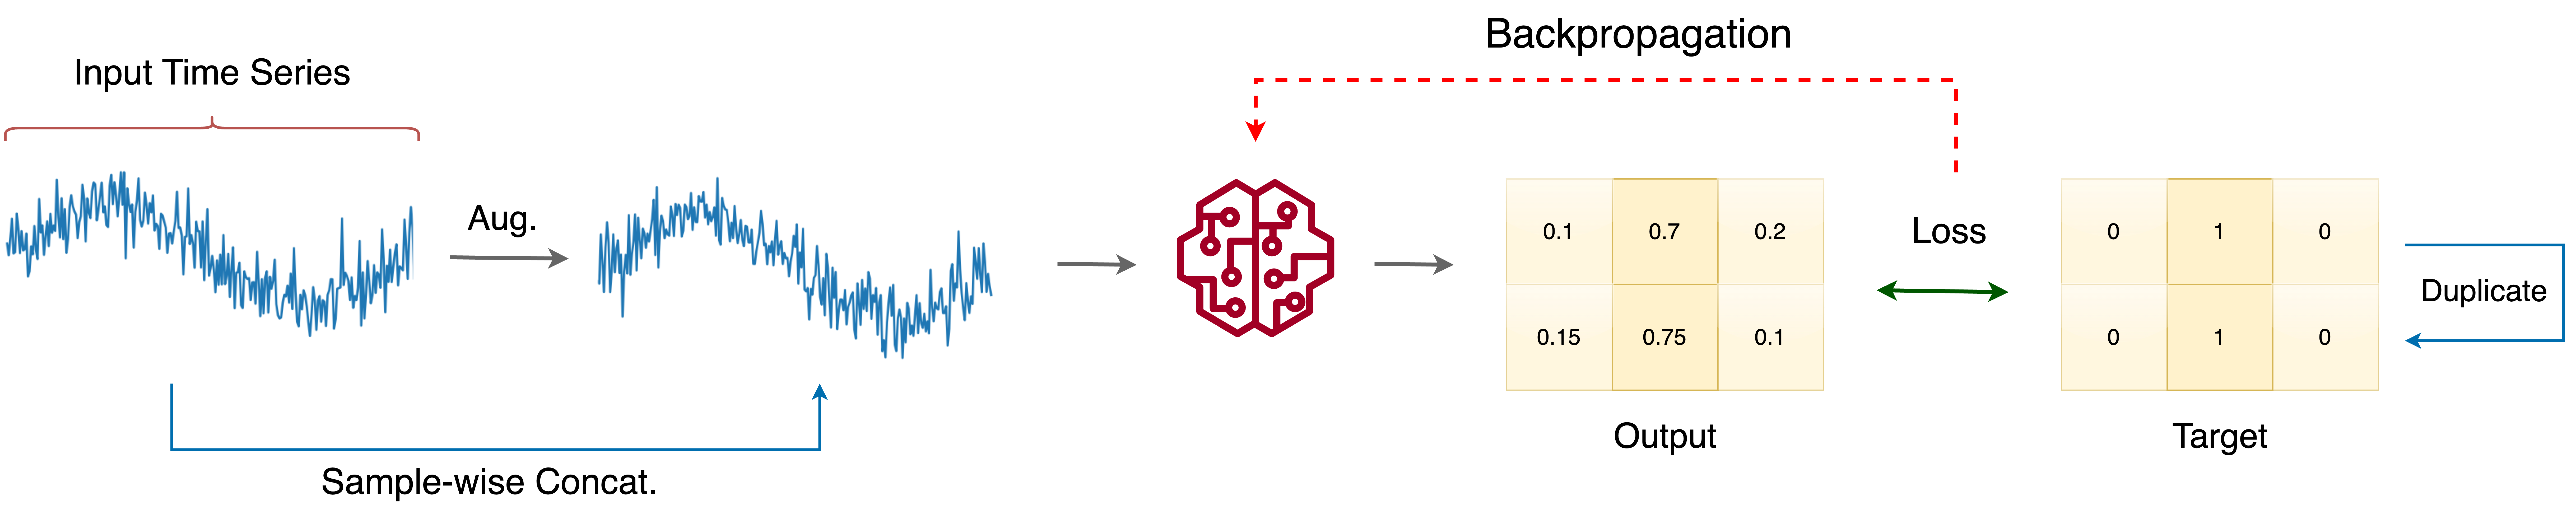
\includegraphics[width=1.0\textwidth, height=1.0\textheight, keepaspectratio]{./images/tsc_framework.drawio.png}

\caption{Training pipeline for time series classification using augmentation. An input sample is passed through an augmentation module to generate synthetic sequences, which are concatenated with the original input on a sample-wise basis—effectively doubling the sample size. Only the inputs are augmented; class labels remain unchanged and are duplicated to match the output. The model computes output probabilities, and the cross-entropy loss is backpropagated. Adapted from the paper~\cite{chen2023fraugfrequencydomainaugmentation}.}

    \label{fig:tsc_fw}
\end{figure}



Figure~\ref{fig:tsc_fw} demonstrates the training pipeline employing augmentation techniques for a single sample, adapted from~\cite{chen2023fraugfrequencydomainaugmentation}. Unlike time series forecasting, only input data $\mathbf{X}$ without class labels undergoes an augmentation process and is concatenated on a sample-wise basis, effectively doubling the sample size. Upon generating the probabilities, the loss (Eq.~\ref{eq: cross}) between the output predictions and the corresponding (duplicated) targets is computed and subsequently backpropagated to the model. Data augmentation techniques for time series classification improve accuracy, minimize loss, and strengthen model robustness and generalization.
 



\section{Approaches} \label{sec: approaches}

% Define all approaches here quickly and define challenges

Numerous augmentation methods have been proposed for time series forecasting, but designing an augmentation technique that maintains temporal dynamics and coherence remains challenging. Augmentation for time series forecasting requires significantly more careful design than augmentation for time series classification~\cite{zhang2023diversecoherentaugmentationtimeseries}. Popular transformation-based augmentations such as jittering, rotation, scaling~\cite{Um_2017}, permutation~\cite{Pan2020}, and window slicing~\cite{leguennec:halshs-01357973} have proven effective for time series classification. However, as described in Section~\ref{section:transformation}, these methods fail to perform well in forecasting tasks due to their disruptive effect on the temporal structure.

Frequency-based augmentations have gained significant popularity for time series forecasting. One of the early approaches, RobustTAD~\cite{gao2021robusttadrobusttimeseries}, applies perturbations to either the magnitude or phase of the frequency spectrum. Methods such as FreqAdd~\cite{freqadd} and FreqPool~\cite{freqpool} were designed following RobustTAD. In FreqAdd, a low-frequency component is selected, and its magnitude is set to half of the maximum magnitude in the corresponding channel, whereas FreqPool compresses the frequency spectrum to focus on dominant frequencies~\cite{freqadd, freqpool}.

Frequency Masking (FreqMask) and Frequency Mixing (FreqMix)~\cite{chen2023fraugfrequencydomainaugmentation} are two of the most widely adopted techniques in recent research. FreqMask involves masking specific components in the frequency domain, while FreqMix combines frequency components based on a defined hyperparameter \textit{rate}~\cite{chen2023fraugfrequencydomainaugmentation}. More recently, Wavelet Masking (WaveMask) and Wavelet Mixing (WaveMix)~\cite{arabi2024wavemaskmixexploringwaveletbasedaugmentations} have been introduced, demonstrating that augmentation can be further improved by using the discrete wavelet transform (DWT) instead of the fast Fourier transform (FFT). Unlike FFT, DWT captures both time and frequency domain characteristics by constructing overlapping time windows~\cite{arabi2024wavemaskmixexploringwaveletbasedaugmentations}. The latest research proposes an augmentation method called Dominant Shuffle~\cite{zhao2024dominantshufflesimplepowerful}, which claims to outperform all previously introduced methods. However, as discussed in Section~\ref{sec: problem}, Dominant Shuffle faces several challenges, including result inconsistency, out-of-distribution issues, and incorrect parameter configurations for model training, which undermine its reported advantages.

In the category of the decomposition-based augmentation methods, Spectral and Time Augmentation (STAug)~\cite{zhang2023diversecoherentaugmentationtimeseries} has shown better performance compared to approaches like weighted Dynamic Time Warping Barycentric Averaging (wDBA)~\cite{asd}, Moving Block Bootstrapping (MBB)~\cite{BERGMEIR2016303}, TimeGAN~\cite{timegan}, and others. STAug uses Empirical Mode Decomposition to decompose the time series and applies weighting in the time domain to generate augmented samples. wDBA and MBB are used for time series classification and forecasting but have failed to demonstrate success compared to frequency and decomposition-based methods for the forecasting tasks~\cite{zhang2023diversecoherentaugmentationtimeseries, chen2023fraugfrequencydomainaugmentation}. Another augmentation method, Upsample~\cite{upsample}, selects consecutive segments from a time series and linearly interpolates them to match the original length. All these augmentation methods for time series forecasting are discussed in detail in Section~\ref{sec: tsf_related}.


In contrast to time series forecasting, transformation-based augmentation methods have achieved success for time series classification tasks. Beyond the previously mentioned augmentation techniques, methods such as magnitude warping, time warping, and window warping have been explored, and window warping is ranked the third most important augmentation method (refer to Table~\ref{tab:augmentation_performance})~\cite{gao2024dataaugmentationtimeseriesclassification}.

Pattern-based augmentation methods, which incorporate transformation techniques to create patterns, have also emerged as some of the most effective strategies for classification tasks. Methods such as SuboPtimAl Warped time-series geNEratoR (SPAWNER)~\cite{s20010098}, wDBA~\cite{asd}, Random Guided Warping (RGW), and Discriminative Guided Warping (DGW)~\cite{iwana2020timeseriesdataaugmentation} rely on Dynamic Time Warping (DTW) or shapeDTW to calculate pair-wise distances. They differ mainly in their strategies for reference selection and use warping techniques to generate augmented samples. Currently, RGW, DGW, and their variants represent the state-of-the-art among augmentation methods for time series classification~\cite{gao2024dataaugmentationtimeseriesclassification}.

Finally, generative model-based and decomposition-based augmentations have been tested for classification tasks but have generally been found ineffective~\cite{gao2024dataaugmentationtimeseriesclassification, 10.1371/journal.pone.0254841}. Consequently, they have been excluded from our experimental protocols. For a detailed analysis of each augmentation method within classification contexts, refer to Section~\ref{sec: tsc_related}.


\section{Research Problem}
\label{sec: problem}

The latest developments in data augmentation for time series forecasting have been characterized by the introduction of innovative techniques, including the most recent Dominant Shuffle. The authors assert that they have overcome the drawbacks of previous augmentation techniques, such as FreqMask/FreqMix, FreqAdd, STAug, and others, commonly facing out-of-distribution challenges. Figure~\ref{fig:ood} depicts this challenge by showcasing t-distributed Stochastic Neighbor Embedding (t-SNE) visualizations of feature spaces derived from various augmentations. The authors assert that Dominant Shuffle diminishes external noise better than other augmentation methods and achieves superior outcomes relative to all current techniques. Additionally, they performed a comprehensive assessment across different model architectures, encompassing both long-term and short-term forecasting tasks, while comparing their augmentation method to the most recent augmentation techniques known to us~\cite{zhao2024dominantshufflesimplepowerful, freqadd, zhang2023diversecoherentaugmentationtimeseries, chen2023fraugfrequencydomainaugmentation}.

\begin{figure}[h!]
    \centering
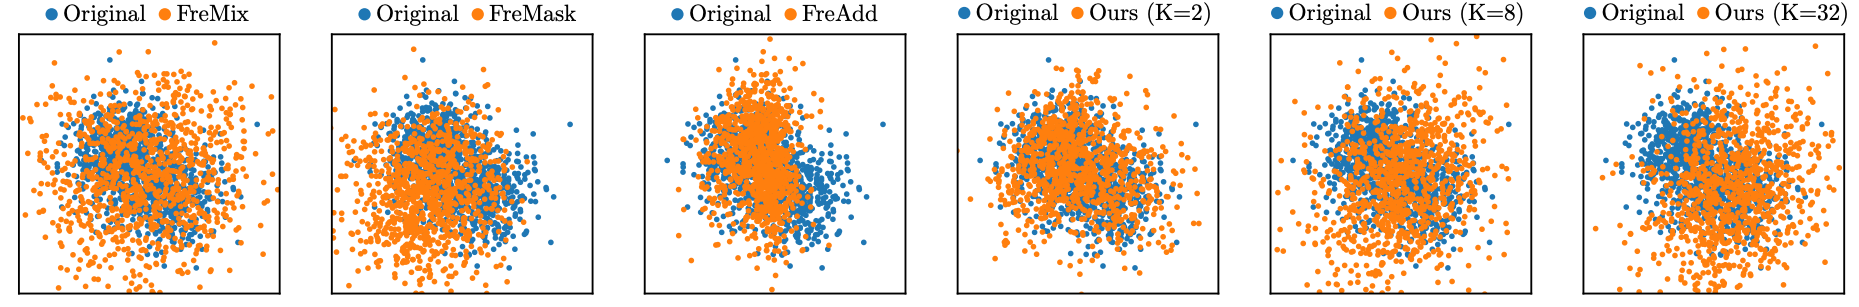
\includegraphics[page=1, width=1.0\textwidth]{./images/ood.png}
    \caption{t-SNE visualization of features of various augmentation methods~\cite{zhao2024dominantshufflesimplepowerful}.}
    \label{fig:ood}
\end{figure}

Despite these claims, several critical issues can be identified in their study. The first major issue is that the authors did not correctly reproduce the original models' hyperparameter settings, as the paper's reviewers reported. This misconfiguration led to a situation where, across many experiments, models trained with augmentations performed worse than their non-augmented counterparts. Additionally, the Dominant Shuffle technique often employed a high shuffling parameter (K), which, as visualized in Figure~\ref{fig:ood}, introduces external noise rather than mitigating it~\cite{zhao2024dominantshufflesimplepowerful}. The second primary concern is the inconsistency of results. When Dominant Shuffle was run multiple times (five different initializations), it frequently failed to achieve the superior performance claimed in the original paper, sometimes even underperforming compared to baseline methods, which is confirmed in our experimentations (see Chapter~\ref{chapter:experiments}). Finally, from a practical standpoint, Dominant Shuffle is computationally expensive relative to other methods like FreqMask/FreqMix and FreqAdd, a finding we confirm in the ablation study (see Table~\ref{tab:augmentation_comparison}) using the publicly available code. Given these observations, there remains a substantial need for a carefully designed augmentation method explicitly tailored for time series forecasting tasks.


The primary aim of this thesis is to design a novel patch-based augmentation method for time series data, drawing inspiration from the successes of similar approaches in the computer vision domain. The goal is not only to achieve superior predictive performance compared to existing time series augmentation methods but also to reduce the external noise introduced by augmentation and to mitigate the domain gap between augmented and original data.  Furthermore, another goal is to establish an augmentation framework applicable across diverse time series tasks, such as time series classification, requiring only minimal modification.

Another important contribution of this thesis is the establishment of a fair experimental protocol, ensuring that the evaluation metrics for models without augmentation match those reported in the original studies. In this way, this thesis provides not only a novel augmentation design but also a rigorous comparative study across both time series forecasting and time series classification domains.


\section{Research Questions}

This master's thesis aims to address the following research questions:

\begin{enumerate}
    \item  How does the proposed patch-based augmentation technique perform compared to existing augmentation methods across various time series forecasting and classification tasks?
    \item  Can the proposed augmentation method enhance model generalization and robustness without introducing significant external noise?
    \item  Can the proposed augmentation framework, with minimal adaptation, be effectively applied to both time series forecasting and classification tasks, providing a flexible solution for future research and applications?
    \item  Are all experimental setups and evaluation protocols implemented fairly to ensure a valid comparison between models with and without augmentation?
\end{enumerate}

These research questions form the foundation for the development, evaluation, and analysis presented throughout this thesis.


\section{Contributions}

The key contributions of this study include:

\begin{itemize}
    \item We propose a novel augmentation method, \textbf{Temporal Patch Shuffle (TPS)}, which consistently outperforms existing augmentation techniques  across seven benchmark datasets for long-term and four for short-term time series forecasting.

    \item TPS not only achieves state-of-the-art results but also improves generalization and robustness while introducing minimal noise, making it a reliable and efficient augmentation strategy.

    \item We extend \textbf{TPS} to the time series classification domain and introduce a new variant, \textbf{Temporal Index Patch Shuffle (TIPS)}, specifically designed for classification tasks. Both TPS and TIPS, individually and in combination, demonstrate superior performance compared to existing augmentation methods on both univariate and multivariate time series classification benchmarks.

    \item We conduct extensive ablation studies to analyze the behavior of our proposed method under various settings, examining their individual components, parameter sensitivity, and robustness to different sources of noise and distribution shifts.

    \item We address flaws in prior experimental protocols by ensuring fair and consistent evaluation, including the correct use of original model hyperparameters within a reasonable computational budget. Additionally, we replicate several augmentation methods from prior works that lacked publicly available code, ensuring reproducibility in the forecasting domain.

    \item Beyond proposing new methods, our master's thesis provides a comprehensive evaluation of existing augmentation techniques, benchmarking them under consistent conditions using recent models for both time series forecasting and classification. 
\end{itemize}
The codebase is available at \url{https://github.com/jafarbakhshaliyev/msc_thesis}.














% %%%%%%%%%%%%%%%%%%%%%%%%%%%%%%%%%%%%%%%%%

% %%%%%%%%%%%%%%%%%%%%%%%%%%%%%%%%%%%%%%%%%
 %!TEX root = ../Master_template.tex
\chapter{Related Work}



This chapter comprehensively summarizes the latest data augmentation methodologies designed for time series analysis. Time series tasks span a variety of domains; however, this work primarily focuses on two: \textbf{Time Series Forecasting (TSF)} and \textbf{Time Series Classification (TSC)}. Augmentation methods for forecasting are commonly categorized into four types: transformation-based, frequency-based, decomposition-based, and other approaches (refer to Section~\ref{sec: tsf_related}). For classification, augmentation methods are typically grouped into transformation-based, pattern-based, generative model-based, and decomposition-based categories (see Section~\ref{sec: tsc_related}).


Each category is discussed in detail, with formal definitions, mathematical formulations, pseudocode, and illustrative figures provided, where appropriate, to facilitate a deeper understanding of the augmentation methods. All mathematical representations in this chapter align with the formalism established in Section~\ref{section:formulation}.




\section{Time Series Forecasting } \label{sec: tsf_related}

\subsection{Transformation-based Augmentations} \label{section:transformation}


Transformation-based techniques include Gaussian noise injection~\cite{wen2019timeseriesanomalydetection}, window cropping~\cite{cui2016multiscaleconvolutionalneuralnetworks, Wen_2021}, window warping, and other methods~\cite{Wen_2021}. Initially developed in Computer Vision (CV), these methods have been adapted for time series analysis, specifically for tasks like time series classification and anomaly detection, showing significant effectiveness. These methods and more of them for the classification are detailed in Section~\ref{section:transformation2}. Nevertheless, the direct application of these augmentation techniques to TSF tasks generally does not produce significant advantages, as indicated by recent studies. The main factors contributing to the limited success in forecasting contexts are disturbances to the temporal order, such as introducing random noise or shifting the time series, or a lack of diversity in the generated augmented samples. These issues underscore the essential significance of preserving both diversity and coherence in augmentation methodologies tailored explicitly for forecasting tasks~\cite{Wen_2021, chen2023fraugfrequencydomainaugmentation, zhang2023diversecoherentaugmentationtimeseries, zhao2024dominantshufflesimplepowerful}. 



These traditional transformation-based augmentation methods were evaluated in the paper~\cite{chen2023fraugfrequencydomainaugmentation}, and the results indicate that they generally fail to improve performance over models trained without augmentation. Table~\ref{tab:Trad} reports the Mean Squared Error (MSE) for various models on the ETTh1 dataset with a prediction length of 96. As shown, most of these techniques—such as masking, flipping, and warping—tend to degrade performance and introduce distortions to the temporal structure. Other studies have similarly concluded that such transformations offer little to no benefit and distort the temporal dynamics of the time series signals, ultimately worsening model performance~\cite{Wen_2021, zhang2023diversecoherentaugmentationtimeseries, zhao2024dominantshufflesimplepowerful}.


\begin{table*}[h]
\centering

\begin{adjustbox}{max width=\textwidth}

\begin{tabular}{c|c|c|c|c|c|c|c}
\toprule
Method & Origin & Noise & Noise* & Mask-Rand. & Mask-Seg. &Flipping &Warping\\ \midrule
DLinear & 0.373 & 0.444 & \textbf{0.371} & 0.803 &0.448 & 0.544 &0.401  \\
FEDformer & \textbf{0.374} & 0.380 & 0.397 & 0.448 &0.433 & 0.420 &0.385  \\
Autoformer & \textbf{0.449} & 0.460 & 0.476& 0.608 & 0.568  & 0.446 &0.465  \\
Informer & 0.931 & 0.936 & 1.112 & \textbf{0.846} & 1.013 & 0.955 &1.265 \\\bottomrule
\end{tabular}
\end{adjustbox}
\vspace{-0.1cm}
\caption{MSE of various transformation-based data augmentation methods on the ETTh1 dataset with a prediction length of 96, as reported in~\cite{chen2023fraugfrequencydomainaugmentation}. “Origin” refers to training without augmentation. Across all four forecasting models, transformation-based augmentation methods tend to worsen performance.}
\label{tab:Trad}
\vspace{-0.3cm}
\end{table*}



\subsection{Frequency-based Augmentations}


Frequency-based methods, including time-frequency approaches, achieved significant popularity, resulting in the design and implementation of various techniques. These methods apply diverse augmentation strategies, including frequency masking, frequency mixing, perturbation of phase or magnitude of frequencies, shuffling of frequency components, and alteration of frequency components~\cite{chen2023fraugfrequencydomainaugmentation, zhao2024dominantshufflesimplepowerful, gao2021robusttadrobusttimeseries, freqpool, freqadd, arabi2024wavemaskmixexploringwaveletbasedaugmentations}. 


One of the foundational approaches in frequency-domain augmentation is RobustTAD~\cite{gao2021robusttadrobusttimeseries}, which applies perturbations to either the magnitude or phase of the frequency spectrum. Specifically, this method first obtains the frequency spectrum $F(\omega_k)$ of an input time series $x_t$ through the discrete Fourier transform (DFT):

\[ F(\omega_k) = \frac{1}{N}\sum_{t=0}^{N-1} x_t e^{-j2\pi kt/N}, \quad k=0,1,\dots,N-1,  \]


This spectrum can be decomposed into real and imaginary parts, represented as:

\[ F(\omega_k) = \Re[F(\omega_k)] + j\Im[F(\omega_k)], \]
where $\Re[F(\omega_k)]$ and $\Im[F(\omega_k)]$ are the real and imaginary parts of the spectrum respectively.

The amplitude spectrum $A(\omega_k)$ and phase spectrum $\theta(\omega_k)$  are derived as follows:

\[  A(\omega_k) = |F(\omega_k)| = \sqrt{\Re^2[F(\omega_k)] + \Im^2[F(\omega_k)]},  \]

and

\[ \theta(\omega_k) = \arctan\left(\frac{\Im[F(\omega_k)]}{\Re[F(\omega_k)]}\right) \]



To perform augmentation, RobustTAD selects segments of the frequency spectrum to modify. The length $K$ of each selected segment is determined proportionally by a hyperparameter ratio $r$: $K = r N'$ where $N'$ denotes the length of the spectrum~\cite{gao2021robusttadrobusttimeseries}.

For amplitude-based augmentation, the original amplitudes in the chosen segments are changed to values from a Gaussian distribution, which is controlled by a parameter for perturbation intensity. In the case of phase augmentation, the phase values within the selected segments are increased slightly by introducing controlled perturbations~\cite{gao2021robusttadrobusttimeseries}. While the original paper conducted experiments on anomaly detection, the studies~\cite{chen2023fraugfrequencydomainaugmentation, zhang2023diversecoherentaugmentationtimeseries, zhao2024dominantshufflesimplepowerful} have explored magnitude perturbation of RobustTAD for the multivariate TSF tasks. Phase perturbation has also been incorporated into RobustTAD for our experimentations.




Frequency Masking (FreqMask) and Frequency Mixing (FreqMix) are recent research studies on data augmentation for TSF that work on the frequency domain. They are straightforward but effective augmentation methods described in Figure~\ref{fig:freqmask}. FreqMask masks the signal's frequency components, eliminating specific events from the underlying system. On the other hand, FreqMix mixes frequencies from two randomly chosen series within the same batch, which exchange events between systems. To extract the frequency components for both methods, they rely on the fast Fourier transform (FFT)~\cite{chen2023fraugfrequencydomainaugmentation}. The complete pseudocode for these methods is available in Appendix~\ref{app:freqmask}.



\begin{figure}[h!]
    \centering
    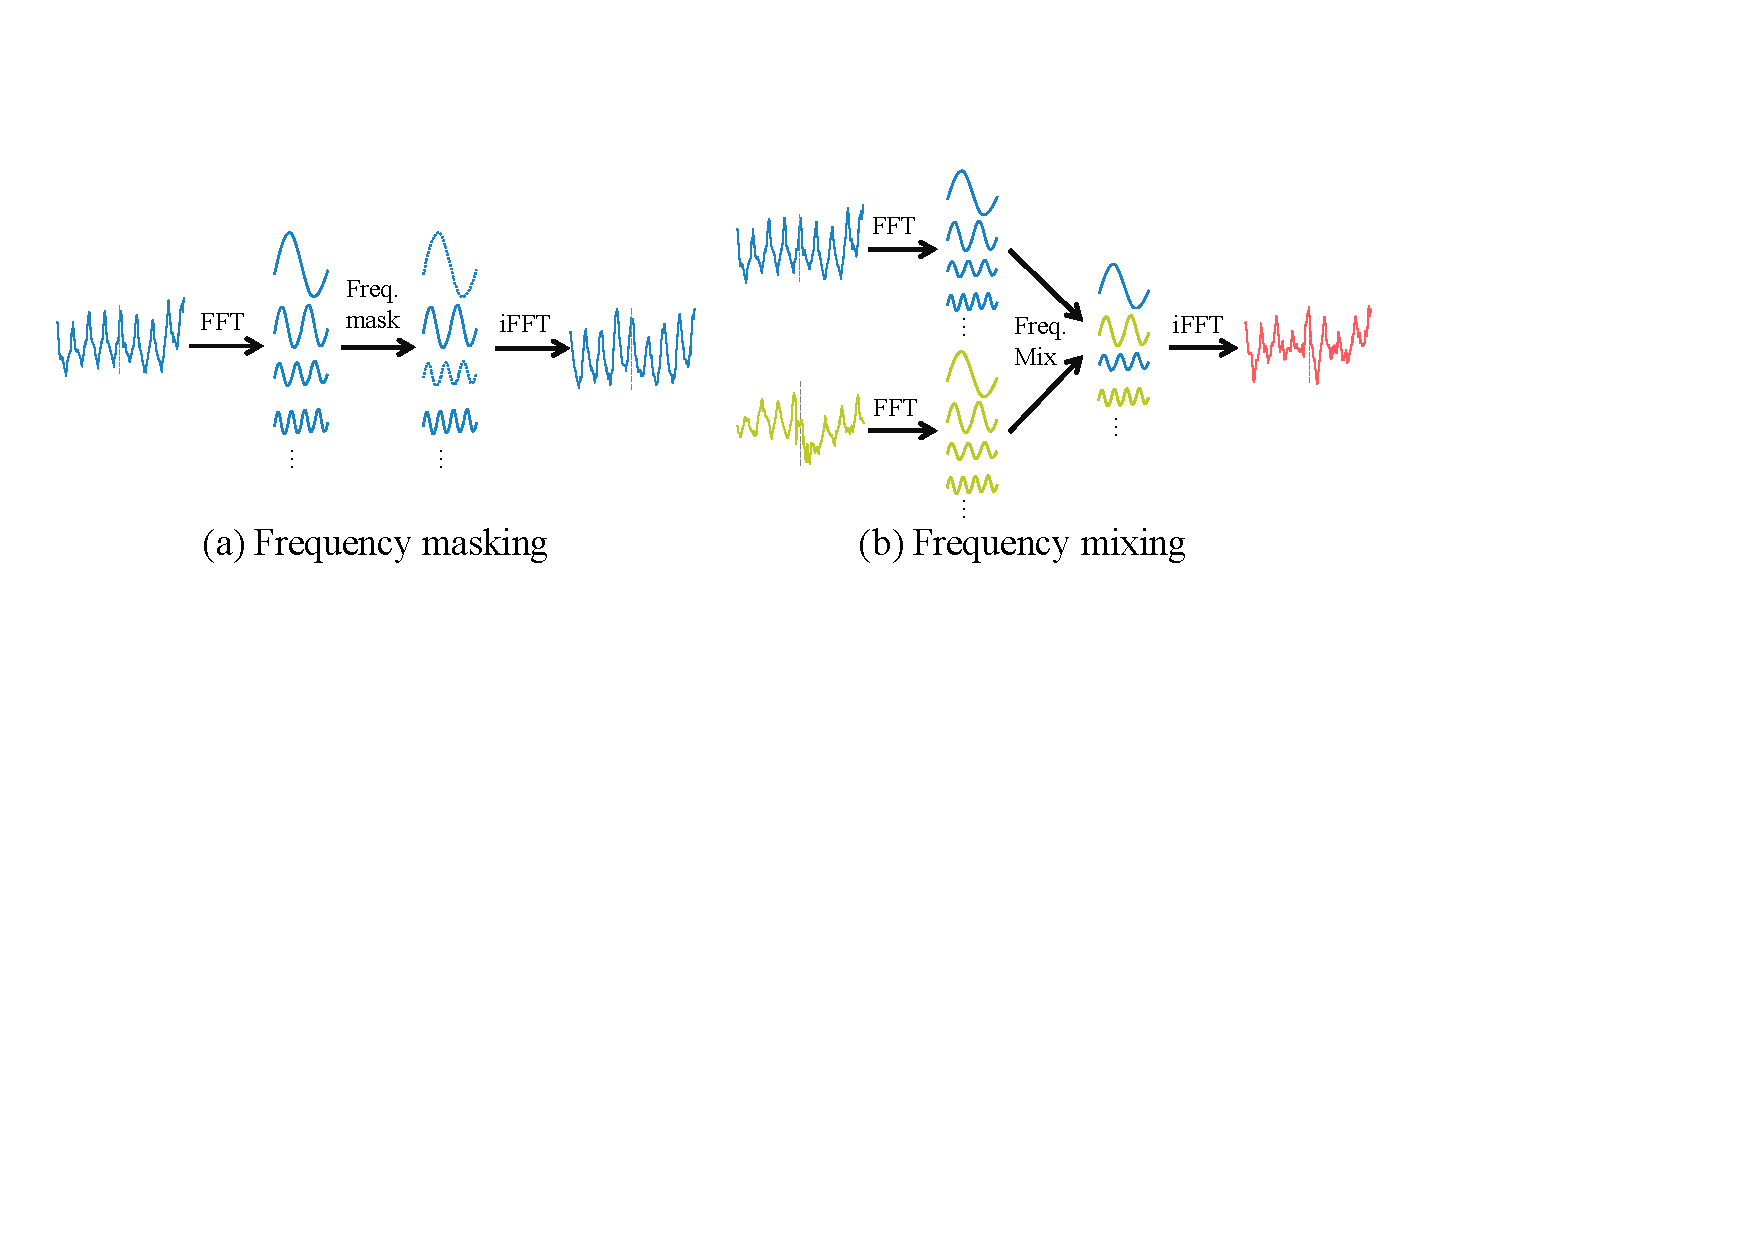
\includegraphics[page=1, width=0.9\textwidth]{./images/freqmaskmix.pdf}
\caption{Illustration of Frequency Masking and Frequency Mixing techniques. Both methods operate in the frequency domain by first applying a fast Fourier transform (FFT). Frequency Masking removes selected frequency components to suppress specific temporal patterns, while Frequency Mixing blends the frequency spectra of two series within the same batch to exchange dynamic characteristics~\cite{chen2023fraugfrequencydomainaugmentation}.}

    \label{fig:freqmask}
\end{figure}



% write about wavelet mask/mix add pictures only showing wavemask improvement. write description and the code.


Wavelet masking (WaveMask) and wavelet mixing (WaveMix) were introduced by~\cite{arabi2024wavemaskmixexploringwaveletbasedaugmentations} to address the limitations of FreqMask and FreqMix, which do not take the time domain into account. They are implemented the same way as FreqMask and FreqMix, but they apply the discrete wavelet transform (DWT) instead of the Fourier transform. Figure~\ref{fig:wavemask} illustrates the time-frequency analysis of the signal, and it shows the effectiveness of using wavelet transform to deliver frequency component information over time through different variable windows. WaveMask and WaveMix have been shown to outperform FreqMask and FreqMix methods on a small subset of datasets, indicating their potential for improved performance in TSF tasks~\cite{arabi2024wavemaskmixexploringwaveletbasedaugmentations}.






\begin{figure}[h!]
    \centering
    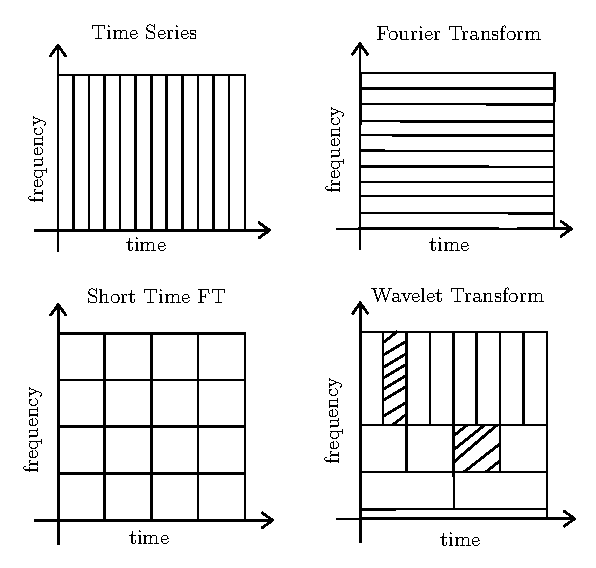
\includegraphics[page=1, width=0.6\textwidth]{./images/wavemask.pdf}
\caption{Time-frequency analysis methods, where the wavelet-based approach demonstrates how it captures localized frequency components using variable-sized windows~\cite{en16020764, arabi2024wavemaskmixexploringwaveletbasedaugmentations}.}
    \label{fig:wavemask}
\end{figure}


%write dominant shuffle and also say that they did not compare with WaveMask. add picture if there is peseduocode add it.




The paper by \cite{zhao2024dominantshufflesimplepowerful}  has mentioned that existing augmentations such as FreqMask and FreqMix may perturb the frequency components arbitrarily, which leads to significant deviations from the original time series data and introduce out-of-distribution (OOD) issues. The authors validate it through t-distributed stochastic neighbor embedding (t-SNE) visualizations. They have also proposed a new simple augmentation method named Dominant Shuffle and have conducted a comprehensive comparison with existing augmentation techniques. Dominant Shuffle obtains frequency components with the FFT and permutes randomly top $k$  dominant frequency components before reconstructing the augmented series. Figure~\ref{fig:domshuffle} depicts Dominant Shuffle augmentation, which changes the order of the three dominant frequency components. Their experimentations also include shuffling of not only dominant but also minor frequencies in the ablation study~\cite{zhao2024dominantshufflesimplepowerful}. 









\begin{figure}[h!]
    \centering
    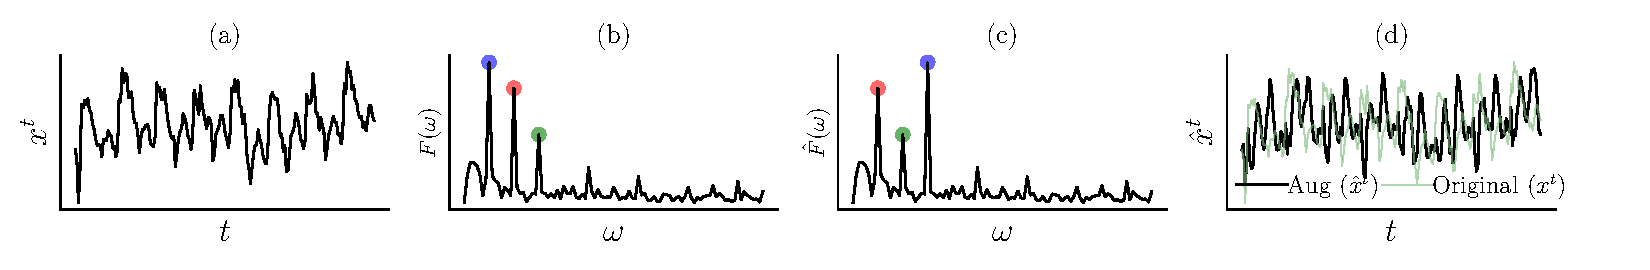
\includegraphics[page=1, width=0.9\textwidth]{./images/domshuffle.pdf}
    \caption{Illustration of the Dominant Shuffle augmentation technique, which permutes the top three dominant frequency components identified via FFT before reconstructing the time series~\cite{zhao2024dominantshufflesimplepowerful}.}
    \label{fig:domshuffle}
\end{figure}


%write freqadd, freqpool explain much possible you can. maybe two small paragprahs.

Other frequency-based augmentation techniques are FreqAdd~\cite{freqadd} and FreqPool~\cite{freqpool}, where the former modifies the frequency component and the latter compresses the frequency spectrum. FreqAdd chooses a low-frequency component after obtaining frequency components with FFT and sets its magnitude to half of the maximum magnitude in the corresponding channel. Experimental results demonstrate that FreqAdd reaches peak performance when it modifies a single, low-frequency component, whereas low-frequency components pertain to the lower-frequency spectrum segment and contain slower fluctuations. On the other hand, FreqPool compresses the frequency spectrum by applying max-pooling along the frequency axis, which diminishes spectral resolution yet retains dominant frequency information~\cite{freqadd, freqpool}. \cite{zhao2024dominantshufflesimplepowerful} conducted a comprehensive evaluation of these augmentation strategies, validating their effectiveness, especially in multivariate TSF contexts.



\subsection{Decomposition-based Augmentations} \label{section:decom}







Decomposition-based methods primarily apply techniques such as Seasonal and Trend decomposition using Loess (STL)~\cite{cleveland1990stl} or Empirical Mode Decomposition (EMD)~\cite{huang1998empirical}. Early approaches applies EMD to decompose time series into Intrinsic Mode Functions (IMFs), which represent frequency components ranging from high-frequency oscillations to low-frequency variations. The residual is incorporated with each occurrence of an IMF, serving as a data augmentation method that filters out high-frequency noise~\cite{nam2020data}. Nonetheless, the drawback of this technique is that it fails to incorporate the time domain~\cite{zhang2023diversecoherentaugmentationtimeseries}. 

The recent augmentation method, Spectral and Time Augmentation (STAug), proposed by \cite{zhang2023diversecoherentaugmentationtimeseries}, relies on frequency and time domains. Figure~\ref{fig:staug} illustrates the methodology of STAug. It selects two time-series sequences randomly and decomposes both into multiple IMFs by utilizing EMD. After assigning weights from a uniform distribution for these decomposed components, they are recombined in a time-domain signal through a Mixup strategy~\cite{zhang2018mixupempiricalriskminimization} with a parameter $\lambda$ sampled from a Beta distribution. This step adds diversity by combining elements from various sequences in the time domain, using both temporal coherence and spectral attributes. The experimental results of the paper validated that STAug outperforms existing augmentation techniques across various benchmark datasets, including RobustTAD and TimeGAN~\cite{zhang2023diversecoherentaugmentationtimeseries}.




\begin{figure}[h!]
    \centering
    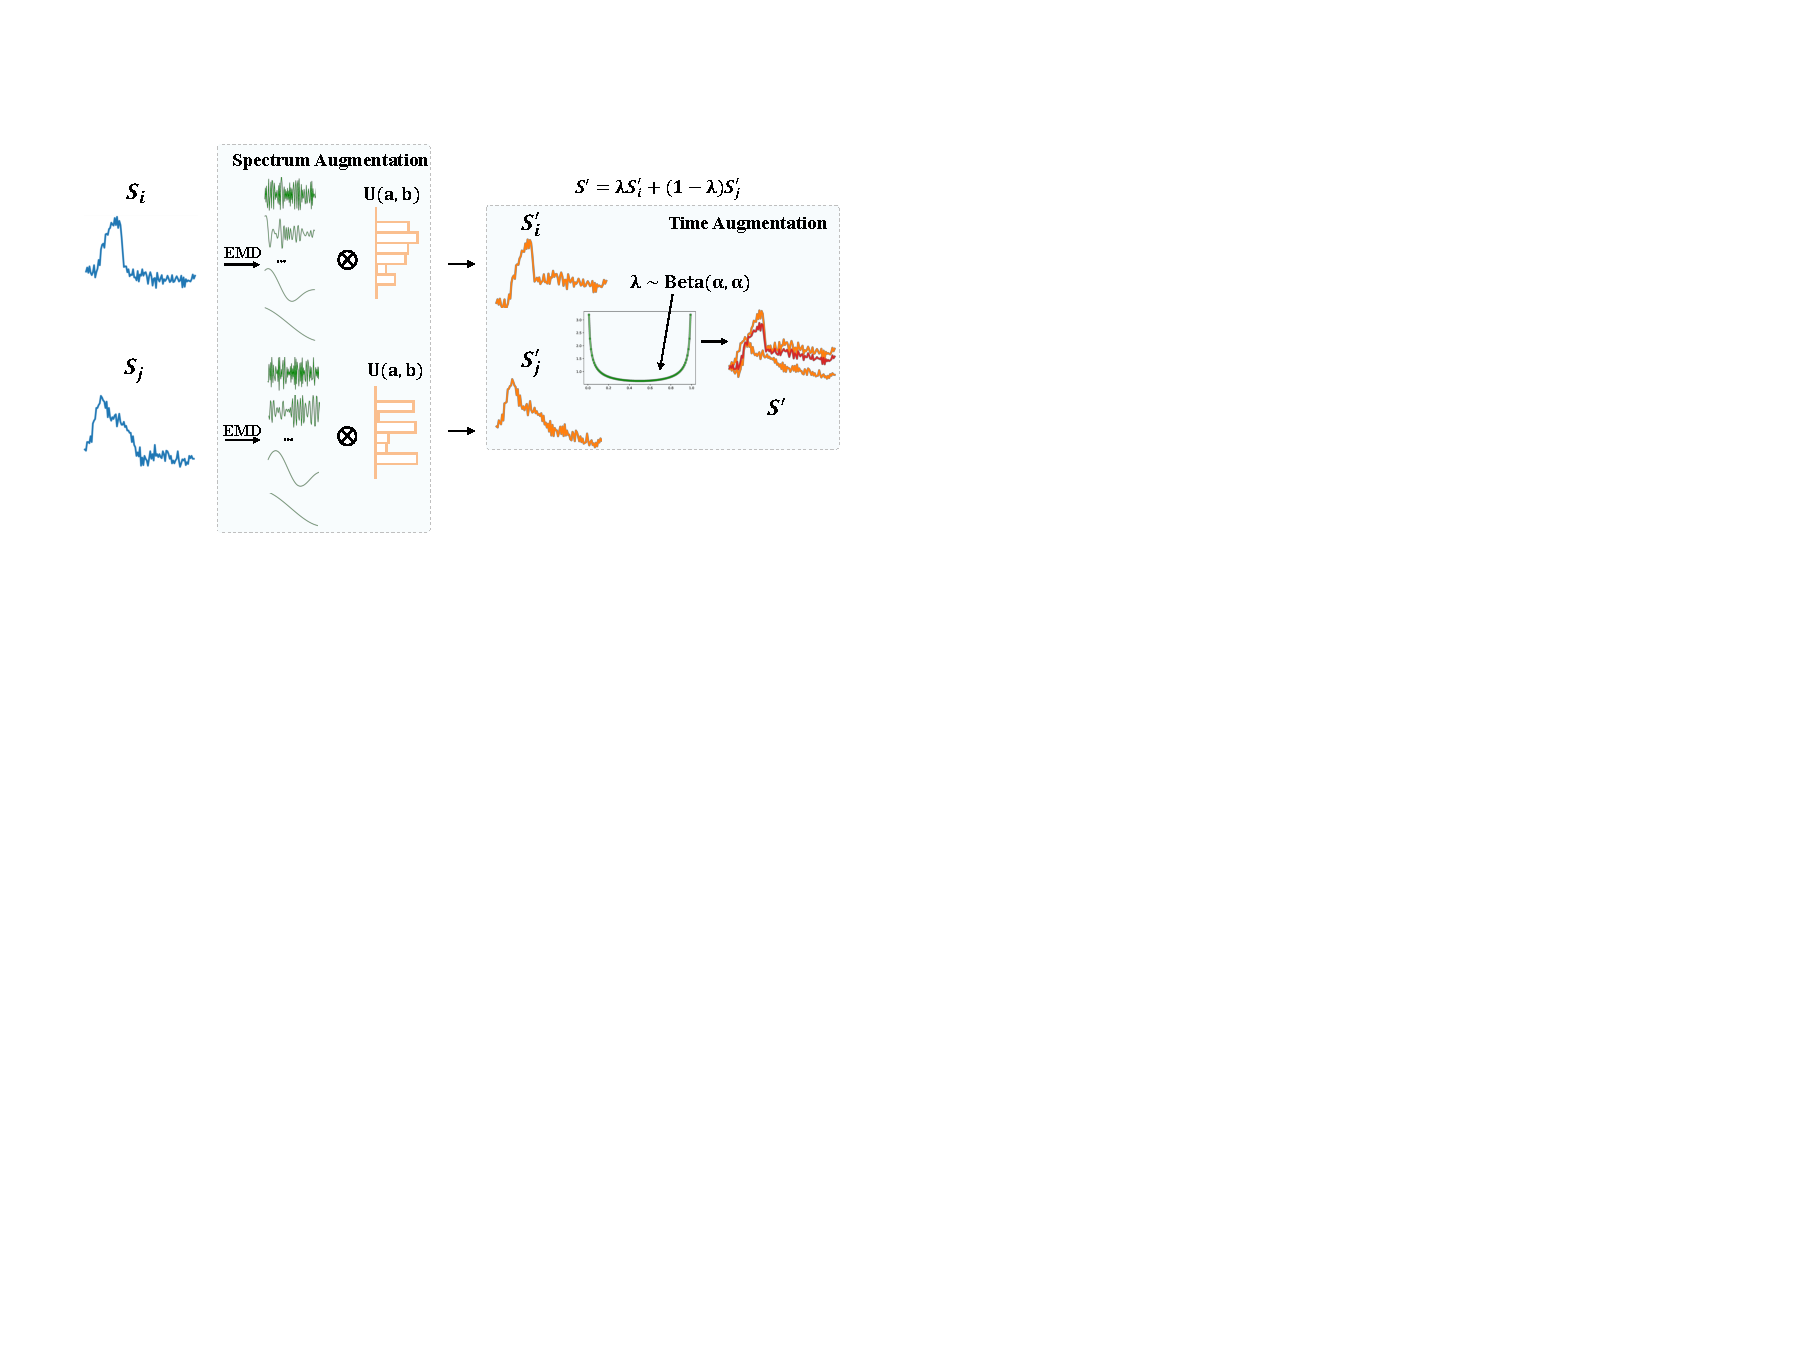
\includegraphics[page=1, width=0.9\textwidth]{./images/staug.pdf}
    \caption{STAug: A decomposition-based augmentation method that applies Empirical Mode Decomposition (EMD) and recombines IMFs using a Mixup strategy in the time domain~\cite{zhang2023diversecoherentaugmentationtimeseries}.}
    \label{fig:staug}
\end{figure}



\subsection{Other Approaches} \label{section:other}

This section presents various augmentation techniques grouped under \emph{other approaches}, including Moving Block Bootstrapping~\cite{mbb}, weighted Dynamic Time Warping Barycentric Averaging~\cite{asd}, Upsampling~\cite{upsample}, and generative model-based augmentations (e.g., TimeGAN~\cite{timegan}). These methods are categorized separately because they do not decompose time series nor explicitly function within frequency domains, amplitude spectra, or wavelet domains, in contrast to the previously reviewed techniques~\cite{asd, mbb, upsample, timegan}. 

The Upsample augmentation technique selects consecutive segments from the original time series, and a hyperparameter ratio $r$ determines the length of this segment. This segment is expanded to the original length of time series $T$ through linear interpolation, which helps to highlight data areas that forecasting models may overlook. As expressed by the authors, this technique operates as a ”magnifying glass”, enabling forecasting models to focus on local structures and intricate temporal patterns. The Upsample method has been evaluated against various augmentation methods, including fundamental and advanced techniques, primarily within univariate forecasting tasks. Empirical evidence shows that Upsample consistently surpasses alternative methods in predictive accuracy~\cite{upsample}. The method is assessed in multivariate forecasting contexts, where it exhibited successful results in the paper~\cite{zhao2024dominantshufflesimplepowerful}. Considering these documented results, the Upsample technique is incorporated into the empirical evaluations performed in this thesis study. 




% ASD

Different augmentation techniques using Dynamic Time Warping (DTW) to calculate pair-wise distances of training samples exist, and one of them is Dynamic Time Warping Barycentric Averaging (DBA), which generates augmented samples by averaging time series sets. There is another version called weighted DBA (wDBA), which assigns weights through the contribution of each time series toward the final one. \cite{asd} have proposed three versions of these augmentations based on the weighting: Average All (AA), Average Selected (AS), and Average Selected with Distance (ASD). wDBA with ASD is considered augmentation in our experimentation protocol and evaluated against other augmentation methods in earlier and recent papers for TSF. Specifically, after calculating the distances with DTW, wDBA applies an exponentially weighted sum to each sample’s top 5 closest neighbors to generate an augmented sample. This method is computationally expensive compared to the other methods in the experimentation. In the literature, this method is referred to interchangeably as ASD or wDBA; in this thesis, we consistently refer to it as wDBA~\cite{asd, mbb, chen2023fraugfrequencydomainaugmentation, zhang2023diversecoherentaugmentationtimeseries, zhao2024dominantshufflesimplepowerful}.





% MBB



Moving Block Bootstrapping (MBB) is used as an augmentation technique for forecasting tasks and is evaluated against wDBA. It first decomposes the signal into trend, seasonal, and remainder through STL~\cite{cleveland1990stl}. It perturbs the remainders with bootstrapping and then adds seasonal and trend components to create a new bootstrapped time series~\cite{mbb, BERGMEIR2016303}. For STL, the implementation from the Python package \textit{statsmodels} is used, and for bootstrapping on the remainder part, \textit{MovingBlockBootstrap} from the Python package \textit{arch} is used. This method is computationally expensive compared to the other augmentations, but it has been evaluated against all methods in recent papers~\cite{chen2023fraugfrequencydomainaugmentation, zhao2024dominantshufflesimplepowerful, zhang2023diversecoherentaugmentationtimeseries}. The MBB augmentation technique has also been added to our experimentation protocols.

% generative model-based augmentation (GAN)

Augmentations based on generative models, such as TimeGAN, are omitted from our augmentation protocol for forecasting and classification tasks. The exclusion from the forecasting task is because these methods are computationally intensive, as they rely on external training, unlike the mentioned techniques. Additionally, STAug surpasses TimeGAN, as documented in the paper~\cite{zhang2023diversecoherentaugmentationtimeseries}, and STAug is incorporated in our evaluation. The paper~\cite{chen2023fraugfrequencydomainaugmentation} highlighted that dataset augmentation methods based on synthetic generation, such as TimeGAN, introduce unexpected noise. All of these provide justifications for its exclusion from our evaluations. For generative model-based methods and reasons for exclusion from classification settings, refer to Section~\ref{section:gan}.






\section{Time Series Classification} \label{sec: tsc_related}

\subsection{Transformation-based Augmentations} \label{section:transformation2}


Several transformation-based augmentations are concisely outlined in Section~\ref{section:transformation}; these methodologies are typically derived from techniques initially developed in CV. Jittering~\cite{Um_2017} is a magnitude-based transformation that perturbs each time step of the signal by incorporating Gaussian noise. The augmented sequence $\mathbf{S}$ is formally defined as:

\[ \mathbf{S} = \mathbf{X} + \mathbf{G} \]

where $\mathbf{G} \in \mathbb{R}^{T \times C}$ and each element $g_{i,j} \sim \mathcal{N}(\mu, \sigma^2)$ is independently sampled from a Gaussian distribution characterized by mean $\mu$ and variance $\sigma^2$~\cite{10.1371/journal.pone.0315343, 10.1371/journal.pone.0254841}.

Rotation~\cite{10.1371/journal.pone.0254841} is a magnitude transformation method utilized for multivariate time series analysis. It transforms the input by adjusting the alignment of its values across channels. The transformed series $\mathbf{S}$ is derived as follows:

\[ \mathbf{S} = \mathbf{X} \cdot \mathbf{R} \]

where $\mathbf{R} \in \mathbb{R}^{C \times C}$ denotes a random rotation matrix, commonly produced using orthonormal basis vectors or parameterized by angles $\theta$. Alternatively, a straightforward variant involves using random sign alterations and channel rearrangements:

\[ \mathbf{S}{:, j} = \epsilon_j \cdot \mathbf{X}{:, \pi(j)}, \]

where $\epsilon_j \in \{-1, 1\}$ and $\pi$ denotes a random permutation of channel indices~\cite{10.1371/journal.pone.0315343}.

Scaling~\cite{Um_2017} is a magnitude-based transformation that alters the amplitude of a time series by applying a random scaling factor. The augmented sequence $\mathbf{S}$ is defined as:

\[ \mathbf{S} = \alpha \cdot \mathbf{X},  \]

where $\alpha \in \mathbb{R}$ is a scalar drawn from a normal distribution centered around one~\cite{10.1371/journal.pone.0254841}.





Magnitude Warping (MW)~\cite{10.1371/journal.pone.0254841} implements smooth, non-uniform modifications in the amplitude of a time series through applying a time-dependent scaling function. Rather than using a fixed multiplier, MW modulates at each time step with a smoothly varying curve, allowing the signal to display localized fluctuations in magnitude over time. The augmented version $\mathbf{S}$ is formally defined as:

\[ \mathbf{S}_{i,:} = \alpha_i \cdot \mathbf{X}_{i,:}, \quad \text{for } i = 1, \dots, T, \]

where $\alpha = (\alpha_1, \dots, \alpha_T) \in \mathbb{R}^T$ denotes a continuous scaling sequence produced by applying a cubic spline function $CS(u)$ to knots $u=(u_1, \dots, u_I) \in \mathbb{R}^I$. The spline is formed by using a limited number of control points (knots), each drawn from a distribution $\mathcal{N}(1, \sigma^2)$ to incorporate random but smooth variations. The number of knots $I$ and the standard deviation $\sigma$ are the hyperparameters for this augmentation method~\cite{10.1371/journal.pone.0315343}.


Window Slicing (WS)~\cite{leguennec:halshs-01357973} is a time-domain augmentation method that extracts a contiguous subsegment from the original time series, thereby shortening its temporal length while maintaining its structural characteristics ($\mathbf{X}_{1:\tau, :}$ where $\tau$ is a hyperparameter such that $\tau < T$). The augmented sequence $\mathbf{S}$ is derived through linearly interpolating the segments to the original length $T$~\cite{10.1371/journal.pone.0315343}. 


Permutation and Random Permutation~\cite{Um_2017, Pan2020} are time-domain augmentation methods that reorganize the sequence of time slices: these methods partition the input sequence into segments and subsequently permute them using either fixed-length segments (Permutation) or variable-length segments (Random Permutation). The augmented series $\mathbf{S}$ is formally defined as:

\[ \mathbf{S} = (x_{\pi(1)}, x_{\pi(2)}, \ldots, x_{\pi(T)}), \]

where $\pi$ denotes a permutation of the time indices $\{1, 2, \dots, T\}$, generated through segment-wise shuffling~\cite{10.1371/journal.pone.0254841, 10.1371/journal.pone.0315343}.


Time Warping (TW)~\cite{Um_2017, Park_2019} is a time-domain  augmentation method that modifies the temporal part of a time series through nonlinear alteration of the time steps' progression. The augmented sequence $\mathbf{S}$ is formally defined as:


\[ \mathbf{S} = (x_{\tau(1)}, x_{\tau(2)}, \ldots, x_{\tau(T)}), \]

where $\tau(\cdot)$ is a time-warping function that transforms original time steps to new, smoothly modified positions. The function is formulated by interpolating a smooth curve, a cubic spline $CS(u)$, established over a series of knots $u$. The knot values are drawn from a normal distribution $\mathcal{N}(1, \sigma^2)$ to generate localized expansions and contractions in the temporal dimension. The resultant distorted index positions are subsequently used to extract samples from the original sequence, yielding a time-warped rendering of the input signal~\cite{10.1371/journal.pone.0254841}.


Window Warping (WW)~\cite{leguennec:halshs-01357973} is a localized variant of time-domain augmentation derived from TW. WW randomly selects a window from the original time series. Subsequently, it is either temporally stretched by a constant factor of $2$ or contracted by a factor of $0.5$. The scales $[0.5, 2]$ are adjustable based on the data. After these operations, the augmented sequence is resampled to retain the original temporal length $T$~\cite{10.1371/journal.pone.0315343}.


\subsection{Pattern-based Augmentations}

Pattern-based methods produce new augmented samples by extracting and recombining patterns inherent in the signal, in contrast to transformation-based methods, which modify the original time series with different transformations. SuboPtimAl Warped time series geNEratoR (SPAWNER)~\cite{s20010098} is a pattern-based method that generates patterns with suboptimal time warping. Suboptimal time warping forces a warping path through a random point by restricting the warping ability of DTW, which is described in Section~\ref{section:other}. Using it, SPAWNER averages two intra-class randomly chosen patterns by hyperparameter percentage $\tau$ of the time series length $T$ with a warping path boundary constraint. It also adds noise sampled from Gaussian distribution to further transform data and $\tau$ is set to 10\% in the experiments~\cite{10.1371/journal.pone.0254841}.


wDBA~\cite{asd} is another pattern-based method outlined in Section~\ref{section:other} for TSF. As mentioned, three weighting strategies are used: AA, AS, and ASD. AA assigns weights to all of the time series in a class by a flat Dirichlet distribution. In contrast, AS chooses a reference time series and assigns weights to two of the five nearest neighbors by a significant amount and the rest by a small amount. ASD is analogous to AS, except it assigns weights based on the distance to the reference and uses an exponentially weighted sum of the top five neighbors. ASD weighting strategy is utilized as it outperformed other weighting strategies in the context of TSC~\cite{asd, 10.1371/journal.pone.0254841}.



% RGW 

Random Guided Warping (RGW)~\cite{Um_2017} is a pattern-based augmentation that utilizes guided warping, which integrates time warping with pattern mixing methods. Guided warping adjusts the features of a sample to correspond with the time-step relations of a chosen reference. DTW aligns the features of these two time series. RGW generates augmentation sets from time-warped original time series utilizing the guidance of other intra-class patterns. This explains the integration of time warping with the pattern mixing method, which maintains the characteristics of one time series while aligning it with the pace of a random reference time series set. The benefit of using warping with a reference is that both local features and temporal intervals are present in the original time series data. The authors proposed  a different version of RGW that uses shapeDTW~\cite{ZHAO2018171} to improve DTW by achieving a finer alignment utilizing higher-level shape descriptors. The first step is to get subsequences from the time series using a stride of one and a length of W for each temporal point. The identity function is a straightforward mapping function from these segments to shape descriptors, so these subsequences act as local shape descriptors. Figure~\ref{fig:rgw} illustrates both of these augmentations~\cite{10.1371/journal.pone.0254841, iwana2020timeseriesdataaugmentation, ZHAO2018171}. In our experimentation protocol, we use RGW for the DTW version and RGWs for the shapeDTW one.




\begin{figure}[h!]
    \centering
    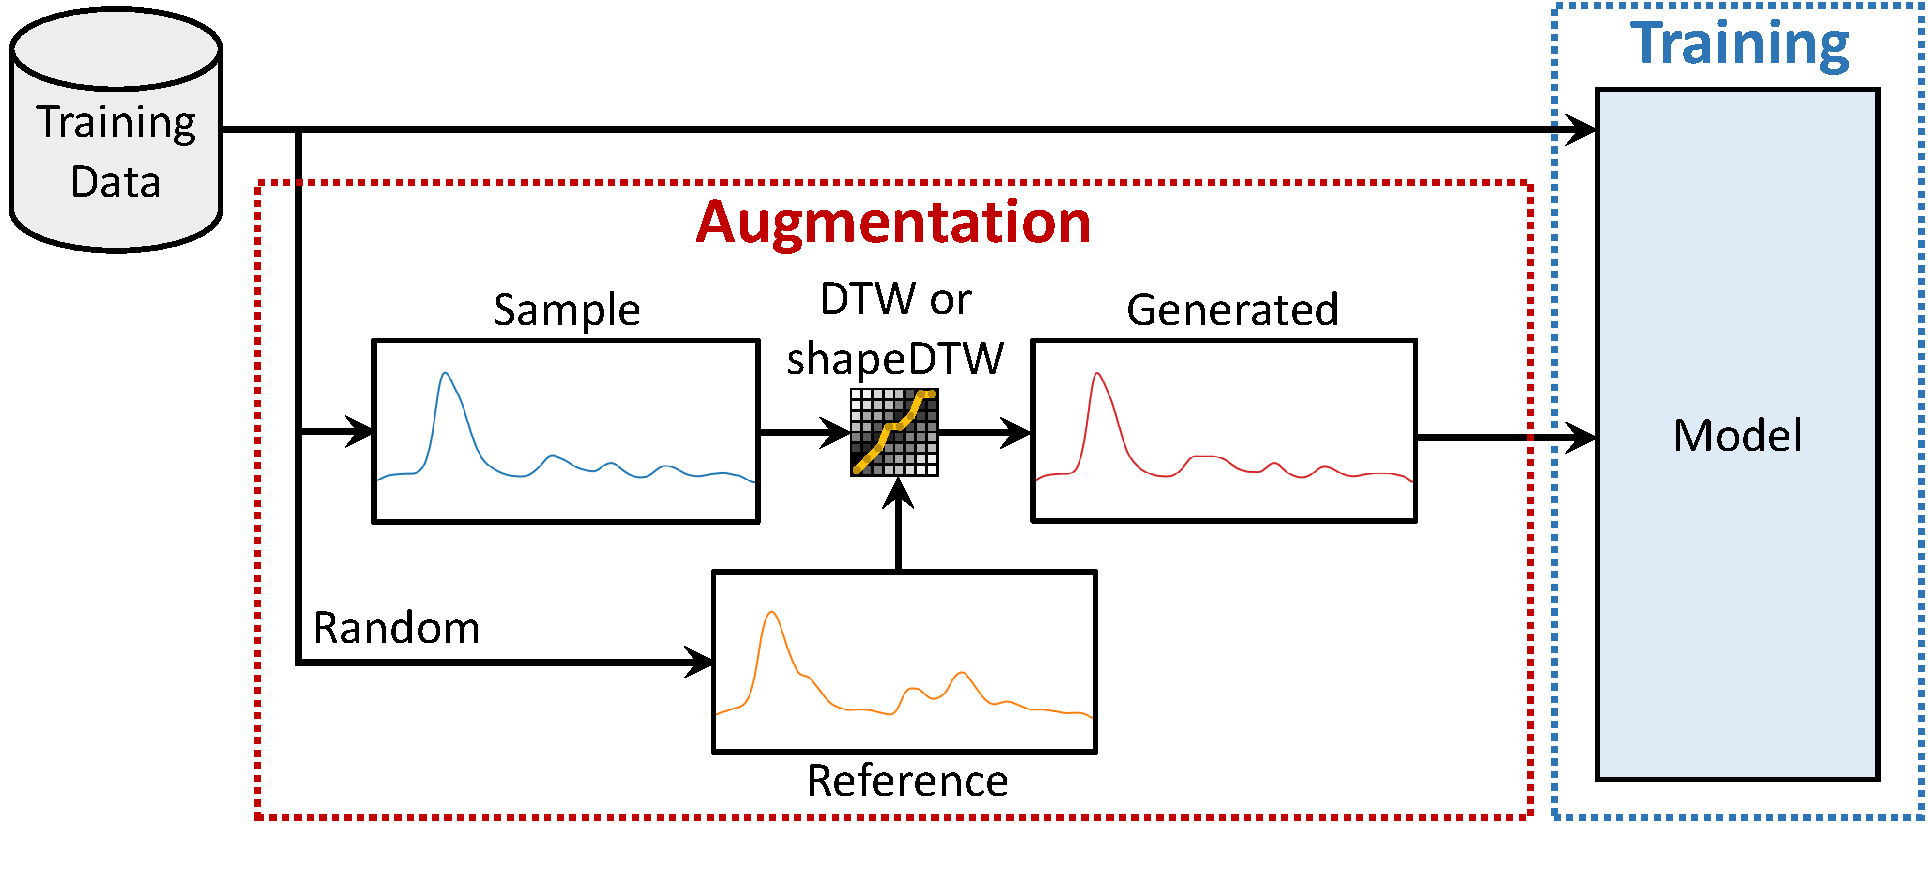
\includegraphics[page=1, width=0.9\textwidth]{./images/diagram_random.pdf}
\caption{Illustration of Random Guided Warping (RGW) and its variant using shapeDTW (RGWs)~\cite{iwana2020timeseriesdataaugmentation}. RGW aligns a time series with intra-class references using dynamic time warping (DTW), while RGWs leverages shapeDTW for enhanced alignment based on local shape descriptors~\cite{ZHAO2018171}.}
    \label{fig:rgw}
\end{figure}


Discriminative Guided Warping (DGW)~\cite{iwana2020timeseriesdataaugmentation} is similar to RGW, with the distinction that it uses multiple random (bootstrapped) subsets and directs from them for reference. The nearest centroid classifier utilizing DTW (or shapeDTW) distance determines the most discriminative directed reference from the bootstrapped sets. Rather than utilizing predictions from this classifier, a reference point with the largest distance between positive and negative centroids is selected. Utilizing this discriminatively selected reference, the temporal sequences are wrapped using  DTW or shapeDTW as previously described. Figure~\ref{fig:dgw} illustrates these techniques~\cite{iwana2020timeseriesdataaugmentation, 10.1371/journal.pone.0254841, ZHAO2018171}. In our experimental protocol, we utilize DGW for the DTW variant and DGWs for the shapeDTW variant.


\begin{figure}[h!]
    \centering
    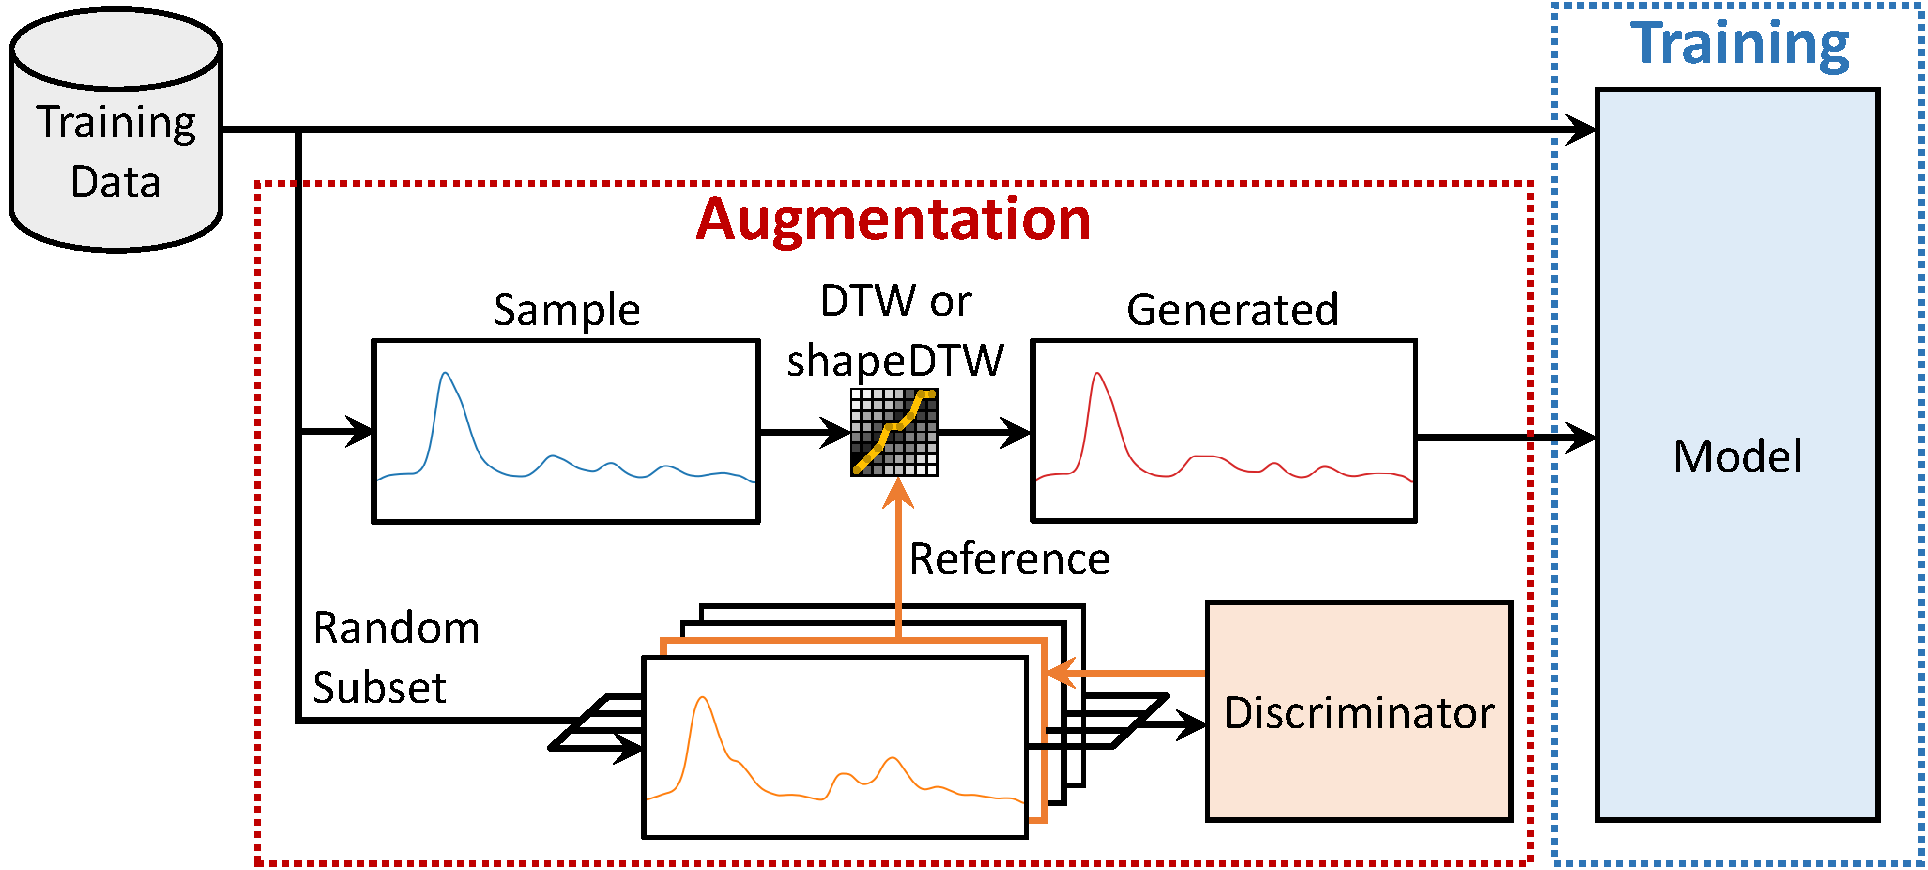
\includegraphics[page=1, width=0.9\textwidth]{./images/diagram_disc.pdf}
\caption{Illustration of the Discriminative Guided Warping (DGW) augmentation method~\cite{iwana2020timeseriesdataaugmentation}. DGW extends RGW by selecting a discriminative reference from bootstrapped intra-class subsets. The reference is chosen based on the largest centroid distance between classes using DTW or shapeDTW~\cite{ZHAO2018171}.}
    \label{fig:dgw}
\end{figure}




% new surveydi ela
\subsection{Generative Model-based Augmentations} \label{section:gan}



Deep generative models have become prominent in multiple fields, particularly image generation, due to their ability to produce realistic synthetic samples. Generative Adversarial Networks (GANs) are well-known among generative models for effectively generating diverse, realistic data that substantially improves training datasets. \cite{8512396} proposed a deep LSTM-based GAN for augmenting ECG and EEG signals. Subsequently, \cite{ramponi2019tcganconditionalgenerativeadversarial} introduced Temporal Convolutional GANs (TCGAN), which use one-dimensional convolutional layers to generate time series data. Conditional GANs (cGANs)~\cite{mirza2014conditionalgenerativeadversarialnets} have been utilized for data augmentation; however, \cite{9003933} compared a traditional GAN with a cGAN in the context of speech recognition and concluded that the traditional GAN exhibited better results on average~\cite{10.1371/journal.pone.0254841}. A recent generative model, TimeGAN, developed by \cite{timegan}, also expands these concepts to sequential data. Unlike traditional GANs, TimeGAN explicitly incorporates temporal dynamics, enabling the generation of highly realistic synthetic time series data~\cite{timegan}.



Figure~\ref{fig:timegan} outlines the architectural framework of TimeGAN, consisting of four primary components: an embedding function, a recovery function, a sequence generator, and a sequence discriminator. The embedding function transforms real sequences into a compacted latent space, while the recovery function reconstructs sequences from the latent representations. The generator creates latent representations of sequences, whereas the discriminator distinguishes between the latent embeddings of real and synthetic sequences. Unlike traditional GANs, TimeGAN optimizes unsupervised adversarial losses and supervised reconstruction losses, ensuring that the generated data is realistic and accurately represents the temporal dynamics of the original data~\cite{timegan}. 

\begin{figure}[h!]
    \centering
    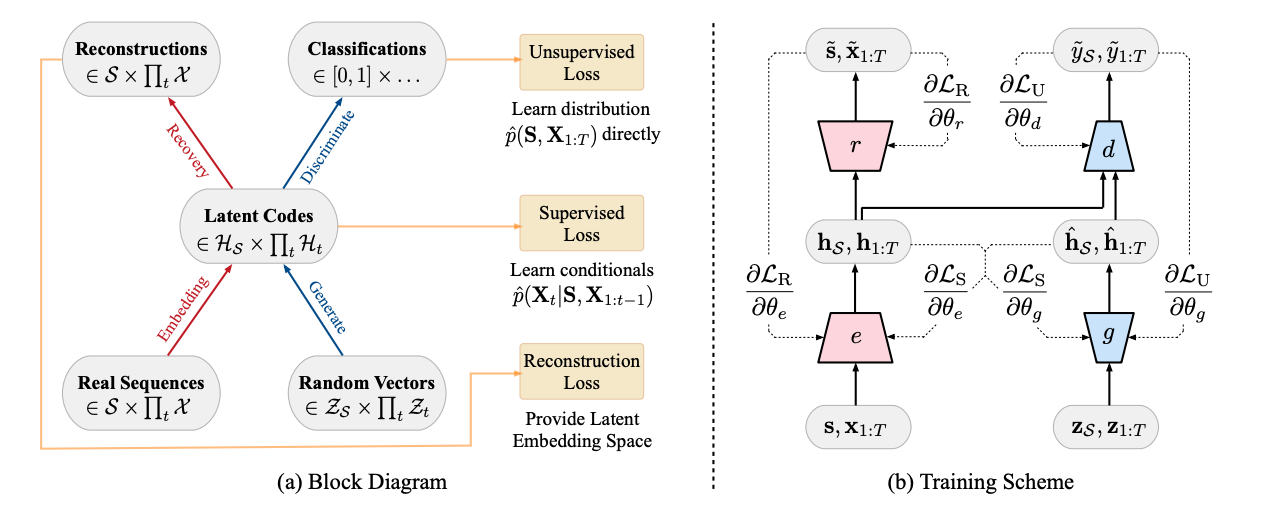
\includegraphics[page=1, width=0.9\textwidth]{./images/timegan.png}
\caption{TimeGAN architecture, consisting of an embedding function, recovery function, generator, and discriminator. The embedding-recovery pair maps time series to and from a latent space, while the generator and discriminator operate in this space to synthesize and evaluate sequences. TimeGAN combines adversarial and supervised losses to generate realistic time series that preserve temporal dynamics~\cite{timegan}.}

    \label{fig:timegan}
\end{figure}


In Section~\ref{section:other}, we mentioned that TimeGAN is removed from the experimentation protocol as it is computationally expensive, and other methods achieve better results for TSF. It is also true for TSC as the study~\cite{10.1371/journal.pone.0254841} has excluded it from the experimentations due to additional expensive external training. Other studies, such as \cite{gao2024dataaugmentationtimeseriesclassification} have shown that the GAN methods failed to generate realistic data (refer to Appendix~\ref{app:tscranking}), marking it the least effective augmentation, and \cite{10.1371/journal.pone.0315343} have indicated a marginal improvement over the baseline (see Table~\ref{tab:augmentation_performance}). These findings validated our decision to exclude them from our evaluations.







\subsection{Decomposition-based Augmentations}

Section~\ref{section:decom} discusses decomposition-based methods, which are primarily used for TSF. For TSC, similar approaches utilize techniques like EMD and STL to break down signals into independent or trend-related components. These components are then transformed or modified to generate augmented samples. The earlier methods using EMD (see Section~\ref{section:decom}) and MBB with STL (see Section~\ref{section:other}) are reviewed and discussed. Additionally, there are also augmentation methods that use RobustSTL~\cite{wen2018robuststlrobustseasonaltrenddecomposition} instead of other decompositions. However, unlike in forecasting, decomposition-based methods are excluded from our classification evaluations. Table~\ref{tab:augmentation_performance} shows that these methods underperform relative to the baseline and are the least effective augmentation techniques among 18 other methods. They have also been disregarded in other studies due to their limited effectiveness~\cite{nam2020data, 10.1371/journal.pone.0315343, 10.1371/journal.pone.0254841}.




\begin{table}[h!]
% increase table row spacing, adjust to taste
\renewcommand{\arraystretch}{1.3}
% if using array.sty, it might be a good idea to tweak the value of
% \extrarowheight as needed to properly center the text within the cells

\centering
% Some packages, such as MDW tools, offer better commands for making tables
% than the plain LaTeX2e tabular which is used here.
\scalebox{0.8}{
\begin{tabular}{c c c c r}
\hline
\textbf{Augmentation Methods} & \textbf{ResNet (\%)} & \textbf{Ranking}  \\
\hline
RGWs & 85.69 ± 15.12 & 1 \\
DGWs & 85.65 ± 15.19 & 2 \\
Window Warping & 85.55 ± 15.32 & 3 \\
Random Permutation & 85.44 ± 16.02 & 4 \\
SFCC & 85.43 ± 17.08 & 5 \\
DGW & 85.32 ± 15.28 & 6 \\
Permutation & 85.26 ± 16.58 & 7 \\
RGW & 85.21 ± 15.85 & 8 \\
DTW-Merge & 85.19 ± 15.67 & 9 \\
Window Slicing & 85.17 ± 15.62 & 10 \\
GAN & 85.15 ± 15.22 & 11 \\
\underline{None} & \underline{84.98 ± 16.41} & \underline{12} \\
wDBA & 84.78 ± 16.36 & 13 \\
Time Warping & 84.49 ± 15.39 & 14 \\
Scaling & 84.15 ± 17.27 & 15 \\
Jitter & 83.95 ± 17.52 & 16 \\
SPAWNER & 83.26 ± 17.07 & 17 \\
Magnitude Warping & 83.17 ± 17.75 & 18 \\
Rotation & 80.21 ± 19.93 & 19 \\
EMD & 76.57 ± 26.16 & 20 \\
\hline
\end{tabular}
}
\caption{Accuracy performance (\%) of various augmentation methods for time series classification (TSC) using ResNet, based on results reported in~\cite{gao2024dataaugmentationtimeseriesclassification}. Decomposition-based methods, such as EMD, perform the worst and fall behind the baseline (\underline{None}), confirming prior findings that they are less effective for TSC.}

\label{tab:augmentation_performance}
\end{table}

% %%%%%%%%%%%%%%%%%%%%%%%%%%%%%%%%%%%%%%%%%

% %%%%%%%%%%%%%%%%%%%%%%%%%%%%%%%%%%%%%%%%%
 %!TEX root = ../Master_template.tex
\chapter{Methodology}

This chapter introduces our proposed augmentation methods by outlining the motivation behind them and the inspiration drawn from other domains that led to their design. It presents the method for time series forecasting, along with two different variants tailored for time series classification. The chapter concludes by providing a rationale for the methodology and its underlying design objectives.

\section{Motivation}


Patch-based augmentations have become quite common in Computer Vision (CV), especially for their effectiveness in data augmentation and regularization. These techniques split the input images into multiple patches and implement transformations in these patches to improve model generalization and robustness. Two recent examples are PatchMix~\cite{hong2024patchmix} and PatchShuffle~\cite{kang2017patchshuffleregularization}, which contributed to the design of our proposed augmentation strategies for time series data. According to the authors, these methods improve the generalizability of the models by encouraging them to learn more robust and spatially invariant features. Additionally, they act as regularizers, helping to reduce overfitting in scenarios where training data is limited~\cite{kang2017patchshuffleregularization, hong2024patchmix}.



Figure~\ref{fig:patchmix} illustrates the PatchMix augmentation method. As an example, the input image is divided into four non-overlapping patches. These patches are then shuffled and recombined using a MixUp-like strategy, where the combination weights are drawn from a Beta distribution. An important feature of PatchMix is that the mixing process introduces patches that may bypass the mixing step and go directly to the final composition, making the resulting image more diverse. The authors also proposed a variant called PatchMix-R, which is inspired by PatchShuffle. The only difference lies in the mixing step: PatchMix-R performs local mixing of nearby pixels within patches rather than entire patches~\cite{hong2024patchmix}.



\begin{figure}[h!]
    \centering
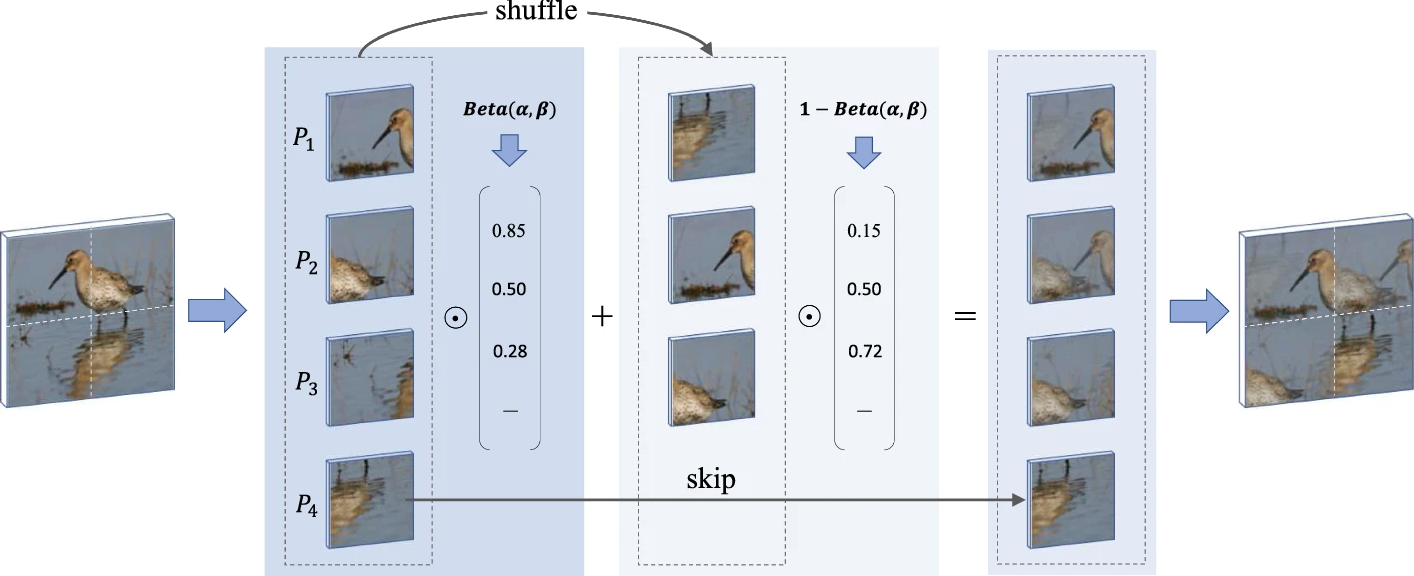
\includegraphics[page=1, width=0.9\textwidth]{./images/patchmix.png}
\caption{PatchMix augmentation. The input image is split into non-overlapping patches, which are shuffled and combined using MixUp-style weights from a Beta distribution. Some patches may bypass mixing for added diversity~\cite{hong2024patchmix}.}
    \label{fig:patchmix}
\end{figure}



Figure~\ref{fig:patchshuffle} presents a simplified version of the PatchShuffle method. In this example, a $4 \times 4$ image matrix is divided into four non-overlapping $2 \times 2$ patches. The pixels within each patch are independently shuffled: attributes in each patch are permutated separately, and a shuffled patch may also have its original structure. This local pixel-level shuffling introduces variation while preserving the global structure of the image~\cite{kang2017patchshuffleregularization}.



\begin{figure}[h!]
    \centering
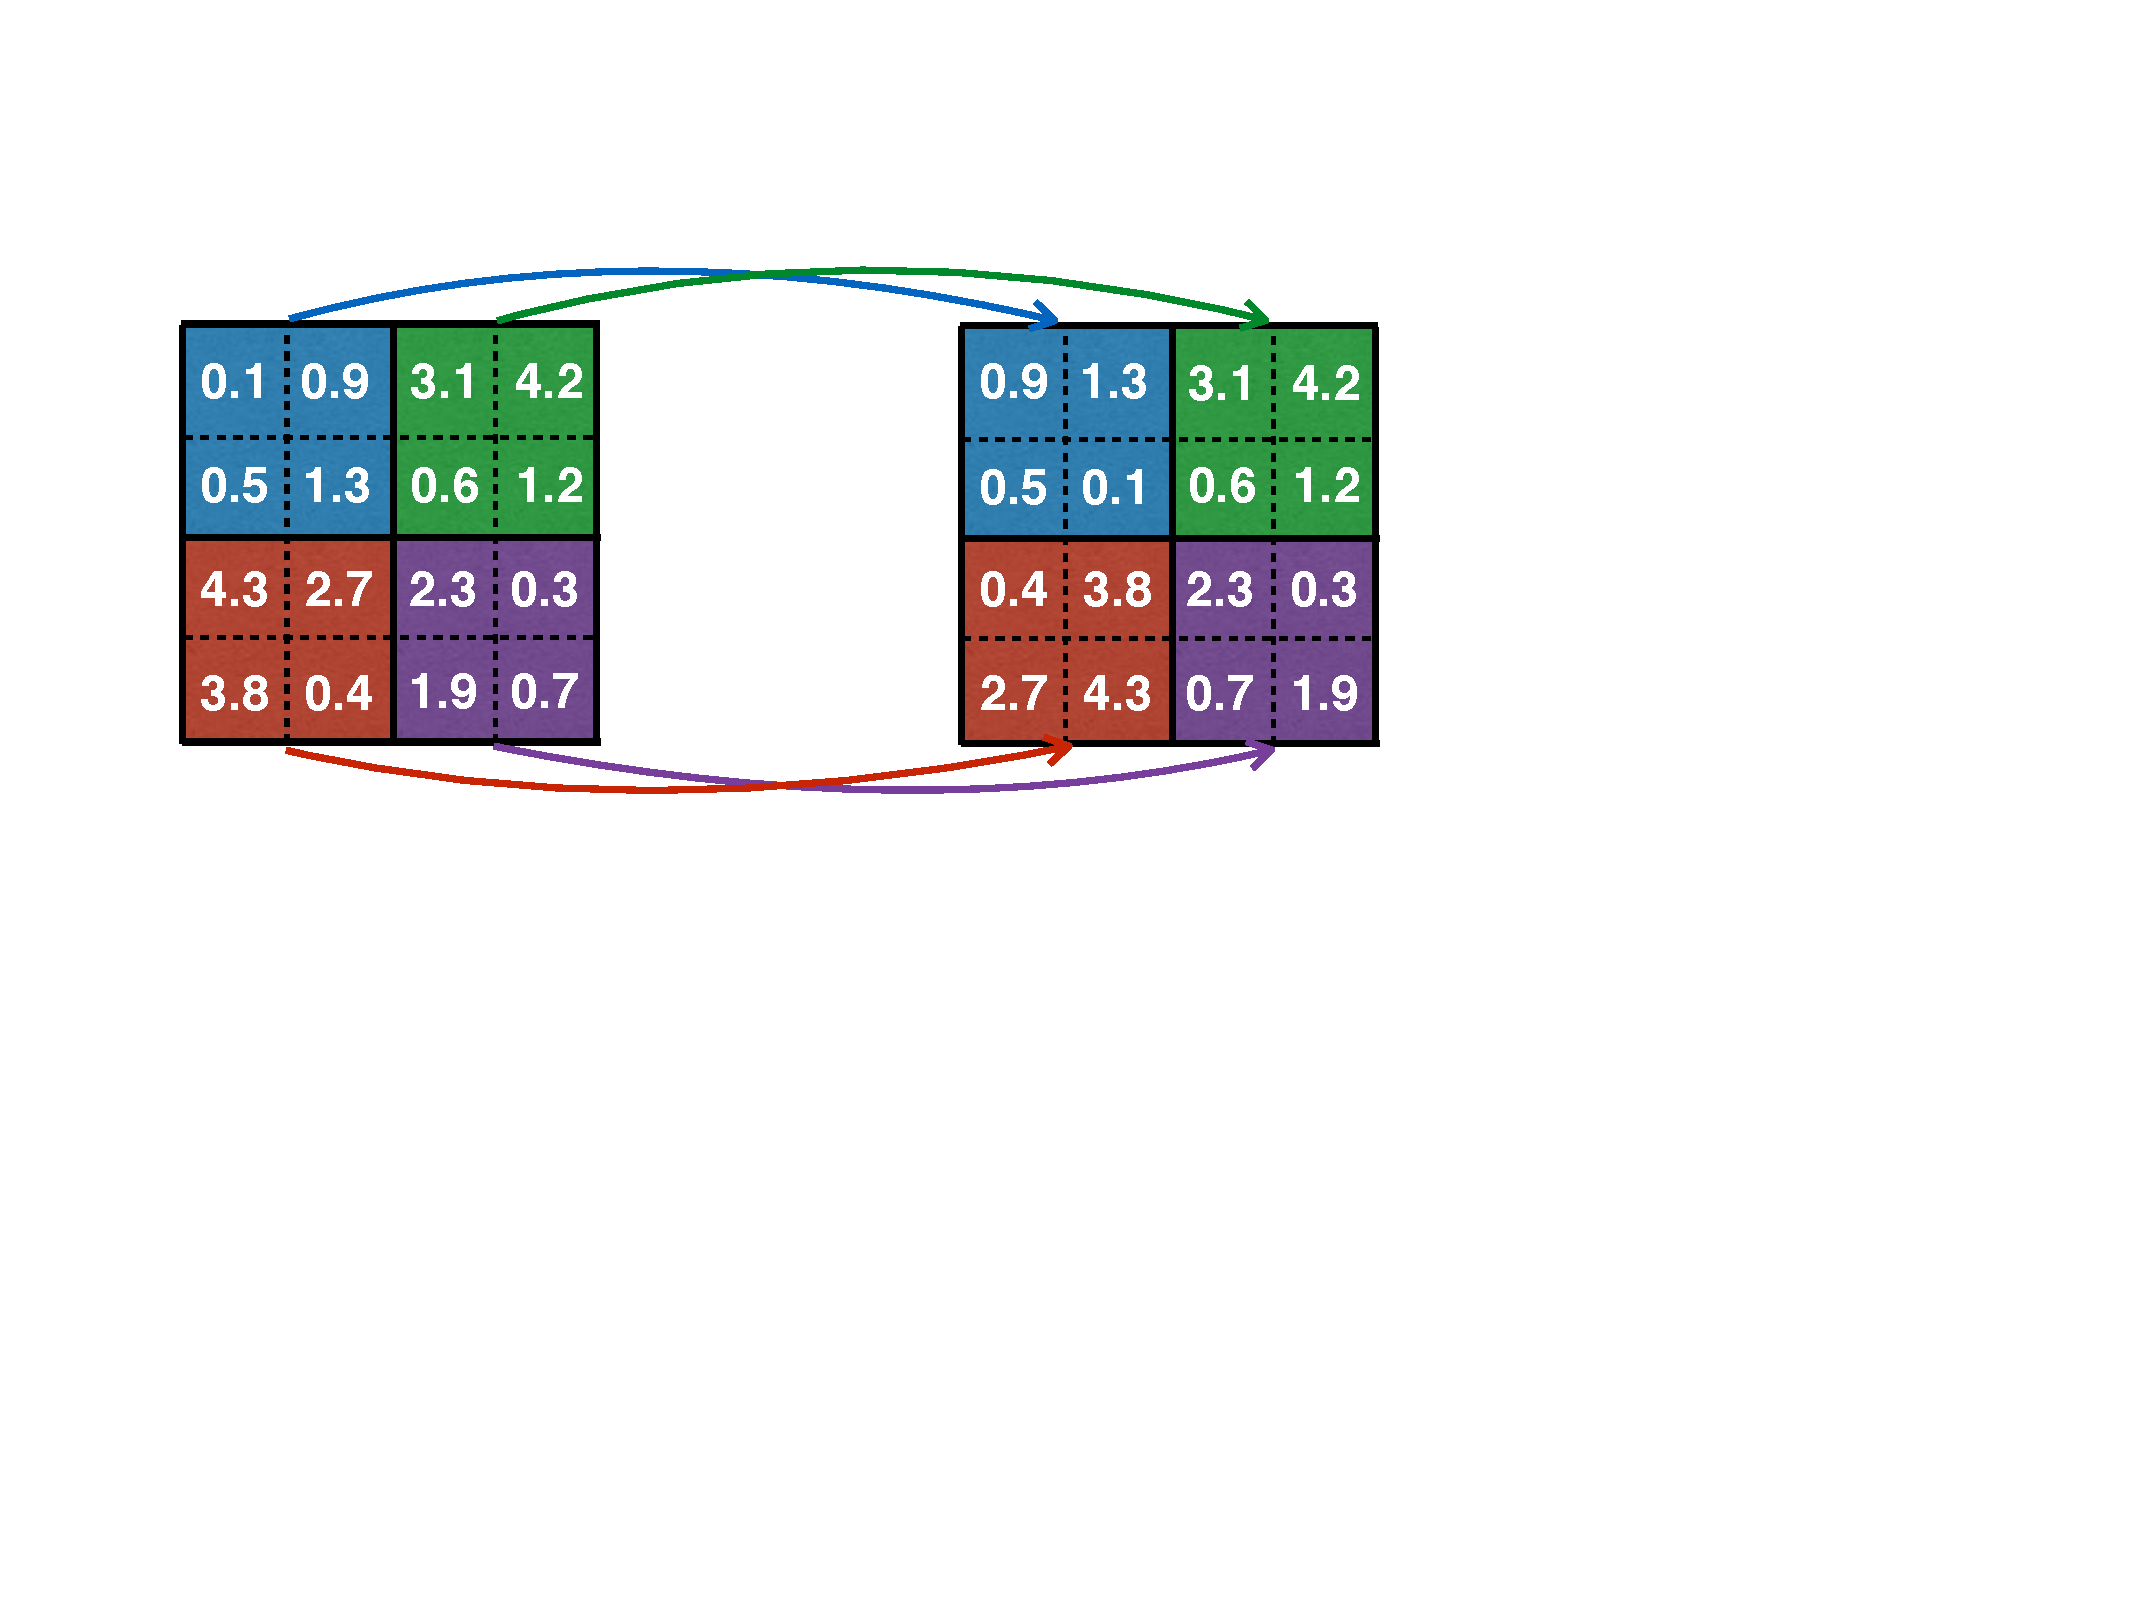
\includegraphics[page=1, width=0.9\textwidth]{./images/PatchShuffle.pdf}
\caption{Simplified illustration of PatchShuffle. A $4 \times 4$ image is split into four $2 \times 2$ patches. Within each patch, pixels are shuffled independently, introducing local variation while preserving the overall image structure~\cite{kang2017patchshuffleregularization}.}
    \label{fig:patchshuffle}
\end{figure}

Figure~\ref{fig:shuffleimages} showcases real-world image samples augmented using PatchShuffle with varying patch sizes. The authors mentioned that PatchShuffle acts as a data augmentation and regularization method. While generated examples maintain the overall global structure of the original input, the internal pixel distributions are altered, making it harder for the model to memorize specific patterns, which is one of the main advantages of the PatchShuffle method. Experimental results demonstrate that PatchShuffle improves classification accuracy and generalization performance across different datasets~\cite{kang2017patchshuffleregularization, hong2024patchmix}.

\begin{figure}[h!]
    \centering
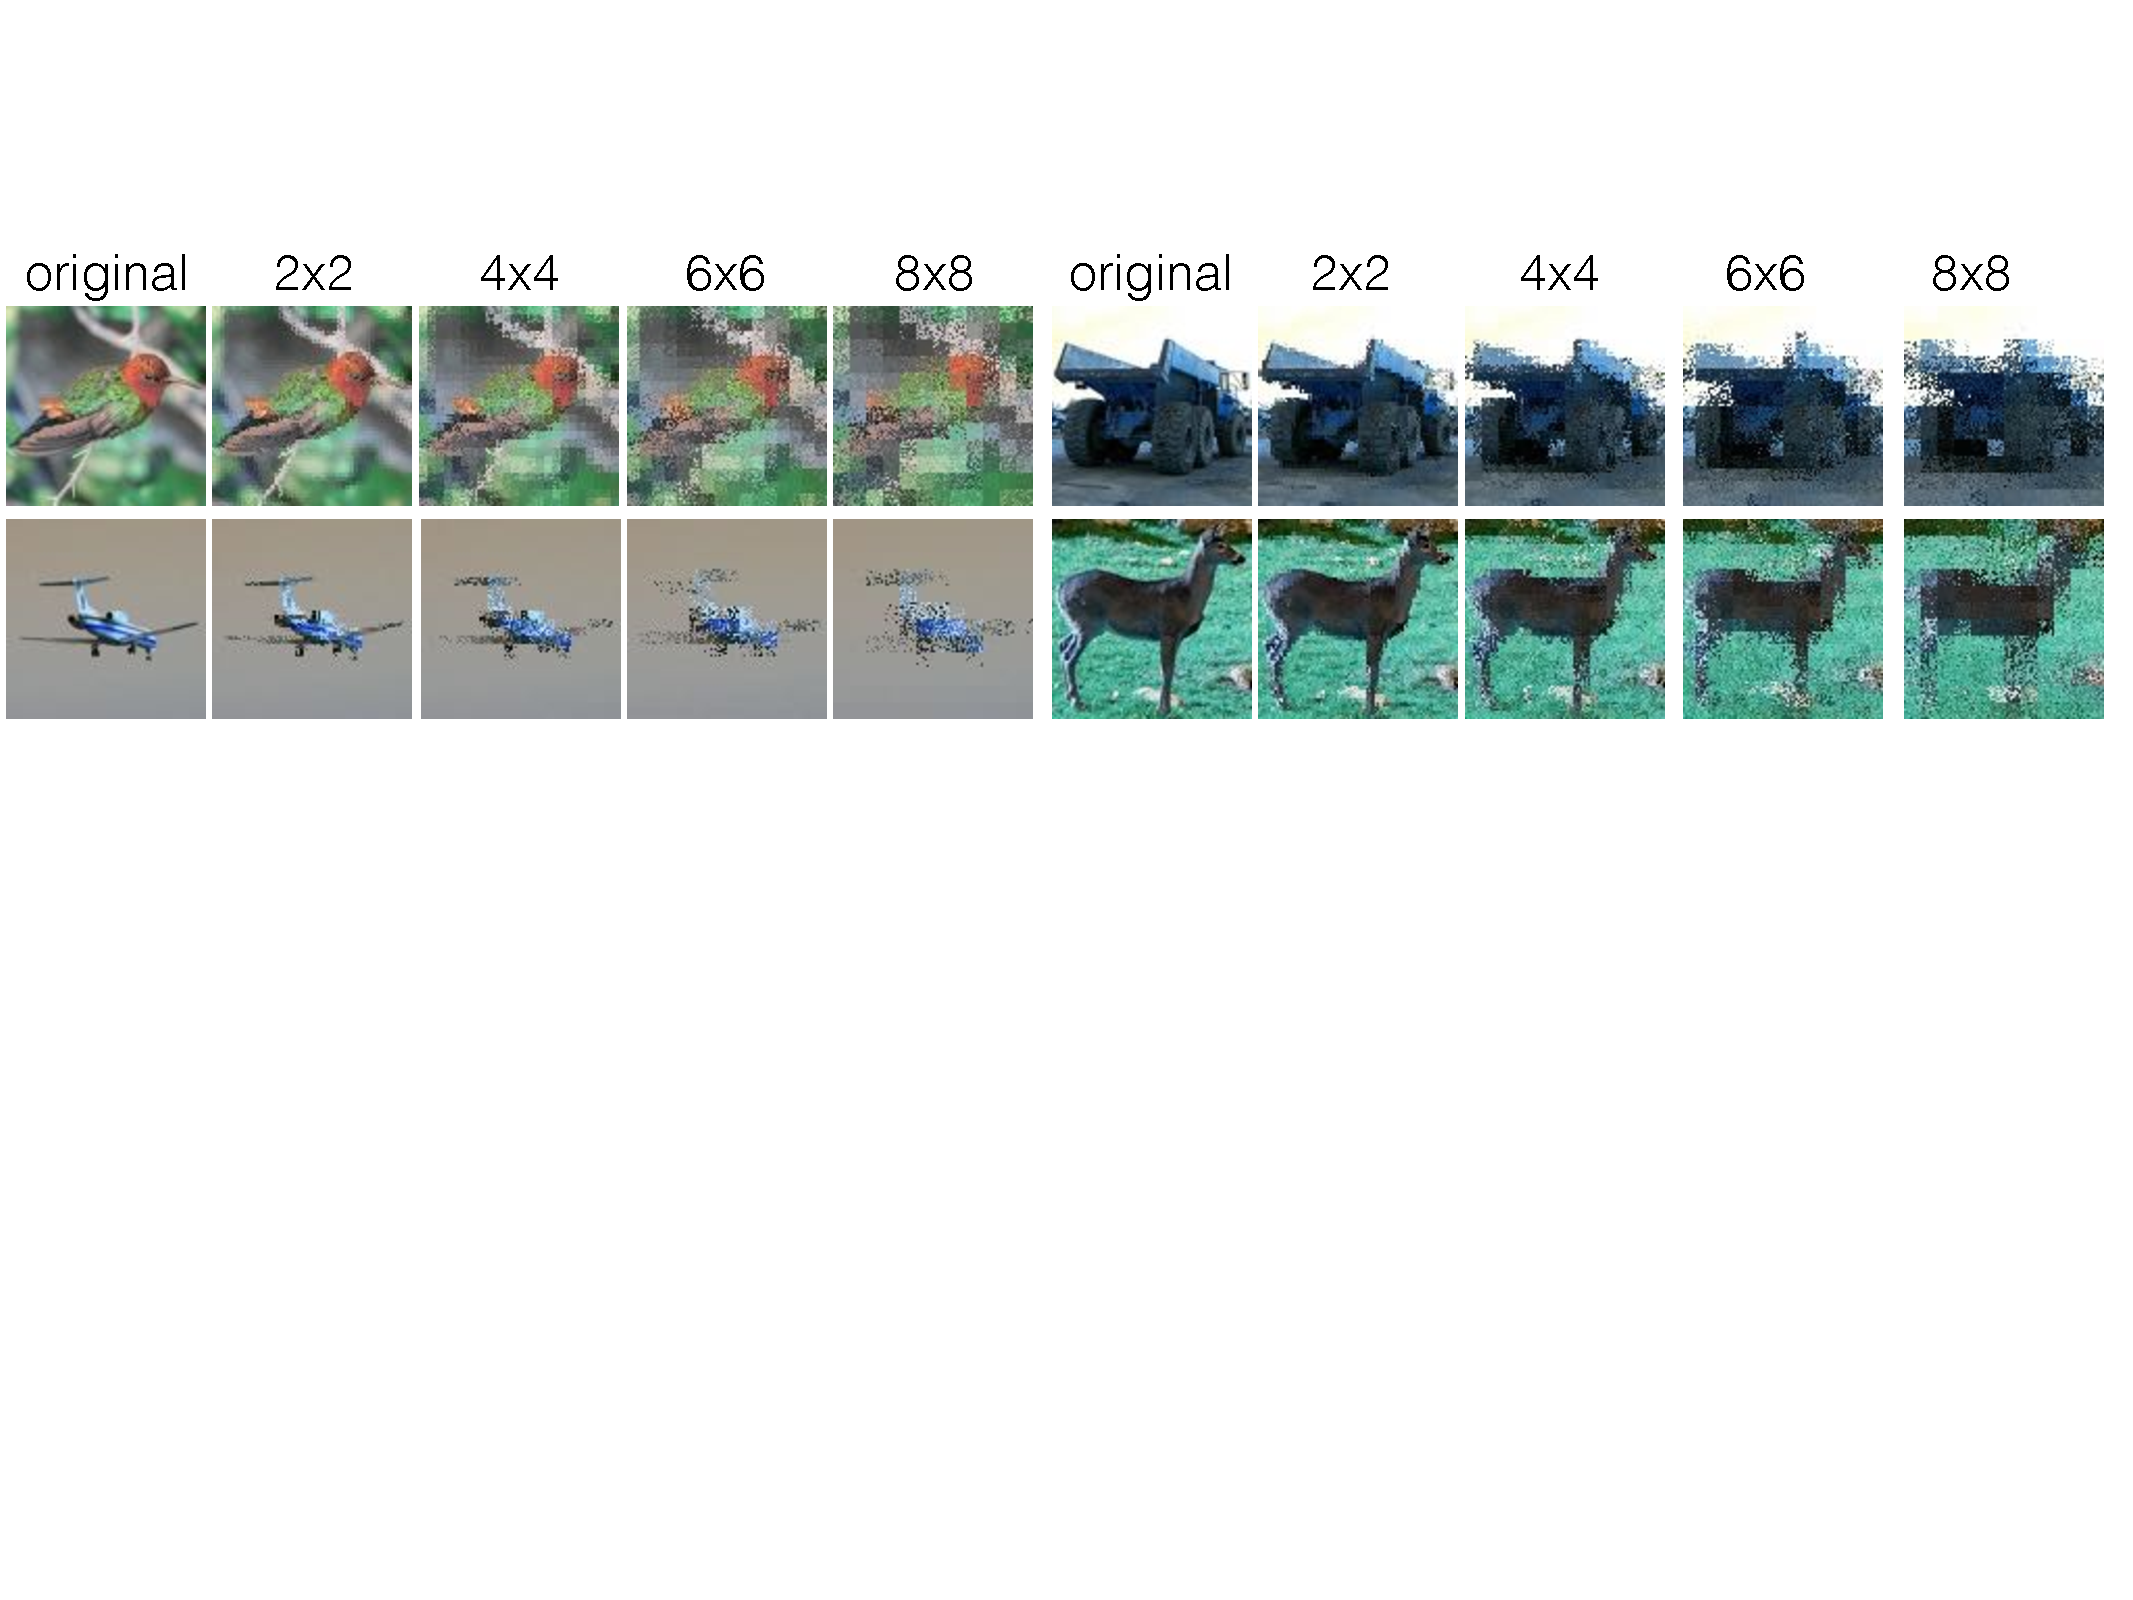
\includegraphics[page=1, width=0.9\textwidth]{./images/ShuffleImages.pdf}
\caption{Real-world image examples augmented with PatchShuffle using different patch sizes. While the global structure is preserved, the internal pixel distribution is altered, promoting regularization and improving generalization by reducing the risk of memorization~\cite{kang2017patchshuffleregularization}.}
    \label{fig:shuffleimages}
\end{figure}



Our proposed method, Temporal Patch Shuffle (TPS), is inspired by patch-based augmentation and regularization techniques developed in the image domain, including PatchShuffle and PatchMix. Nonetheless, applying similar techniques to time series data presents unique challenges. 

Non-overlapping patching and spatial transformations, such as cropping, masking, flipping, etc., are suitable for images as they are structured in a two-dimensional grid. However, they are inappropriate for time series data as they are intrinsically sequential and significantly reliant on temporal order. Transformations such as shuffling or segment reordering can significantly disrupt the temporal dynamics and coherence, potentially worsening performance~\cite{arabi2024wavemaskmixexploringwaveletbasedaugmentations, chen2023fraugfrequencydomainaugmentation}. Our ablation study in Table~\ref{tab:ablation_dlinear} illustrates that using PatchShuffle-style (dividing into non-overlapping patches and shuffling) on time series data results in significantly inferior performance due to the disruption of temporal continuity.

In contrast, our TPS method uses "temporal patches," a concept similarly applied in models like PatchTST~\cite{nie2023timeseriesworth64}, where time series data are partitioned into overlapping segments (patches) with a carefully chosen patch length and stride. These overlapping windows maintain local temporal dependencies and structure to a reasonable degree, even when exposed to transformations such as shuffling. Our ablation study, presented in Figure~\ref{fig:tsne}, utilizes t-distributed Stochastic Neighbor Embedding (t-SNE) visualizations to compare original and augmented samples, supporting our hypothesis that, with appropriately chosen stride and patch length, shuffling patches serves as an effective transformation. It preserves essential signal characteristics while introducing a small amount of functional variability. The results in Table~\ref{tab:dist_metrics} further support these findings.



We propose that this augmentation method, using optimally calibrated parameters, can diminish generalization error, enhance robustness, and reduce variance, similar to the successes of PatchShuffle and PatchMix in image data. Furthermore, we assert that TPS can function as a comprehensive framework for data augmentation within the time series domain. With slight alterations, it can be adapted for various time series tasks, including forecasting and classification.

Sections~\ref{sec: tps_tsf} and \ref{sec:tps_tsc}  describe the specific TPS versions and their applications in time series forecasting and classification, respectively.



\section{TPS for Time Series Forecasting} \label{sec: tps_tsf}



TPS employs the concept of \textit{temporal patches}, where overlapping windows are created using the patch length and stride as hyperparameters within the Temporal Patching block (depicted in green in Figure~\ref{fig:tpstsf}). In the subsequent Variance-Aware Shuffling block (depicted in purple in Figure~\ref{fig:tpstsf}), these patches are sorted in ascending order based on their variance and selectively shuffled according to a predefined \textit{shuffle rate}, $\alpha$. Finally, the augmented sequence is reconstructed by averaging overlapping regions. Before applying the Temporal Patching block, the look-back window and forecast horizon (target) are concatenated like other augmentation methods.

\begin{figure}[h!]
    \centering

\includegraphics[page=1, width=1.0\textwidth, keepaspectratio]{./images/tsf1.drawio.png}
\caption{Illustration of the proposed TPS method for time series forecasting. The input sequence, consisting of a look-back window and a target horizon, is first processed by the \textit{Temporal Patching} block to extract overlapping patches. These patches are then sorted by variance and partially shuffled in the \textit{Variance-Aware Shuffling} block. Finally, the shuffled patches are merged back into a full sequence via the \textit{Reconstruction} block by averaging overlapping regions.}

% {./images/tps_tsf.drawio.png}
    \label{fig:tpstsf}
\end{figure}


Formally, a time series sequence as a combination of look-back window $L$ and forecast horizon $F$ is defined with batch size $B$, sequence length $T$, and number of channels $C$ as:

\begin{equation} \label{eq: concat}
\mathbf{X} = [\mathbf{L}, \mathbf{F}] \in \mathbb{R}^{B \times T \times C}.
\end{equation}


The \textbf{Temporal Patching} block generates patches $\mathbf{P}$ with patch length $p$ and stride $s$ as follows:

\begin{equation} \label{eq: patching}
\mathbf{P} = \text{Unfold}(\mathbf{X}, p, s) \in \mathbb{R}^{B \times N_p \times C \times p},
\end{equation}
where the number of patches $N_p$ is given by:

\begin{equation} 
N_p = \left\lfloor \frac{T - p}{s} + 1 \right\rfloor.
\end{equation}


The \textbf{Unfold} operation extracts patches (sliding windows) from the temporal dimension. The resulting patch tensor is denoted by $\mathbf{P} \in \mathbb{R}^{B \times N_p \times C \times p}$, where $B$ is the batch size, $N_p$ is the number of patches, $C$ is the number of channels, and $p$ is the patch length.

For each sample $b$ in the batch and each patch position $i$, a window of length $p$ is selected starting at temporal position $i \cdot s$ across all channels. This window is then transposed to match the shape $\mathbb{R}^{C \times p}$:
\begin{equation}
\mathbf{P}[b, i] = \left( \mathbf{X}[b, i \cdot s : i \cdot s + p, :] \right)^\top
\end{equation}
This process iterates over all $N_p$ possible patch positions to fill the complete tensor $\mathbf{P}$.


Within the \textbf{Variance-Aware Shuffling} block, importance scores are computed by calculating the variance across the channels and temporal dimension of each patch. For each batch and patch, we first compute the mean across channels and patch temporal elements:
\begin{equation}
\bar{\mathbf{P}}[b, i] = \frac{1}{C \cdot p} \sum_{c=1}^{C} \sum_{j=1}^{p} \mathbf{P}[b, i, c, j]
\end{equation}

Then, the variance is calculated using the correction:
\begin{equation}
\text{Var}(\mathbf{P}[b, i]) = \frac{1}{C \cdot p - 1} \sum_{c=1}^{C} \sum_{j=1}^{p} (\mathbf{P}[b, i, c, j] - \bar{\mathbf{P}}[b, i])^2
\end{equation}

This process generates the importance scores for all patches:
\begin{equation} \label{eq: score}
\text{Score} = \text{Var}(\mathbf{P}) \in \mathbb{R}^{B \times N_p}.
\end{equation}


The number of patches selected for shuffling, $N_s$, is determined by the hyperparameter $\alpha$:

\begin{equation} \label{eq:numberofpatches}
N_s = \left\lfloor \alpha N_p \right\rfloor, \quad \alpha \in (0, 1].
\end{equation}

For each batch, patches are ranked based on their variance scores. Patch indices are sorted, and the indices of the $N_s$ patches with the lowest variance are selected.



\begin{equation} \label{eq: patch_indices}
\mathcal{I} = \{ i_1, i_2, \dots, i_{N_s} \} \subseteq \{1, 2, \dots, N_p\}.
\end{equation}

The selected patches are then randomly shuffled as:

\begin{equation} \label{eq: patchshuffling}
\mathbf{P}_b[\mathcal{I}] = \mathbf{P}_b[\sigma(\mathcal{I})],
\end{equation}
where $\sigma$ denotes a random permutation function applied to the selected indices $\mathcal{I}$.

The \textbf{Reconstruction} block aggregates the shuffled patches by placing each patch back into its original temporal position and averaging overlapping regions. Each patch is positioned according to its stride interval, and when patches overlap due to stride being smaller than patch length, their values are averaged to create a smooth reconstruction. This process generates the final augmented time series: 

\begin{equation}
\mathbf{S} \in \mathbb{R}^{B \times T \times C}.
\end{equation}


$\mathbf{S}$ is partitioned into $\mathbf{S}_L$ and and $\mathbf{S_F}$, where $\mathbf{S_L}$ is concatenated to the original look-back window and $\mathbf{S_F}$ is concatenated to the original target horizon. It follows the same training pipeline as the other augmentations illustrated in Figure~\ref{fig:train_fw}. The pseudocode for TPS is provided in Algorithm~\ref{alg:tps}. 

\begin{algorithm}[H]
\caption{Temporal Patch Shuffle (TPS)}
\label{alg:tps}
\begin{algorithmic}[1]
\REQUIRE Look-back window $\mathbf{L}$ and forecast horizon $\mathbf{F}$, patch length $p$, stride $s$, shuffle rate $\alpha$
\ENSURE Augmented time series $\mathbf{S}$

\STATE $\mathbf{X} \gets \text{Concat}(\mathbf{L}, \mathbf{F})$ \COMMENT{Concatenate input and target sequences}
\STATE $\mathbf{P} \gets \text{Unfold}(\mathbf{X}, p, s)$ \COMMENT{Create overlapping temporal patches}
\STATE $\text{Score} \gets \text{Var}(\mathbf{P})$ \COMMENT{Compute variance-based importance scores}
\STATE $\mathcal{I} \gets \text{Argsort}(\text{Score})[:\alpha \cdot N_p]$ \COMMENT{Select patches with lowest variance}
\STATE $\mathbf{P}[\mathcal{I}] \gets \text{Shuffle}(\mathbf{P}[\mathcal{I}])$ \COMMENT{Shuffle selected patches} \label{alg: shuffle_patches}
\STATE $\mathbf{S} \gets \text{Reconstruct}(\mathbf{P})$ \COMMENT{Reconstruct sequence by averaging overlaps}
\STATE \textbf{return} $\mathbf{S}$
\end{algorithmic}
\end{algorithm}





\section{TPS for Time Series Classification} \label{sec:tps_tsc}


For time series classification, we propose two versions of TPS adapted to the classification setting. Unlike forecasting, where the input consists of both the look-back window and the forecast horizon, classification models only receive the input sequence $\mathbf{X} \in \mathbb{R}^{N \times T \times C}$, where $N$ denotes the number of samples, $T$ the temporal length, and $C$ the number of channels.

The first version of TPS, illustrated in Figure~\ref{fig:tpstsc1}, follows the same procedure as described in Section~\ref{sec: tps_tsf}, with the following modifications:

\begin{itemize}
    \item Instead of concatenating the input and forecast horizon, only the raw input $\mathbf{X}$ without labels is used.
    \item The shuffling process is applied at the \textit{sample level} rather than the batch level; that is, TPS is applied independently to each sample. The batch dimension $B$ is replaced by the sample dimension $N$ in our formulation.
\end{itemize}

For classification, we apply edge-value padding to ensure full patch coverage. This differs from the forecasting setting, where padding is omitted. The pseudocode for this version follows the structure of Algorithm~\ref{alg:tps}, incorporating the modifications listed above.


\begin{figure}[h!]
\centering

\includegraphics[page=1, width=1.0\textwidth, keepaspectratio]{./images/tsctps.png}
\caption{Illustration of the first version of the proposed TPS method for time series classification. This version adapts the forecasting design by applying Temporal Patching and Variance-Aware Shuffling at the sample level, using only the input data without class labels.} 
    \label{fig:tpstsc1}
\end{figure}


The second version, \textbf{Temporal Index Patch Shuffle (TIPS)}, extends TPS by introducing patch-level index shuffling \textit{across samples of the same class}. Rather than reusing patches from the same sample, this version replaces selected patches with patches from other random samples sharing the same class label.

Formally, given labels $Y \in \mathbb{R}^{N}$ or one-hot encoded labels $\mathbf{Y} \in \mathbb{R}^{N \times K}$, for each sample $i$ with label $y_i$, we define the set of other samples with the same label as:

\begin{equation}
\mathcal{N}_i = \left\{ j \in \{1, \dots, N\} \,\middle|\, y_j = y_i,\ j \ne i \right\}.
\end{equation}

For each selected patch index $P_k$ in sample $i$, we randomly select a sample $j \in \mathcal{N}_i$, extract the patch from the same temporal location, and use it to replace the corresponding patch in sample $i$. This replacement is repeated $N_s$ times for each patch that needs to be shuffled. The procedure introduces semantic diversity while preserving class consistency. To maintain dimensional consistency, edge-value padding is applied when necessary. An illustration of this process is provided in Figure~\ref{fig:tpstsc2}.



\begin{figure}[h!]
    \centering
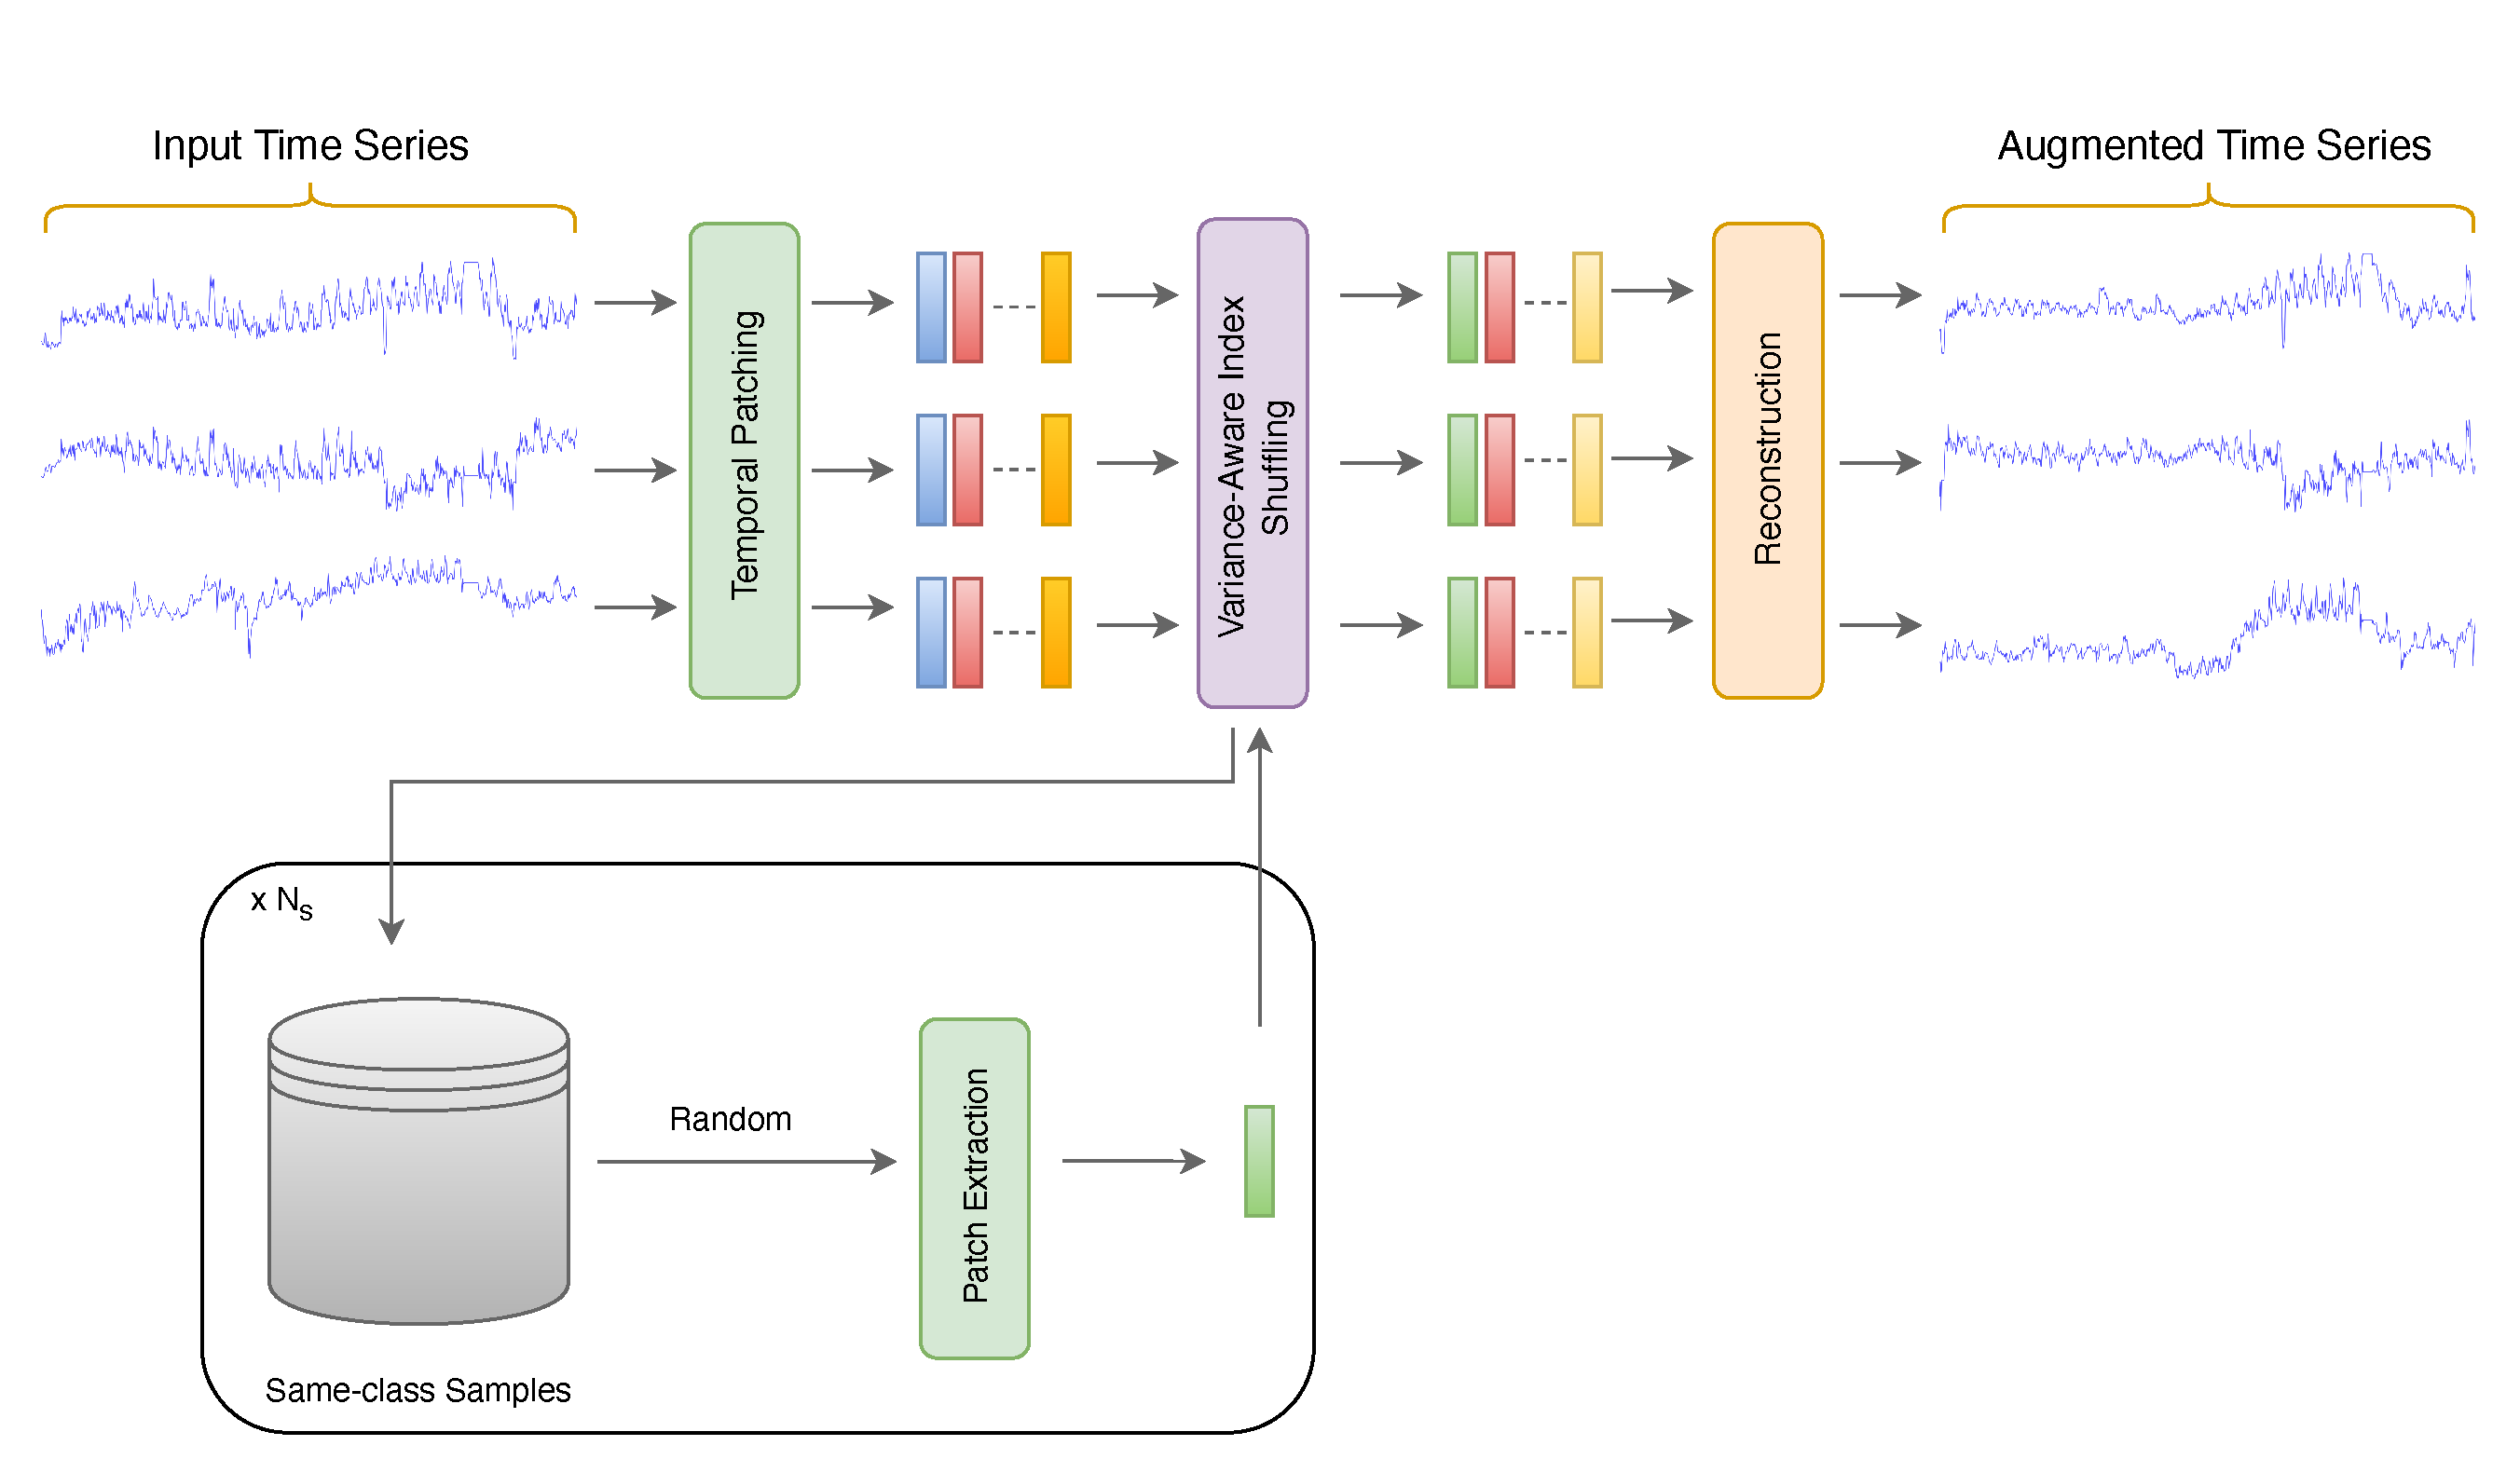
\includegraphics[page=1, width=1.0\textwidth, keepaspectratio]{./images/tps_tsc.drawio2.drawio.pdf}
\caption{Illustration of the second version of the proposed method, \textbf{Temporal Index Patch Shuffle (TIPS)}, for time series classification. Unlike the first version of TPS, TIPS introduces patch-level shuffling \emph{across samples with the same class label}. For each selected patch within a sample, TIPS replaces it with a patch from the same temporal location of a randomly selected sample belonging to the same class}

    \label{fig:tpstsc2}
\end{figure}

The pseudocode for TIPS is presented in Algorithm~\ref{alg:tps_class}. The key difference from the original version lies in Lines~\ref{alg: same-class}–\ref{alg: cross_patch}, which implement an additional step: extracting patches from a randomly selected sample belonging to the same class as the current instance (illustrated in Figure~\ref{fig:tpstsc2}). In contrast, the original version (Algorithm~\ref{alg:tps}) uses a simpler shuffling operation, represented by Line~\ref{alg: shuffle_patches}, without involving any cross-sample interactions. It is also important to note that, in practice, all operations for the classification setting are applied in a per-sample sequential manner. These two versions for classification tasks follow the training pipeline in Figure~\ref{fig:tsc_fw}, the same as other augmentation methods.



\begin{algorithm}[H]
\caption{Temporal Index Patch Shuffle (TIPS)}
\label{alg:tps_class}
\begin{algorithmic}[1]
\REQUIRE Input sequence $\mathbf{X} \in \mathbb{R}^{N \times T \times C}$, labels $Y \in \mathbb{R}^N$, patch length $p$, stride $s$, shuffle rate $\alpha$
\ENSURE Augmented time series $\mathbf{S} \in \mathbb{R}^{N \times T \times C}$

\STATE $\mathbf{P} \gets \text{Unfold}(\mathbf{X}, p, s)$ \COMMENT{Create overlapping patches for each sample}
\STATE $\text{Score} \gets \text{Var}(\mathbf{P})$ \COMMENT{Compute variance-based scores per sample}
\STATE $N_s \gets \lfloor \alpha \cdot N_p \rfloor$ \COMMENT{Determine number of patches to shuffle per sample}

\FOR{each sample $i \in \{1, \dots, N\}$}
    \STATE $\mathcal{I}_i \gets \text{Argsort}(\text{Score}_i)[:N_s]$ \COMMENT{Select low-variance patch indices}
    \STATE $\mathcal{N}_i \gets \{ j \in \{1, \dots, N\} \mid y_j = y_i,\ j \ne i \}$ \COMMENT{Find same-class neighbors} \label{alg: same-class}
    \FOR{each index $k \in \mathcal{I}_i$}
        \STATE $j \gets \text{RandomSample}(\mathcal{N}_i)$ \COMMENT{Randomly select same-class sample}
        \STATE $\mathbf{P}_i[k] \gets \mathbf{P}_j[k]$ \COMMENT{Replace patch from same temporal location} \label{alg: cross_patch}
    \ENDFOR
\ENDFOR

\STATE $\mathbf{S} \gets \text{Reconstruct}(\mathbf{P})$ \COMMENT{Reconstruct sequence by averaging overlaps}
\STATE \textbf{return} $\mathbf{S}$
\end{algorithmic}
\end{algorithm}



TPS can be applied to other time series domains with minimal adaptation to task-specific properties. One example is self-supervised models, which typically rely on other augmentations to improve accuracy or reduce errors. We will discuss this in more detail in Section~\ref{sec:future}.


\section{Methodological Rationale \& Design Objectives} \label{sec:method_design}

The design of our proposed method, \textbf{TPS (Temporal Patch Shuffle)}, is grounded in three key objectives: (1) preserving temporal coherence, (2) introducing controlled variability, and (3) maintaining data-label consistency. Unlike image data, time series are highly sensitive to temporal ordering; thus, transformations must avoid disrupting sequential structure.

TPS introduces three tunable parameters—patch length, stride, and shuffle rate—that allow users to flexibly generate either samples closely resembling the original data or augmented sequences with meaningful variability. This facilitates both improved generalization and reduced overfitting. Our ablation studies in Chapter~\ref{chapter:experiments} (see Figure~\ref{fig:tsne} and Table~\ref{tab:dist_metrics}) empirically support these claims.

One component of TPS is \textbf{low-variance patch sorting}, which prioritizes the shuffling of patches with low temporal variability, as they are less critical to the sequence’s temporal structure. In contrast, random selection may disrupt meaningful patterns, particularly in certain datasets and prediction lengths where the shuffle rate is not 1.0. Moreover, the use of \textbf{overlapping patches}—as also utilized in models like PatchTST~\cite{nie2023timeseriesworth64}—helps preserve local dependencies better than non-overlapping alternatives. The final step of \textbf{reconstruction} acts as an implicit smoothing or denoising process, where overlapping regions are averaged to restore the sequence. All of these aspects will be discussed in detail in Section~\ref{sec:ablation}.

In the classification context, we introduce \textbf{TIPS (Temporal Index Patch Shuffle)} as an extension of TPS. This version incorporates \textbf{cross-sample patch exchange} by replacing selected patches with those from other samples within the same class. This is feasible for classification, as samples from the same class can share structural information; however, it is inapplicable to forecasting due to the nature of prediction targets. As demonstrated in Chapter~\ref{chapter:experiments}, TIPS achieves superior performance in both univariate and multivariate classification, outperforming even the original TPS. This highlights the flexibility of our framework: with minimal modifications, it can be adapted for different tasks and objectives.

Both TPS and TIPS are designed to be lightweight and scalable. The primary computational cost stems from patch extraction and shuffling. Since these operations are non-parametric, they can be efficiently integrated into the training pipeline as \textbf{on-the-fly augmentations}, adding minimal overhead in training time or memory usage. To quantify this, we present runtime comparisons for augmentation in Tables~\ref{tab:augmentation_comparison} and \ref{tab:aug_times_tsc}, which focus on forecasting and classification, respectively.

One limitation of TPS and TIPS is the requirement to tune three hyperparameters to match the characteristics of a given dataset. However, according to Figure~\ref{fig:ablation_lightts} in the ablation study, a higher shuffle ratio, moderate patch length, and lower strides generally lead to lower generalization error, which can help us reduce our hyperparameter search cost. In Section~\ref{sec:future}, we explore adaptive patch sizing and other potential enhancements to TPS.

Overall, we have thoroughly evaluated both TPS and TIPS across various models and scenarios in the next chapter. Our ablation studies validate the effectiveness of the proposed design principles. 






% %%%%%%%%%%%%%%%%%%%%%%%%%%%%%%%%%%%%%%%%%
 %!TEX root = ../Master_template.tex
\chapter{Experiments}
\label{chapter:experiments}

In this chapter, we describe the datasets used for all experiments in both time series forecasting and classification (see Section~\ref{sec:datasets}). The experimental setup—including the models, their parameters, hyperparameter configurations, and the tuning of augmentation methods for both forecasting and classification—is detailed in Section~\ref{sec:experimental_setup}. Section~\ref{sec:main_results} presents the main results for long-term and short-term forecasting, as well as univariate and multivariate time series classification. Finally, Section~\ref{sec:ablation} provides various ablation studies related to our proposed methods, covering both forecasting and classification tasks.

\section{Datasets} \label{sec:datasets}

\subsection*{Time Series Forecasting} \label{subsec:dataset-tsf}


We utilize seven benchmark datasets for long-term time series forecasting and four datasets for short-term forecasting tasks. A summary of these datasets is provided in Table~\ref{tab:datasets}. Datasets ranging from ETTh1 to Influenza-like Illness (ILI) are employed for long-term forecasting, while all Caltrans Performance Measurement System (PeMS) datasets are used for short-term forecasting. These datasets span diverse domains and dimensionalities, enabling a comprehensive evaluation of the effectiveness and generalizability of our proposed augmentation method.
The Electricity Transformer Temperature (ETT) datasets~\cite{zhou2021informerefficienttransformerlong} consist of seven variables recorded from electricity transformers, covering the period from July 2016 to July 2018. The ETT datasets are divided into four subsets: ETTh1 and ETTh2, recorded at hourly intervals, and ETTm1 and ETTm2, recorded every 15 minutes.
The Exchange dataset~\cite{wu2022autoformerdecompositiontransformersautocorrelation} contains daily exchange rates from eight countries between 1990 and 2016. The Weather dataset~\cite{wu2022autoformerdecompositiontransformersautocorrelation} includes 21 meteorological variables measured every 10 minutes at the Max Planck Institute for Biogeochemistry Weather Station throughout 2020. We note that experiments were not conducted on the Electricity Consuming Load (ECL), Traffic, Solar-Energy~\cite{lai2018modelinglongshorttermtemporal} due to their substantially higher computational demands (i.e., increased GPU memory and extended training times), which exceeded the available resources for this study.
For short-term forecasting, we utilize the PeMS datasets, which consist of publicly available traffic sensor data collected across California at 5-minute intervals. We adopt four subsets—PeMS03, PeMS04, PeMS07, and PeMS08—as standardized in the SCINet framework~\cite{liu2022scinettimeseriesmodeling}. Table~\ref{tab:datasets} summarizes the input dimensionality, prediction lengths, and dataset sizes for training, validation, and test splits.

\begin{table}[h!]
\vspace{0.5cm}
\centering
\scriptsize
\renewcommand{\arraystretch}{1.2}
\setlength{\tabcolsep}{8pt}
\begin{tabular}{lcccc}
\toprule
\textbf{Dataset} & \textbf{Dim.} & \textbf{Prediction Length} & \textbf{Dataset Size} & \textbf{Information} \\
\midrule
ETTh1 & 7 & \{96, 192, 336, 720\} & (8545, 2881, 2881) & Electricity (Hourly) \\
ETTh2 & 7 & \{96, 192, 336, 720\} & (8545, 2881, 2881) & Electricity (Hourly) \\
ETTm1 & 7 & \{96, 192, 336, 720\} & (34465, 11521, 11521) & Electricity (15min) \\
ETTm2 & 7 & \{96, 192, 336, 720\} & (34465, 11521, 11521) & Electricity (15min) \\
Exchange & 8 & \{96, 192, 336, 720\} & (5120, 665, 1422) & Economy (Daily) \\
Weather & 21 & \{96, 192, 336, 720\} & (36792, 5271, 10540) & Weather (10min) \\
ILI & 7 & \{24, 36, 48, 60\} & (629, 98, 194) & Illness (Weekly) \\
PeMS03 & 358 & \{12, 24, 36, 48\} & (15617, 5135, 5135) & Transportation (5min) \\
PeMS04 & 307 & \{12, 24, 36, 48\} & (10172, 3375, 3375) & Transportation (5min) \\
PeMS07 & 883 & \{12, 24, 36, 48\} & (16911, 5622, 5622) & Transportation (5min) \\
PeMS08 & 170 & \{12, 24, 36, 48\} & (10690, 3548, 3548) & Transportation (5min) \\
\bottomrule
\end{tabular}
\caption{Summary of the datasets used in time series forecasting experiments. The table includes input dimensionality (number of channels), prediction lengths, and dataset sizes for training, validation, and test splits. The datasets span a variety of domains (e.g., electricity, weather, transportation, health) and temporal granularities, supporting both long-term and short-term forecasting tasks~\cite{liu2024itransformerinvertedtransformerseffective}.}
\label{tab:datasets}
\end{table}





\subsection*{Time Series Classification} \label{subsec:datasets-tsc}


We utilize the widely used UCR~\cite{UCRArchive2018} and UEA~\cite{bagnall2018ueamultivariatetimeseries} repositories to evaluate our methodology in univariate and multivariate time series classification tasks.

The UCR archive is extensively utilized within the time series research community and contains solely univariate datasets, each featuring a singular time-dependent variable (i.e., one channel). It is divided into different categories: Device, ECG, Image, Motion, Sensor, Spectrograph, Simulated, and others~\cite{UCRArchive2018}. For our assessment, we chose a varied subset of 128 datasets by incorporating representative samples from different categories. The datasets exhibit variation in training/test sizes, sequence lengths, and output class numbers, making the evaluation extensive and comprehensive. Table~\ref{tab:tsc_datasets} shows the main characteristics of the chosen UCR datasets used in our experiments.




\begin{table}[h!]
\centering
\vspace{0.2cm}
\begin{adjustbox}{max width=\textwidth}
\begin{tabular}{llcccc}
\toprule
\textbf{Type} & \textbf{Dataset} & \textbf{Train Size} & \textbf{Test Size} & \textbf{Length} & \textbf{No. of Classes} \\
\midrule
\multirow{3}{*}{\textbf{Device}} 
& ACSF1 & 100 & 100 & 1460 & 10 \\
& HouseTwenty & 34 & 101 & 3000 & 2 \\
& ScreenType & 375 & 375 & 720 & 3 \\
\midrule
\multirow{3}{*}{\textbf{ECG}} 
& ECG5000 & 500 & 4500 & 140 & 5 \\
& ECG200 & 100 & 100 & 96 & 2 \\
& ECGFiveDays & 23 & 861 & 136 & 2 \\
\midrule
\multirow{7}{*}{\textbf{Image}} 
& Adiac & 390 & 391 & 176 & 37  \\
& FaceFour & 24 & 88 & 350 & 4  \\
& FaceAll & 560 & 1690 & 131 & 14 \\
& HandOutlines & 1000 & 370 & 2709 & 2 \\
& MiddlePhalanxTW & 399 & 154 & 80 & 6 \\
& PhalangesOutlinesCorrect & 1800 & 858 & 80 & 2 \\
& ShapesAll & 600 & 600 & 512 & 60 \\
\midrule
\multirow{3}{*}{\textbf{Motion}} 
& Haptics & 155 & 308 & 1092 & 5 \\
& WormsTwoClass & 181 & 77 & 900 & 2  \\
& InlineSkate & 100 & 550 & 1882 & 7  \\
\midrule
\multirow{7}{*}{\textbf{Sensor}} 
& Car & 60 & 60 & 577 & 4 \\
& Earthquakes & 322 & 139 & 512 & 2 \\
& FordA & 3601 & 1320 & 500 & 2  \\
& FordB & 3636 & 810 & 500 & 2  \\
& ItalyPowerDemand & 67 & 1029 & 24 & 2  \\
& Lightning2 & 60 & 61 & 637 & 2  \\
& StarLightCurves & 1000 & 8236 & 1024 & 3  \\
\midrule
\multirow{5}{*}{\textbf{Spectro}} 
& Beef & 30 & 30 & 470 & 5  \\
& EthanolLevel & 504 & 500 & 1751 & 4  \\
& Wine & 57 & 54 & 234 & 2  \\
& Meat & 60 & 60 & 448 & 3 \\
& OliveOil & 30 & 30 & 570 & 4  \\
\midrule
\multirow{2}{*}{\textbf{Simulated \& Audio}} 
& ChlorineConcentration & 467 & 3840 & 166 & 3 \\
& Phoneme & 214 & 1896 & 1024 & 39 \\
\bottomrule
\end{tabular}
\end{adjustbox}
\caption{Summary of selected UCR univariate time series classification datasets used in our experiments. The table includes dataset category, name, training and test set sizes, input sequence lengths, and number of output classes~\cite{UCRArchive2018}.}
\label{tab:tsc_datasets}
\end{table}

In contrast, the UEA archive pertains to multivariate time series classification tasks. The datasets consist of various channels with input features varying from 2 to 1345~\cite{bagnall2018ueamultivariatetimeseries}. We selected 10 datasets from the 30 in the UEA archive representing diverse characteristics, covering multiple application domains and varying dimensionality. Table~\ref{tab:tsc_multivariate} provides detailed information about the chosen UEA datasets, including their sizes, sequence lengths, dimensionality, and number of output classes.




\begin{table}[h!]
\centering
\begin{adjustbox}{max width=\textwidth}
\begin{tabular}{lccccc}
\toprule
\textbf{Dataset} & \textbf{Train Size} & \textbf{Test Size} & \textbf{Dimensions} & \textbf{Length} & \textbf{No. of Classes} \\
\midrule
AtrialFibrillation & 15 & 15 & 2 & 640 & 3 \\
Cricket & 108 & 72 & 6 & 1197 & 12 \\
DuckDuckGeese & 60 & 40 & 1345 & 270 & 5 \\
ERing & 30 & 30 & 4 & 65 & 6 \\
EthanolConcentration & 261 & 263 & 3 & 1751 & 4 \\
LSST & 2459 & 2466 & 6 & 36 & 14 \\
Libras & 180 & 180 & 2 & 45 & 15 \\
FaceDetection & 5890 & 3524 & 144 & 62 & 2 \\
FingerMovements & 316 & 100 & 28 & 50 & 2 \\
MotorImagery & 278 & 100 & 64 & 3000 & 2 \\
\bottomrule
\end{tabular}
\end{adjustbox}
\caption{Characteristics of the multivariate time series classification datasets selected from the UEA archive. These datasets span a wide range of application domains and vary significantly in input dimensionality, sequence length, and number of classes, offering a robust benchmark for evaluating model performance on multivariate data~\cite{bagnall2018ueamultivariatetimeseries}.}
\label{tab:tsc_multivariate}
\end{table}

The UCR and UEA repositories are standard benchmarks in time series classification literature and are frequently employed in comparative studies~\cite{UCRArchive2018, bagnall2018ueamultivariatetimeseries}. Our evaluation achieves broad applicability through experimentation on datasets from both repositories and ensures comparable results. 


\section{Experimental Setup} \label{sec:experimental_setup}

\subsection*{Time Series Forecasting} \label{subsec:experimental_setup-tsf}


We utilize five distinct models for long-term forecasting tasks, encompassing linear architectures with multi-layer perceptrons (MLPs) and Transformer-based frameworks. This selection allows an in-depth evaluation of the effectiveness of our augmentation method across various modeling frameworks.

PatchTST~\cite{nie2023timeseriesworth64} is an efficient Transformer-based model that partitions time series into segments, treating these segments as input tokens for the Transformer. In addition, PatchTST employs a channel-independent architecture, facilitating the efficient modeling of temporal dependencies across distinct features~\cite{nie2023timeseriesworth64}.

DLinear~\cite{zeng2022transformerseffectivetimeseries} demonstrates a completely linear methodology, wherein the authors illustrated that even basic, single-layer linear models could surpass some Transformer-based architectures in long-term forecasting tasks.

TSMixer~\cite{chen2023tsmixerallmlparchitecturetime} is a model formed by stacked multi-layer perceptrons (MLPs). It successfully integrates information across temporal and feature dimensions via MLP operations, providing a highly scalable and straightforward alternative to traditional sequence models~\cite{chen2023tsmixerallmlparchitecturetime}.

Time-series Dense Encoder (TiDE)~\cite{das2024longtermforecastingtidetimeseries} follows an encoder-decoder design based entirely on MLPs. It can model non-linear dependencies and effectively handle covariates, making it particularly suitable for more complex forecasting settings~\cite{das2024longtermforecastingtidetimeseries}.


LightTS~\cite{zhang2022morefastmultivariatetime} is a lightweight deep learning model combining MLP-based processing with two down-sampling strategies: interval and continuous. This design reduces computational complexity while preserving essential temporal information~\cite{zhang2022morefastmultivariatetime}.


Applying these models guarantees that our experimental evaluation covers a broad spectrum of architectures with various modeling assumptions and complexities. This enables a comprehensive evaluation of the robustness and effectiveness of our proposed augmentation method.


Ultimately, while our emphasis is on linear, MLP-based, and Transformer-based models, we will address the prospective application of our methodology to graph neural networks (GNNs) and recurrent neural networks (RNNs) in future work (see Section~\ref{sec:future}).

The input sequence lengths are chosen according to the optimal configurations reported in the original studies, as our aim is to evaluate augmentation techniques under optimal model conditions fairly. During training, we configured the number of epochs to 20 (except that it is less than 20 in the original configuration), employing early stopping with the patience of 10 epochs and saving the model weights, which resulted in the lowest validation loss. Despite certain original studies indicating training for 100 epochs or more, we limit the training to fewer due to computational constraints. However, this change only results in minor inconsistencies relative to the initial findings and does not affect the overall conclusions.

Learning rate schedulers are chosen according to the recommendations of the original papers when available or alternatively based on our empirical evaluation to ensure stable convergence. Learning rates are calibrated either based on the initial configurations or through validation-driven adjustments.

The input sequence lengths are set as follows:


\begin{itemize}
    \item For DLinear and PatchTST, the input sequence length is 336.
    \item For TiDE and LightTS, it is 720.
    \item For TSMixer, the input sequence length is 512.
\end{itemize}

For specific datasets, such as ILI, the sequence length is reduced to 104, following the guidelines from the corresponding papers and confirmed by our own evaluation. This adjustment is necessary because these datasets contain relatively few temporal points, making longer input sequences impractical~\cite{zeng2022transformerseffectivetimeseries, nie2023timeseriesworth64}.

By carefully adjusting input lengths, learning rates, and schedulers by best practices, we ensure that our augmentation method is assessed under fair and competitive conditions across all baseline models.



We optimized the hyperparameters of several augmentation techniques, including FreqAdd, FreqPool, Upsample, Frequency Masking (FreqMask), Frequency Mixing (FreqMix), Dominant Shuffle, and our proposed method, Temporal Patch Shuffle (TPS), on the ETTh1, ETTh2, ETTm1, and ETTm2 datasets using the TSMixer model. Due to computational constraints, we did not perform hyperparameter tuning for methods such as weighted Dynamic Time Warping Barycentric Averaging (wDBA), Moving Block Bootstrapping (MBB), RobustTAD,  Spectral and Time Augmentation (STAug), wavelet masking (WaveMask), and wavelet mixing (WaveMix).
Table~\ref{tab:aug_params} outlines the key hyperparameters associated with each augmentation method. RobustTAD-m/p indicates that the RobustTAD method has been applied either to the magnitude or the phase component. For our method TPS, we evaluated 25 distinct configurations (see Table~\ref{tab:tps_parameters_split1}). Each configuration was run five times, and the optimal setting was selected based on the validation loss, while also considering the standard deviation to ensure robustness.

\begin{table}[h!]
\centering
\begin{tabular}{@{}ll@{}}
\toprule
\textbf{Method} & \textbf{Parameters} \\
\midrule
wDBA              & weighting, DTW constraints \\
MBB               & block size, STL period \\
RobustTAD-m/p     & perturbation rate, number of segments, segment length \\
FreqAdd           & perturbation rate \\
FreqPool          & pool size \\
Upsample          & subsequence length rate \\
STAug             & mixup rate \\
FreqMask          & masking rate \\
FreqMix           & mixing rate \\
WaveMix \& WaveMask      & wavelet type, decomposition level, sampling rate \\
Dominant Shuffle  & shuffle rate \\
TPS               & patch length, stride, shuffle rate \\
\bottomrule
\end{tabular}
\caption{Hyperparameters used for each time series forecasting augmentation method.}

\label{tab:aug_params}
\end{table}



\begin{table}[h!]
\centering
\begin{minipage}[t]{0.48\linewidth}
\centering
\begin{tabular}{@{}cccc@{}}
\toprule
\# & $p$ & $s$ & $\alpha$ \\
\midrule
1  & 16  & 5   & 0.8 \\
2  & 16  & 12  & 0.9 \\
3  & 16  & 1   & 1.0 \\
4  & 32  & 5   & 1.0 \\
5  & 32  & 8   & 0.9 \\
6  & 32  & 8   & 1.0 \\
7  & 32  & 12  & 0.7 \\
8  & 32  & 16  & 1.0 \\
9  & 64  & 2   & 1.0 \\
10 & 72  & 24  & 1.0 \\
11 & 96  & 2   & 1.0 \\
12 & 96  & 16  & 0.7 \\
13 & 96  & 32  & 0.9 \\
\bottomrule
\end{tabular}
\end{minipage}
\hfill
\begin{minipage}[t]{0.48\linewidth}
\centering
\begin{tabular}{@{}cccc@{}}
\toprule
\# & $p$ & $s$ & $\alpha$ \\
\midrule
14 & 96  & 96  & 1.0 \\
15 & 120 & 12  & 0.9 \\
16 & 120 & 12  & 1.0 \\
17 & 120 & 24  & 1.0 \\
18 & 120 & 36  & 1.0 \\
19 & 120 & 1   & 1.0 \\
20 & 168 & 24  & 0.8 \\
21 & 192 & 12  & 0.8 \\
22 & 200 & 24  & 1.0 \\
23 & 220 & 8   & 1.0 \\
24 & 240 & 24  & 0.8 \\
25 & 240 & 24  & 1.0 \\
\bottomrule
\end{tabular}
\end{minipage}
\caption{Hyperparameter configurations used for TPS. Each configuration is defined by patch length ($p$), stride ($s$), and shuffle rate ($\alpha$).}
\label{tab:tps_parameters_split1}
\end{table}



For other models and datasets, we used the hyperparameters provided in the respective original papers. For our method, we experimented with only a small subset of configurations. Although the original papers did not state it explicitly, we observed during reproduction that hyperparameters were selected based on test loss. Therefore, fully calibrated results for the most relevant augmentation methods using TSMixer are reported in Table~\ref{tb: ts1}.


For short-term forecasting, we exclusively employed the PatchTST model, which is computationally expensive due to the large number of input channels. For this model, we adopted hyperparameters from the original papers for each augmentation method, but for our method, we tested 8–10 configurations and selected the best one based on validation loss.

Given our computational limitations, all experiments were conducted fairly and consistently, laying the groundwork for further improvements in future work.


\subsection*{Time Series Classification} \label{subsec:experimental_setup-tsc}



We utilized models from the RandOm Convolutional KErnel Transform (ROCKET) family~\cite{Dempster_2020}, specifically MINImally RandOm Convolutional KErnel Transform (MiniRocket)\cite{Dempster_2021} for univariate datasets and MultiRocket\cite{tan2022multirocketmultiplepoolingoperators} for multivariate time series classification.

ROCKET transforms input time series using 10,000 randomly generated convolutional kernels. Each kernel produces two features via max pooling and PPV (proportion of positive values) pooling, resulting in 20,000 features per input. These transformed features are then passed to a linear classifier, such as ridge regression or logistic regression. The kernels are randomly parameterized in terms of length, weights, bias, dilation, and padding~\cite{Dempster_2020}.

MiniRocket improves upon ROCKET by employing a fixed, deterministic set of kernels, significantly reducing computational cost and achieving up to a 75x speed-up on large datasets~\cite{Dempster_2020, Dempster_2021}.

MultiRocket further extends MiniRocket by introducing two key enhancements: it applies a first-order difference transform to the input and incorporates three additional pooling operators per kernel~\cite{tan2022multirocketmultiplepoolingoperators}. In our experiments, we used MultiRocket for the multivariate classification setting.

Applying these models provided initial insights into how TPS integrates with kernel-based time series approaches. Due to time and computational constraints, we did not implement other models such as InceptionTime~\cite{Ismail_Fawaz_2020}; this is discussed further in Section~\ref{sec:future}.


We used RidgeClassifier for MiniRocket and Logistic Regression for MultiRocket, running each model for five iterations. All parameters, including the number of features, number of kernels, and other settings, strictly follow those reported in the original papers.

We have used the original parameters from the papers for the augmentation methods~\cite{10.1371/journal.pone.0254841}. The methods and their corresponding parameters are given in the Table~\ref{tab:tsc_aug_params}.

\begin{table}[h!]
\centering
\begin{tabular}{@{}ll@{}}
\toprule
\textbf{Method} & \textbf{Parameters} \\
\midrule
Jittering        & standard deviation \\
Scaling          & standard deviation \\
Permutation      & window size, number of permutations \\
Mag. Warping  & standard deviation, number of knots \\
Time Warping  & standard deviation, number of knots \\
Window Slice  & window size \\
Window Warping  & window size, warping amount \\
Rotation         & – \\
SPAWNER          & standard deviation, DTW constraints \\
RGW, RGWs        & DTW constraints \\
DGW, DGWs        & DTW constraints \\
wDBA             & weighting, DTW constraints \\
TPS, TIPS              & patch length, stride, shuffle rate \\
\bottomrule
\end{tabular}
\caption{Parameters used for each time series classification augmentation method.}
\label{tab:tsc_aug_params}
\end{table}

For both TPS method and Temporal Index Patch Shuffle (TIPS), we split each dataset into 80\% training and 20\% validation sets. Hyperparameters were selected based on the configuration that yielded the highest validation accuracy. In cases where multiple configurations achieved the same accuracy, one was randomly chosen for final training on the whole training set and evaluation on the test set. It is essential to note that the test data was already provided as a separate file for each dataset. The hyperparameter configurations for TPS and TIPS are presented in Table~\ref{tab:tps_parameters_split}. In total, we evaluated 36 different randomly sampled hyperparameter combinations.

\begin{table}[h!]
\centering
\begin{minipage}[t]{0.48\linewidth}
\centering
\begin{tabular}{@{}cccc@{}}
\toprule
\# & $p$ & $s$ & $\alpha$ \\
\midrule
1  & 2    & 1   & 0.4 \\
2  & 4    & 4   & 0.6 \\
3  & 6    & 4   & 1.0 \\
4  & 8    & 4   & 1.0 \\
5  & 12   & 96  & 0.8 \\
6  & 24   & 36  & 0.8 \\
7  & 32   & 1   & 0.6 \\
8  & 48   & 36  & 0.9 \\
9  & 64   & 2   & 0.6 \\
10 & 64   & 24  & 0.8 \\
11 & 64   & 24  & 1.0 \\
12 & 72   & 2   & 0.4 \\
13 & 96   & 8   & 0.8 \\
14 & 96   & 96  & 1.0 \\
15 & 96   & 96  & 0.6 \\
16 & 120  & 1   & 1.0 \\
17 & 120  & 1   & 0.7 \\
18 & 120  & 48  & 0.8 \\
\bottomrule
\end{tabular}
\end{minipage}
\hfill
\begin{minipage}[t]{0.48\linewidth}
\centering
\begin{tabular}{@{}cccc@{}}
\toprule
\# & $p$ & $s$ & $\alpha$ \\
\midrule
19 & 120  & 1   & 0.2 \\
20 & 148  & 24  & 1.0 \\
21 & 148  & 96  & 1.0 \\
22 & 148  & 48  & 1.0 \\
23 & 148  & 48  & 1.0 \\
24 & 152  & 96  & 1.0 \\
25 & 180  & 12  & 0.8 \\
26 & 180  & 24  & 0.8 \\
27 & 180  & 12  & 0.5 \\
28 & 240  & 1   & 0.8 \\
29 & 240  & 1   & 0.4 \\
30 & 240  & 1   & 0.2 \\
31 & 240  & 96  & 1.0 \\
32 & 280  & 8   & 0.1 \\
33 & 360  & 1   & 0.1 \\
34 & 480  & 1   & 0.7 \\
35 & 900  & 1   & 0.8 \\
36 & 1220 & 48  & 0.1 \\
\bottomrule
\end{tabular}
\end{minipage}
\caption{Explored hyperparameter configurations for the TPS and TIPS methods in time series classification. Each configuration is defined by a patch length ($p$), stride ($s$), and shuffle rate ($\alpha$). A total of 36 configurations were randomly sampled and evaluated based on validation accuracy.}
\label{tab:tps_parameters_split}
\end{table}



\section{Main Results} \label{sec:main_results}

The main results are presented and discussed in this section. For time series forecasting, we report the average performance of each model across all datasets and prediction lengths, as well as the average across prediction lengths for each dataset and model. Results are presented separately for long-term and short-term forecasting (see Section~\ref{subsec:main_results-tsf}). For time series classification, we present the main results for both univariate and multivariate settings using two different models (see Section~\ref{subsec:main_results-tsc}).

\subsection{Results for Time Series Forecasting} \label{subsec:main_results-tsf}


Before presenting the results for each dataset, we first provide the overall average performance across all datasets and prediction lengths, reported in terms of Mean Squared Error (MSE) and Mean Absolute Error (MAE) for each model and augmentation method in Table~\ref{tb:avg_model_results}. The values are averaged over all 28 runs (i.e., 4 prediction lengths × 7 datasets).
In this table, RobustTAD-m/p refers to the best result selected from RobustTAD implementations applied to either the magnitude or phase components. Freq-MixMax and Wave-MixMax denote the best outcomes obtained among FreqMax/FreqMix and WaveMask/WaveMix versions, respectively. The best results are highlighted in \textbf{green and bold}, and the second-best in blue. The \textbf{\#Wins} row indicates how many times TPS achieved the best result across the 28 settings. The \textbf{Improvement} column shows the relative percentage gain of TPS over the second-best augmentation method. It is evident that TPS achieved improvements of \textbf{2.98\%}, \textbf{5.83\%}, \textbf{3.16\%}, \textbf{2.26\%}, and \textbf{10.90\%} for TSMixer, DLinear, PatchTST, TiDE, and LightTS, respectively, while also securing a high number of wins in each case. 

\begin{table}[h!]
\centering
\vspace{0.2cm}
\renewcommand{\arraystretch}{1.1}
\begin{adjustbox}{max width=\textwidth}
\begin{tabular}{l|cc|cc|cc|cc|cc}
    \toprule
    \textbf{Method} & \multicolumn{2}{c|}{\textbf{TSMixer}} & \multicolumn{2}{c|}{\textbf{DLinear}} & \multicolumn{2}{c|}{\textbf{PatchTST}} & \multicolumn{2}{c|}{\textbf{TiDE}} & \multicolumn{2}{c}{\textbf{LightTS}} \\
     & MSE & MAE & MSE & MAE & MSE & MAE & MSE & MAE & MSE & MAE \\
    \midrule
    None          & 0.506 & 0.433 & 0.619 & 0.484 & 0.519 & 0.437 & 0.535 & 0.443 & 0.744 & 0.532 \\
    wDBA          & 0.507 & \cellcolor{secondcolor}0.432 & 0.603 & 0.477 & 0.508 & 0.434 & 0.551 & 0.454 & 0.730 & 0.525 \\
    MBB           & 0.514 & 0.435 & 0.611 & 0.480 & 0.507 & \cellcolor{secondcolor}0.432 & 0.550 & 0.451 & 0.746 & 0.533 \\
    RobustTAD-m/p & 0.508 & 0.432 & 0.610 & 0.480 & 0.515 & 0.445 & 0.538 & 0.444 & 0.748 & 0.532 \\
    FreqAdd       & \cellcolor{secondcolor}0.504 & 0.433 & 0.628 & 0.489 & 0.518 & 0.438 & 0.533 & 0.443 & 0.739 & 0.530 \\
    FreqPool      & 0.520 & 0.439 & 0.593 & 0.475 & 0.529 & 0.442 & 0.551 & 0.452 & 0.709 & 0.515 \\
    Upsample      & 0.520 & 0.437 & \cellcolor{secondcolor}0.583 & \cellcolor{secondcolor}0.465 & 0.519 & 0.437 & 0.567 & 0.452 & \cellcolor{secondcolor}0.688 & \cellcolor{secondcolor}0.504 \\
    STAug         & 0.540 & 0.451 & 0.733 & 0.538 & 0.548 & 0.453 & 0.630 & 0.497 & 0.855 & 0.583 \\
    Freq-MixMask  & 0.512 & 0.435 & 0.608 & 0.475 & 0.512 & 0.438 & 0.546 & 0.447 & 0.729 & 0.524 \\
    Wave-MixMask  & 0.509 & 0.433 & 0.615 & 0.481 & \cellcolor{secondcolor}0.507 & 0.436 & \cellcolor{secondcolor}0.531 & \cellcolor{secondcolor}0.441 & 0.739 & 0.527 \\
    Dominant Shuffle   & 0.517 & 0.437 & 0.615 & 0.477 & 0.521 & 0.442 & 0.548 & 0.446 & 0.725 & 0.518 \\
   
    TPS           & \cellcolor{bestcolor} \textbf{0.489} & \cellcolor{bestcolor} \textbf{0.424} & \cellcolor{bestcolor} \textbf{0.549} & \cellcolor{bestcolor} \textbf{0.448} & 
 \cellcolor{bestcolor}\textbf{0.491} & \cellcolor{bestcolor}\textbf{0.424} & \cellcolor{bestcolor} \textbf{0.519} & \cellcolor{bestcolor} \textbf{0.434} & \cellcolor{bestcolor} \textbf{0.613} & \cellcolor{bestcolor} \textbf{0.478} \\
    \midrule
    \textbf{\#Wins (out of 28)} & 20 & 22 & 28 & 28 & 22 & 24 & 27 & 25 & 27 & 27 \\
    \textbf{Improvement (\%)} & \cellcolor{bestcolor} \textbf{2.98} & \cellcolor{bestcolor} \textbf{1.85} & \cellcolor{bestcolor} \textbf{5.83} & \cellcolor{bestcolor} \textbf{3.66} & \cellcolor{bestcolor} \textbf{3.16} & \cellcolor{bestcolor} \textbf{1.89} & \cellcolor{bestcolor} \textbf{2.26} & \cellcolor{bestcolor} \textbf{1.59} & \cellcolor{bestcolor} \textbf{10.90} & \cellcolor{bestcolor} \textbf{5.16} \\
    \bottomrule
\end{tabular}
\end{adjustbox}
\caption{Long-term forecasting results across all datasets and prediction lengths for each model and augmentation method. MSE and MAE are reported as mean values, averaged over $28$ experiments ($4$ prediction lengths $\times$ $7$ datasets). The best results are highlighted in \textbf{green and bold}, and the second-best in blue.}
\label{tb:avg_model_results}
\end{table}



We present the results for each dataset and model separately. The tables include \textbf{None*}, which refers to the baseline results reported in the original papers, and \textbf{None}, which represents our re-implementation. Discrepancies between the two may occur due to differences in training settings—such as fewer training epochs in our implementation or the lack of averaging over multiple runs in the original reports. When the original paper does not provide baseline results, None* is omitted.

To facilitate interpretation, results where TPS outperforms all other methods are highlighted in \textbf{green and bold}, those where TPS underperforms compared to the second-best method are shown in red, and results where TPS shows no improvement over the baseline are marked in orange.


As mentioned in the experimental setup, the TSMixer results are significant, as most of the augmentation methods' hyperparameters have been fully calibrated, allowing for a more reliable and fair comparison. We denote tuned methods with a dagger symbol ($^{\dagger}$) to indicate that their hyperparameters were explicitly optimized. From Table~\ref{tb: ts1}, we observe that TPS achieves improvements of \textbf{1.95\%}, \textbf{0.88\%}, \textbf{0.57\%}, and \textbf{0.77\%} in MSE over the second-best augmentation method on the ETTh1, ETTh2, ETTm1, and ETTm2 datasets, respectively. TPS outperformed all other methods across all prediction lengths for ETTh2, and in three out of four cases for the remaining ETT datasets. The identity of the second-best method varies across datasets. For ETTh1 and ETTh2, it is Wave-MixMax, while for ETTm1 and ETTm2, the runner-up is Freq-MixMax. The results for the MAE metric closely follow those of MSE, with one exception: for ETTh2, the Upsample method outperforms WaveMixMax. Interestingly, the more recent method, Dominant Shuffle, did not yield competitive performance compared to other augmentation techniques. Regarding the baseline comparison (None* from the original paper vs. None in our implementation), we note a few differences: we trained for 20 epochs instead of 100 due to computational constraints, and while the original paper reports results from a single run, our results are averaged over five runs with different random seeds.


\begin{table}[h!]
\centering
\vspace{0.2cm}
\renewcommand{\arraystretch}{1.3}
\begin{adjustbox}{max width=\textwidth}
\begin{tabular}{l|cc|cc|cc|cc}
    \toprule
    \textbf{Methods} & \multicolumn{2}{c|}{\textbf{ETTh1}} & \multicolumn{2}{c|}{\textbf{ETTh2}} & \multicolumn{2}{c|}{\textbf{ETTm1}} & \multicolumn{2}{c}{\textbf{ETTm2}} \\
    & MSE & MAE & MSE & MAE & MSE & MAE & MSE & MAE \\
    \midrule
    None* & 0.412 & 0.428 & 0.355 & 0.401 & 0.347 & 0.375 & 0.267 & 0.322 \\
    None & 0.413 ± 0.0023 & 0.434 ± 0.0020 & 0.342 ± 0.0023 & 0.394 ± 0.0017 & 0.351 ± 0.0010 & 0.378 ± 0.0008 & 0.262 ± 0.0017 & 0.320 ± 0.0014 \\
    wDBA & 0.418 ± 0.0028 & 0.437 ± 0.0026 & 0.344 ± 0.0023 & 0.394 ± 0.0019 & 0.352 ± 0.0009 & 0.378 ± 0.0008 & 0.261 ± 0.0011 & 0.319 ± 0.0011 \\
    MBB & 0.412 ± 0.0026 & 0.437 ± 0.0023 & 0.345 ± 0.0046 & 0.395 ± 0.0034 & 0.353 ± 0.0014 & 0.379 ± 0.0013 & 0.264 ± 0.0017 & 0.321 ± 0.0011 \\
    RobustTAD-m/p & 0.416 ± 0.0018 & 0.434 ± 0.0016 & 0.343 ± 0.0032 & 0.394 ± 0.0023 & 0.350 ± 0.0008 & 0.377 ± 0.0008 & 0.262 ± 0.0037 & 0.319 ± 0.0021  \\
    FreqAdd$^{\dagger}$ & 0.413 ± 0.0026 & 0.432 ± 0.0024 & 0.343 ± 0.0025 & 0.393 ± 0.0016 & 0.351 ± 0.0010 & 0.377 ± 0.0008 & 0.263 ± 0.0062 & 0.320 ± 0.0035  \\
    FreqPool$^{\dagger}$ & 0.431 ± 0.0055 & 0.446 ± 0.0043 & 0.351 ± 0.0031 & 0.399 ± 0.0020 & 0.359 ± 0.0010 & 0.382 ± 0.0010 & 0.264 ± 0.0015 & 0.322 ± 0.0013 \\
    Upsample$^{\dagger}$ & 0.416 ± 0.0023 & 0.434 ± 0.0023 & 0.343 ± 0.0019 & \cellcolor{secondcolor}0.392 ± 0.0014 & 0.378 ± 0.0013 & 0.396 ± 0.0009 & 0.263 ± 0.0016 & 0.320 ± 0.0010  \\
    STAug & 0.411 ± 0.0020 & 0.432 ± 0.0019 & 0.393 ± 0.0067 & 0.427 ± 0.0032 & 0.352 ± 0.0017 & 0.377 ± 0.0015 & 0.339 ± 0.0055 & 0.373 ± 0.0021  \\
    Freq-MixMask$^{\dagger}$ & 0.416 ± 0.0035 & 0.434 ± 0.0027 & 0.344 ± 0.0019 & 0.394 ± 0.0015 & \cellcolor{secondcolor}0.348 ± 0.0010 & \cellcolor{secondcolor}0.376 ± 0.0006 & \cellcolor{secondcolor}0.259 ± 0.0030 & \cellcolor{secondcolor}0.319 ± 0.0018  \\
    Wave-MixMask & \cellcolor{secondcolor}0.410 ± 0.0021 & \cellcolor{secondcolor}0.431 ± 0.0021 & \cellcolor{secondcolor}0.342 ± 0.0022 & 0.393 ± 0.0016 & 0.352 ± 0.0013 & 0.379 ± 0.0009 & 0.261 ± 0.0015 & 0.320 ± 0.0009  \\
    Dominant Shuffle$^{\dagger}$ & 0.416 ± 0.0019 & 0.434 ± 0.0023 & 0.345 ± 0.0027 & 0.395 ± 0.0020 & 0.353 ± 0.0012 & 0.380 ± 0.0009 & 0.261 ± 0.0017 & 0.320 ± 0.0007  \\
    TPS$^{\dagger}$ & \cellcolor{bestcolor}\textbf{0.402 ± 0.0018} & \cellcolor{bestcolor} \textbf{0.425 ± 0.0019} & \cellcolor{bestcolor}\textbf{0.339 ± 0.0021} & \cellcolor{bestcolor}\textbf{0.390 ± 0.0015} & \cellcolor{bestcolor}\textbf{0.346 ± 0.0010} & \cellcolor{bestcolor}\textbf{0.373 ± 0.0007} & \cellcolor{bestcolor}\textbf{0.257 ± 0.0016} & \cellcolor{bestcolor}\textbf{0.317 ± 0.0008}  \\
    \midrule
    \textbf{\#Wins (out of 4)} & \multicolumn{2}{c|}{3} & \multicolumn{2}{c|}{4} & \multicolumn{2}{c|}{3} & \multicolumn{2}{c}{3}  \\
    \textbf{Improvement (\%)} & \cellcolor{bestcolor} \textbf{1.95} & \cellcolor{bestcolor} \textbf{1.39} & \cellcolor{bestcolor} \textbf{0.88} & \cellcolor{bestcolor} \textbf{0.51} & \cellcolor{bestcolor} \textbf{0.57} & \cellcolor{bestcolor} \textbf{0.80} & \cellcolor{bestcolor} \textbf{0.77} & \cellcolor{bestcolor} \textbf{0.63}  \\
    \bottomrule
\end{tabular}
\end{adjustbox}
\caption{TSMixer results on the ETTh1, ETTh2, ETTm1, and ETTm2 datasets under different augmentation methods. MSE and MAE are reported as mean ± standard deviation across five runs. Best results are highlighted in \textbf{green and bold}, and second-best in blue. The $\dagger$ symbol indicates that the augmentation method was extensively tuned using hyperparameter search.}
\label{tb: ts1}
\end{table}

Table~\ref{tb: ts2} presents the TSMixer results for the ILI, Exchange, and Weather datasets. TPS achieved improvements of \textbf{3.93\%} and \textbf{2.49\%} in MSE over the second-best methods on the ILI and Exchange datasets, respectively. However, for the Weather dataset, TPS underperformed, with a \textbf{2.25\%} loss compared to the best-performing method. TPS outperformed other methods in three out of four prediction lengths for Exchange and in all four for ILI datasets. Although TPS did not outperform Upsample on the Weather dataset, it was still the second-best method. For Exchange, Upsample again ranked second, while FreqAdd obtained the second-best result for ILI. The MAE metric generally follows the same trend, except for ILI, where wDBA slightly outperformed FreqAdd.


\begin{table}[h!]
\centering
\vspace{0.2cm}
\renewcommand{\arraystretch}{1.2}
\begin{adjustbox}{max width=\textwidth}
\begin{tabular}{l|cc|cc|cc}
    \toprule
    \textbf{Methods} & \multicolumn{2}{c|}{\textbf{ILI}} & \multicolumn{2}{c|}{\textbf{Exchange}} & \multicolumn{2}{c}{\textbf{Weather}} \\
    & MSE & MAE & MSE & MAE & MSE & MAE \\
    \midrule
    None*        & - & - & - & - & 0.225 & 0.264 \\
    None         & 1.531 ± 0.0442 & 0.807 ± 0.0192 & 0.417 ± 0.0074 & 0.436 ± 0.0038 & 0.224 ± 0.0016 & 0.263 ± 0.0014 \\
    wDBA         & 1.546 ± 0.0443 & \cellcolor{secondcolor}0.805 ± 0.0162 & 0.406 ± 0.0091 & 0.430 ± 0.0050 & 0.222 ± 0.0006 & 0.261 ± 0.0006 \\
    MBB          & 1.591 ± 0.0539 & 0.819 ± 0.0129 & 0.408 ± 0.0074 & 0.431 ± 0.0038 & 0.224 ± 0.0006 & 0.263 ± 0.0006 \\
    RobustTAD-m/p & 1.554 ± 0.0368 & 0.809 ± 0.0155 & 0.409 ± 0.0042 & 0.431 ± 0.0028 & 0.223 + 0.0010 & 0.262 + 0.0010 \\
    FreqAdd      & \cellcolor{secondcolor}1.528 ± 0.0333 & 0.808 ± 0.0159 & 0.407 ± 0.0071 & 0.436 ± 0.0035 & 0.226 ± 0.0007 & 0.265 ± 0.0006 \\
    FreqPool     & 1.595 ± 0.0505 & 0.827 ± 0.0173 & 0.418 ± 0.0032 & 0.434 ± 0.0021 & 0.224 ± 0.0009 & 0.264 ± 0.0011 \\
    Upsample     & 1.622 ± 0.0850 & 0.831 ± 0.0354 & \cellcolor{secondcolor}0.401 ± 0.0053 & \cellcolor{secondcolor}0.425 ± 0.0032 & \cellcolor{bestcolor}\textbf{0.217 ± 0.0008} & \cellcolor{bestcolor}\textbf{0.259 ± 0.0009} \\
    STAug        & 1.628 ± 0.0413 & 0.828 ± 0.0209 & 0.413 ± 0.0061 & 0.434 ± 0.0037 & 0.241 ± 0.0046 & 0.285 ± 0.0058 \\
    Freq-MixMask & 1.567 ± 0.0484 & 0.813 ± 0.0223 & 0.431 ± 0.0068 & 0.444 ± 0.0042 & 0.222 ± 0.0006 & 0.262 ± 0.0007 \\
    Wave-MixMask & 1.559 ± 0.0507 & 0.810 ± 0.0194 & 0.413 ± 0.0073 & 0.434 ± 0.0036 & 0.225 ± 0.0007 & 0.265 ± 0.0010 \\
    Dominant Shuffle  & 1.617 ± 0.0677 & 0.833 ± 0.0266 & 0.401 ± 0.0057 & 0.431 ± 0.0036 & 0.225 ± 0.0010 & 0.264 ± 0.0009 \\
    TPS          & \cellcolor{bestcolor}\textbf{1.468 ± 0.0359} & \cellcolor{bestcolor}\textbf{0.781 ± 0.0107} & \cellcolor{bestcolor}\textbf{0.391 ± 0.0067} & \cellcolor{bestcolor}\textbf{0.421 ± 0.0036} & \cellcolor{secondcolor}0.222 ± 0.0010 & \cellcolor{secondcolor}0.260 ± 0.0007 \\
    \midrule
    \textbf{\#Wins (out of 4)} & \multicolumn{2}{c|}{4} & \multicolumn{2}{c|}{3} & \multicolumn{2}{c}{0} \\
    \textbf{Improvement (\%)} & \cellcolor{bestcolor} \textbf{3.93} & \cellcolor{bestcolor} \textbf{2.98} & \cellcolor{bestcolor} \textbf{2.49} & \cellcolor{bestcolor} \textbf{0.94} & \cellcolor{worstcolor}-2.25 & \cellcolor{worstcolor}-0.38 \\
    \bottomrule
\end{tabular}
\end{adjustbox}
\caption{TSMixer results on the ILI, Exchange, and Weather datasets under different augmentation methods. MSE and MAE are reported as mean ± standard deviation across five runs. Best results are highlighted in \textbf{green and bold}, and second-best in blue.}
\label{tb: ts2}
\end{table}






Tables~\ref{tb: dl1} and \ref{tb: dl2} present the results across all seven benchmark datasets for the DLinear model. It can be observed that TPS achieves improvements of \textbf{2.38\%}, \textbf{5.63\%}, \textbf{1.67\%}, and \textbf{1.51\%} in terms of MSE over the second-best augmentation method on the ETT-\{h1, h2, m1, m2\} datasets, respectively. TPS outperformed all competing methods across all prediction lengths. The improvements for the ILI, Exchange, and Weather datasets are \textbf{5.14\%}, \textbf{2.02\%}, and \textbf{2.45\%}, respectively, with TPS again achieving superior performance across all prediction lengths. The second-best methods vary by dataset, including Dominant Shuffle, Upsample, and wDBA, with Upsample being the most common. The MAE results generally follow the same trend as MSE, except for ETTm1, where wDBA outperformed STAug, and for ILI, where Upsample performed better than FreqPool. It is also important to note that the difference between the original paper’s results (None*) and our implementation (None) arises from the fact that we ran each experiment five times with different random seeds, whereas the original paper reported results from a single run.




\begin{table}[h!]
\centering
\vspace{0.2cm}
\renewcommand{\arraystretch}{1.3}
\begin{adjustbox}{max width=\textwidth}
\begin{tabular}{l|cc|cc|cc|cc}
    \toprule
    \textbf{Methods} & \multicolumn{2}{c|}{\textbf{ETTh1}} & \multicolumn{2}{c|}{\textbf{ETTh2}} & \multicolumn{2}{c|}{\textbf{ETTm1}} & \multicolumn{2}{c}{\textbf{ETTm2}} \\
    & MSE & MAE & MSE & MAE & MSE & MAE & MSE & MAE \\
    \midrule
    % Only show a few rows as placeholder. Add all methods here as needed.
    None*        & 0.423 & 0.437 & 0.431 & 0.447 & 0.357 & 0.379 & 0.267 & 0.332 \\
            None         & 0.438 ± 0.0194 & 0.449 ± 0.0162 & 0.464 ± 0.0099 & 0.462 ± 0.0053 & 0.361 ± 0.0010 & 0.383 ± 0.0015 & 0.276 ± 0.0099 & 0.339 ± 0.0093\\
        wDBA          & 0.432 ± 0.0126 & 0.443 ± 0.0126 & 0.434 ± 0.0383 & 0.444 ± 0.0175 & 0.360 ± 0.0011 & \cellcolor{secondcolor}0.381 ± 0.0016 & 0.270 ± 0.0050 & 0.334 ± 0.0055 \\
        MBB          & 0.429 ± 0.0114 & 0.444 ± 0.0111 & 0.449 ± 0.0324 & 0.454 ± 0.0152 & 0.360 ± 0.0009 & 0.382 ± 0.0015 & 0.280 ± 0.0080 & 0.343 ± 0.0072 \\
        RobustTAD-m/p  & 0.433 ± 0.0155 & 0.444 ± 0.0129 & 0.432 ± 0.0295 & 0.447 ± 0.0151 & 0.361 ± 0.0012 & 0.383 ± 0.0017 & 0.280 ± 0.0088 & 0.342 ± 0.0071 \\
        FreqAdd      & 0.432 ± 0.0128 & 0.446 ± 0.0120 & 0.471 ± 0.0195 & 0.466 ± 0.0090 & 0.364 ± 0.0009 & 0.386 ± 0.0012 & 0.285 ± 0.0097 & 0.347 ± 0.0085 \\
        FreqPool     & 0.450 ± 0.0231 & 0.455 ± 0.0166 & 0.422 ± 0.0177 & 0.439 ± 0.0104 & 0.380 ± 0.0008 & 0.399 ± 0.0011 & 0.273 ± 0.0111 & 0.335 ± 0.0075 \\
        Upsample     & 0.436 ± 0.0059 & 0.445 ± 0.0055 & \cellcolor{secondcolor}0.391 ± 0.0178 & \cellcolor{secondcolor}0.423 ± 0.0098 & 0.387 ± 0.0007 & 0.406 ± 0.0015 & \cellcolor{secondcolor}0.265 ± 0.0048 & \cellcolor{secondcolor}0.328 ± 0.0048  \\
        STAug        & 0.442 ± 0.0345 & 0.450 ± 0.0226 & 1.011 ± 0.1382 & 0.678 ± 0.0543 & \cellcolor{secondcolor}0.359 ± 0.0016 & 0.383 ± 0.0023 & 0.442 ± 0.0212 & 0.416 ± 0.0131  \\
        Freq-MixMask & 0.422 ± 0.0063 & 0.436 ± 0.0066 & 0.422 ± 0.0246 & 0.440 ± 0.0133 & 0.360 ± 0.0009 & 0.383 ± 0.0013 & 0.271 ± 0.0037 & 0.336 ± 0.0044 \\
        Wave-MixMask & 0.426 ± 0.0058 & 0.441 ± 0.0056 & 0.454 ± 0.0228 & 0.456 ± 0.0118 & 0.361 ± 0.0014 & 0.383 ± 0.0019 & 0.275 ± 0.0108 & 0.338 ± 0.0096 \\
        Dominant Shuffle  & \cellcolor{secondcolor}0.420 ± 0.0037 & \cellcolor{secondcolor}0.434 ± 0.0044 & 0.409 ± 0.0104 & 0.435 ± 0.0066 & 0.360 ± 0.0014 & 0.383 ± 0.0015 & 0.271 ± 0.0089 & 0.335 ± 0.0095  \\
    TPS          & \cellcolor{bestcolor}\textbf{0.410 ± 0.0036} & \cellcolor{bestcolor}\textbf{0.425 ± 0.0031} & \cellcolor{bestcolor}\textbf{0.369 ± 0.0056} & \cellcolor{bestcolor}\textbf{0.408 ± 0.0039} & \cellcolor{bestcolor}\textbf{0.354 ± 0.0006} & \cellcolor{bestcolor}\textbf{0.377 ± 0.0006} & \cellcolor{bestcolor}\textbf{0.261 ± 0.0018} & \cellcolor{bestcolor}\textbf{0.324 ± 0.0027} \\
    \midrule
    \textbf{\#Wins (out of 4)} & \multicolumn{2}{c|}{4} & \multicolumn{2}{c|}{4} & \multicolumn{2}{c|}{4} & \multicolumn{2}{c}{4} \\
    \textbf{Improvement (\%)} & \cellcolor{bestcolor} \textbf{2.38} & \cellcolor{bestcolor} \textbf{2.07} & \cellcolor{bestcolor} \textbf{5.63} & \cellcolor{bestcolor} \textbf{3.55} & \cellcolor{bestcolor} \textbf{1.67} & \cellcolor{bestcolor} \textbf{1.05} & \cellcolor{bestcolor} \textbf{1.51} & \cellcolor{bestcolor} \textbf{1.22} \\
    \bottomrule
\end{tabular}
\end{adjustbox}
\caption{DLinear results on the ETTh1, ETTh2, ETTm1, and ETTm2 datasets under different augmentation methods. MSE and MAE are reported as mean ± standard deviation across five runs. Best results are highlighted in \textbf{green and bold}, and second-best in blue.}
\label{tb: dl1}
\end{table}



\begin{table}[h!]
\centering
\vspace{0.2cm}
\renewcommand{\arraystretch}{1.2}
\begin{adjustbox}{max width=\textwidth}
\begin{tabular}{l|cc|cc|cc}
    \toprule
    \textbf{Methods} & \multicolumn{2}{c|}{\textbf{ILI}} & \multicolumn{2}{c|}{\textbf{Exchange}} & \multicolumn{2}{c}{\textbf{Weather}} \\
    & MSE & MAE & MSE & MAE & MSE & MAE \\
    \midrule
    None*        & 2.169 & 1.041 & 0.297 & 0.378 & 0.246 & 0.300 \\
            None          & 2.170 ± 0.0852 & 1.037 ± 0.0262 & 0.381 ± 0.0478 & 0.421 ± 0.0199 & 0.245 ± 0.0004 & 0.298 ± 0.0009 \\
        wDBA           & 2.093 ± 0.0538 & 1.018 ± 0.0225 & 0.386 ± 0.0602 & 0.422 ± 0.0311 & \cellcolor{secondcolor}0.245 ± 0.0031 & \cellcolor{secondcolor}0.296 ± 0.0062 \\
        MBB           & 2.128 ± 0.0489 & 1.020 ± 0.0171 & 0.383 ± 0.0414 & 0.419 ± 0.0164 & 0.246 ± 0.0025 & 0.299 ± 0.0056 \\
        RobustTAD-m/p   & 2.157 ± 0.0634 & 1.036 ± 0.0246 & 0.363 ± 0.0539 & 0.412 ± 0.0234 & 0.245 ± 0.0005 & 0.297 ± 0.0008 \\
        FreqAdd      & 2.211 ± 0.0906 & 1.048 ± 0.0332 & 0.385 ± 0.0344 & 0.430 ± 0.0166 & 0.247 ± 0.0009 & 0.299 ± 0.0018 \\
        FreqPool      & \cellcolor{secondcolor}2.080 ± 0.0341 & 1.004 ± 0.0146 & 0.286 ± 0.0127 & 0.377 ± 0.0081 & 0.261 ± 0.0009 & 0.316 ± 0.0017 \\
        Upsample      & 2.115 ± 0.0876 & \cellcolor{secondcolor}1.001 ± 0.0317 & \cellcolor{secondcolor}0.242 ± 0.0082 & \cellcolor{secondcolor}0.351 ± 0.0067 & 0.246 ± 0.0006 & 0.298 ± 0.0010 \\
        STAug        & 2.147 ± 0.0646 & 1.025 ± 0.0239 & 0.383 ± 0.0449 & 0.421 ± 0.0183 & 0.345 ± 0.0164 & 0.391 ± 0.0151 \\
        Freq-MixMask & 2.217 ± 0.0517 & 1.038 ± 0.0164 & 0.317 ± 0.0146 & 0.393 ± 0.0066 & 0.245 ± 0.0008 & 0.296 ± 0.0017 \\
        Wave-MixMask  & 2.166 ± 0.0528 & 1.032 ± 0.0152 & 0.375 ± 0.0336 & 0.418 ± 0.0142 & 0.245 ± 0.0006 & 0.297 ± 0.0012 \\
        Dominant Shuffle  & 2.256 ± 0.1060 & 1.045 ± 0.0274 & 0.340 ± 0.0525 & 0.408 ± 0.0220 & 0.246 ± 0.0003 & 0.297 ± 0.0007 \\
    TPS          & \cellcolor{bestcolor}\textbf{1.973 ± 0.0238} & \cellcolor{bestcolor}\textbf{0.965 ± 0.0104} & \cellcolor{bestcolor}\textbf{0.237 ± 0.0035} & \cellcolor{bestcolor}\textbf{0.349 ± 0.0026} & \cellcolor{bestcolor}\textbf{0.239 ± 0.0003} & \cellcolor{bestcolor}\textbf{0.285 ± 0.0007} \\
    \midrule
    \textbf{\#Wins (out of 4)} & \multicolumn{2}{c|}{4} & \multicolumn{2}{c|}{4} & \multicolumn{2}{c}{4} \\
    \textbf{Improvement (\%)} & \cellcolor{bestcolor} \textbf{5.14} & \cellcolor{bestcolor} \textbf{3.60} & \cellcolor{bestcolor} \textbf{2.02} & \cellcolor{bestcolor} \textbf{0.57} & \cellcolor{bestcolor} \textbf{2.45} & \cellcolor{bestcolor} \textbf{3.72} \\
    \bottomrule
\end{tabular}
\end{adjustbox}
\caption{DLinear results on the ILI, Exchange, and Weather datasets under different augmentation methods. MSE and MAE are reported as mean ± standard deviation across five runs. Best results are highlighted in \textbf{green and bold}, and second-best in blue.}
\label{tb: dl2}
\end{table}





The results for the PatchTST model are presented in Tables~\ref{tb: pts1} and \ref{tb: pts2}. On the ETT datasets, TPS achieves improvements of \textbf{1.72\%}, \textbf{0.91\%}, \textbf{0.57\%}, and \textbf{0.00\%} in terms of MSE over the second-best augmentation method. Notably, it outperformed all baselines across all prediction lengths on ETTh1 and three out of four cases on the remaining ETT datasets. For the ILI, Exchange, and Weather datasets, TPS shows MSE gains of \textbf{2.24\%}, \textbf{4.16\%}, and \textbf{0.00\%}, surpassing competing methods in two, four, and three prediction lengths, respectively. No single augmentation method consistently emerged as the second-best across datasets. Instead, the runner-up spot was held by a diverse augmentation method, including Dominant Shuffle, STAug, FreqPool, MBB, Upsample, and wDBA — highlighting the robustness of TPS across varied scenarios. The MAE results do not consistently follow the MSE trends for ETTh2, ETTm2, and Exchange. In some cases, WaveMixMask outperformed Dominant Shuffle; in others, FreqPool performed worse than TPS, or STAug showed improvements over Upsample. For the remaining datasets, MAE trends closely align with those of MSE. The difference between the original paper's results (None*) and our implementation (None) is minimal and primarily due to longer training runs in the original work.



\begin{table}[h!]
\centering
\vspace{0.2cm}
\renewcommand{\arraystretch}{1.3}
\begin{adjustbox}{max width=\textwidth}
\begin{tabular}{l|cc|cc|cc|cc}
    \toprule
    \textbf{Methods} & \multicolumn{2}{c|}{\textbf{ETTh1}} & \multicolumn{2}{c|}{\textbf{ETTh2}} & \multicolumn{2}{c|}{\textbf{ETTm1}} & \multicolumn{2}{c}{\textbf{ETTm2}} \\
    & MSE & MAE & MSE & MAE & MSE & MAE & MSE & MAE \\
    \midrule
    None* & 0.416 ± 0.0025 & 0.430 ± 0.0020 & 0.330 ± 0.0009 & 0.380 ± 0.0016 & 0.352 ± 0.0031 & 0.382 ± 0.0018 & 0.258 ± 0.0019 & 0.315 ± 0.0011 \\
            None         & 0.414 ± 0.0026 & 0.428 ± 0.0023 & 0.331 ± 0.0016 & 0.380 ± 0.0020 & 0.354 ± 0.0030 & 0.383 ± 0.0019 & 0.258 ± 0.0018 & 0.316 ± 0.0013  \\
        wDBA          & 0.417 ± 0.0047 & 0.431 ± 0.0035 & 0.335 ± 0.0009 & 0.382 ± 0.0011 & 0.352 ± 0.0019 & 0.381 ± 0.0010 & 0.261 ± 0.0011 & 0.318 ± 0.0010  \\
        MBB          & 0.422 ± 0.0057 & 0.433 ± 0.0033 & 0.332 ± 0.0011 & 0.381 ± 0.0014 & 0.353 ± 0.0019 & 0.383 ± 0.0008 & 0.258 ± 0.0004 & 0.316 ± 0.0007  \\
        RobustTAD-m/p  & 0.423 ± 0.0116 & 0.434 ± 0.0058 & 0.331 ± 0.0009 & 0.434 ± 0.0059 & 0.354 ± 0.0025 & 0.383 ± 0.0018 & 0.258 ± 0.0020 & 0.317 ± 0.0016  \\
        FreqAdd      & 0.413 ± 0.0022 & 0.429 ± 0.0018 & 0.333 ± 0.0013 & 0.381 ± 0.0019 & 0.355 ± 0.0041 & 0.384 ± 0.0014 & 0.261 ± 0.0022 & 0.317 ± 0.0016  \\
        FreqPool     & 0.423 ± 0.0039 & 0.436 ± 0.0029 & 0.333 ± 0.0012 & 0.381 ± 0.0008 & 0.351 ± 0.0024 & 0.381 ± 0.0015 & \cellcolor{bestcolor}\textbf{0.256 ± 0.0018} & \cellcolor{secondcolor}0.315 ± 0.0008  \\
        Upsample     & 0.419 ± 0.0047 & 0.433 ± 0.0029 & 0.335 ± 0.0010 & 0.382 ± 0.0011 & 0.356 ± 0.0037 & 0.387 ± 0.0021 & 0.258 ± 0.0013 & 0.316 ± 0.0006  \\
        STAug        & 0.419 ± 0.0074 & 0.429 ± 0.0033 & 0.416 ± 0.0115 & 0.428 ± 0.0047 & \cellcolor{secondcolor}0.348 ± 0.0025 & \cellcolor{secondcolor}0.379 ± 0.0016 & 0.275 ± 0.0036 & 0.325 ± 0.0017  \\
        Freq-MixMask & 0.412 ± 0.0024 & 0.427 ± 0.0023 & 0.329 ± 0.0012 & 0.380 ± 0.0009 & 0.351 ± 0.0019 & 0.382 ± 0.0011 & 0.261 ± 0.0038 & 0.318 ± 0.0025  \\
        Wave-MixMask & 0.412 ± 0.0029 & 0.428 ± 0.0021 & 0.330 ± 0.0017 & \cellcolor{secondcolor}0.379 ± 0.0018 & 0.352 ± 0.0027 & 0.381 ± 0.0018 & 0.258 ± 0.0012 & 0.316 ± 0.0012  \\
        Dominant Shuffle  & \cellcolor{secondcolor}0.408 ± 0.0015 & \cellcolor{secondcolor}0.424 ± 0.0010 & \cellcolor{secondcolor}0.329 ± 0.0009 & 0.382 ± 0.0012 & 0.354 ± 0.0022 & 0.383 ± 0.0017 & 0.258 ± 0.0014 & 0.316 ± 0.0013 \\

    TPS   & \cellcolor{bestcolor}\textbf{0.401 ± 0.0021} & \cellcolor{bestcolor}\textbf{0.419 ± 0.0021} & \cellcolor{bestcolor}\textbf{0.326 ± 0.0013} & \cellcolor{bestcolor}\textbf{0.378 ± 0.0008} & \cellcolor{bestcolor}\textbf{0.345 ± 0.0019} & \cellcolor{bestcolor}\textbf{0.377 ± 0.0009} & \cellcolor{secondcolor}0.256 ± 0.0013 & \cellcolor{bestcolor}\textbf{0.315 ± 0.0009} \\
    \midrule
    \textbf{\#Wins (out of 4)} & \multicolumn{2}{c|}{4} & \multicolumn{2}{c|}{3} & \multicolumn{2}{c|}{3} & \multicolumn{2}{c}{3} \\
    \textbf{Improvement (\%)} & \cellcolor{bestcolor} \textbf{1.72} & \cellcolor{bestcolor} \textbf{1.18} & \cellcolor{bestcolor} \textbf{0.91} & \cellcolor{bestcolor} \textbf{0.26} & \cellcolor{bestcolor} \textbf{0.57} & \cellcolor{bestcolor} \textbf{0.53} & \cellcolor{baselinecolor}0.00 & \cellcolor{baselinecolor}0.00 \\
    \bottomrule
\end{tabular}
\end{adjustbox}
\caption{PatchTST results on the ETTh1, ETTh2, ETTm1, and ETTm2 datasets under different augmentation methods. MSE and MAE are reported as mean ± standard deviation across five runs. Best results are highlighted in \textbf{green and bold}, and second-best in blue.}
\label{tb: pts1}
\end{table}


\begin{table}[h!]
\centering
\vspace{0.2cm}
\renewcommand{\arraystretch}{1.2}
\begin{adjustbox}{max width=\textwidth}
\begin{tabular}{l|cc|cc|cc}
    \toprule
    \textbf{Methods} & \multicolumn{2}{c|}{\textbf{ILI}} & \multicolumn{2}{c|}{\textbf{Exchange}} & \multicolumn{2}{c}{\textbf{Weather}} \\
    & MSE & MAE & MSE & MAE & MSE & MAE \\
    \midrule
    None* & 1.539 & 0.841 & --- & --- & 0.230 ± 0.0015 & 0.266 ± 0.0014 \\
            None         &  1.659 ± 0.1130 & 0.868 ± 0.0418 & 0.381 ± 0.0082 & 0.413 ± 0.0052 & 0.237 ± 0.0008 & 0.272 ± 0.0007 \\
        wDBA         & 1.569 ± 0.1223 & 0.843 ± 0.0475 & 0.391 ± 0.0165 & 0.418 ± 0.0078 & \cellcolor{secondcolor}0.230 ± 0.0004 & \cellcolor{secondcolor}0.266 ± 0.0003 \\
        MBB          & \cellcolor{secondcolor}1.565 ± 0.1184 & \cellcolor{secondcolor}0.826 ± 0.0299 & 0.391 ± 0.0091 & 0.417 ± 0.0053 & 0.231 ± 0.0006 & 0.266 ± 0.0008 \\
        RobustTAD-m/p   & 1.609 ± 0.1162 & 0.854 ± 0.0441 & 0.395 ± 0.0152 & 0.419 ± 0.0074 & 0.236 ± 0.0007 & 0.271 ± 0.0008 \\
        FreqAdd       & 1.651 ± 0.1145 & 0.868 ± 0.0325 & 0.375 ± 0.0083 & 0.414 ± 0.0051 & 0.239 ± 0.0007 & 0.274 ± 0.0007 \\
        FreqPool      & 1.703 ± 0.1108 & 0.882 ± 0.0320 & 0.401 ± 0.0136 & 0.424 ± 0.0063 & 0.238 ± 0.0007 & 0.273 ± 0.0009 \\
        Upsample      & 1.670 ± 0.1204 & 0.854 ± 0.0347 & \cellcolor{secondcolor}0.361 ± 0.0064 & 0.415 ± 0.0039 & 0.234 ± 0.0007 & 0.270 ± 0.0010 \\
        STAug         & 1.730 ± 0.1447 & 0.891 ± 0.0554 & 0.381 ± 0.0086 &  \cellcolor{secondcolor}0.413 ± 0.0045 & 0.265 ± 0.0011 & 0.303 ± 0.0013 \\
        Freq-MixMask & 1.580 ± 0.0720 & 0.860 ± 0.0289 & 0.410 ± 0.0083 & 0.428 ± 0.0050 & 0.238 ± 0.0005 & 0.273 ± 0.0007 \\
        Wave-MixMask  & 1.581 ± 0.0926 & 0.848 ± 0.0257 & 0.380 ± 0.0103 & 0.426 ± 0.0065 & 0.236 ± 0.0004 & 0.271 ± 0.0005 \\
        Dominant Shuffle  & 1.693 ± 0.0929 & 0.894 ± 0.0278 & 0.367 ± 0.0082 & 0.418 ± 0.0036 & 0.241 ± 0.0006 & 0.275 ± 0.0051 \\
    TPS   & \cellcolor{bestcolor}\textbf{1.530 ± 0.0681} & \cellcolor{bestcolor}\textbf{0.813 ± 0.0279} & \cellcolor{bestcolor}\textbf{0.346 ± 0.0028} & \cellcolor{bestcolor}\textbf{0.397 ± 0.0019} & \cellcolor{bestcolor}\textbf{0.230 ± 0.0007} & \cellcolor{bestcolor}\textbf{0.266 ± 0.0010} \\
    \midrule
    \textbf{\#Wins (out of 4)} & \multicolumn{2}{c|}{2} & \multicolumn{2}{c|}{4} & \multicolumn{2}{c}{3} \\
    \textbf{Improvement (\%)} & \cellcolor{bestcolor} \textbf{2.24} & \cellcolor{bestcolor} \textbf{1.57} & \cellcolor{bestcolor} \textbf{4.16} & \cellcolor{bestcolor} \textbf{3.87} & \cellcolor{baselinecolor}0.00 & \cellcolor{baselinecolor}0.00 \\
    \bottomrule
\end{tabular}
\end{adjustbox}
\caption{PatchTST results on the ILI, Exchange, and Weather datasets under different augmentation methods. MSE and MAE are reported as mean ± standard deviation across five runs. Best results are highlighted in \textbf{green and bold}, and second-best in blue.}
\label{tb: pts2}
\end{table}

The TiDE results in Table~\ref{tb: tide1} show that TPS achieves improvements of \textbf{3.73\%}, \textbf{0.96\%}, \textbf{1.70\%}, and \textbf{0.40\%} over the second-best method on the ETT datasets. TPS outperforms all other methods across all four prediction lengths. The second-best method varies by dataset: Wave-MixMax appears twice, while MBB and Dominant Shuffle each rank second once. The MAE metric does not consistently follow the MSE trend, except for the ETTh1 dataset. Table~\ref{tb: tide2} presents results for the ILI, Exchange, and Weather datasets, where TPS achieves improvements of \textbf{0.11\%}, \textbf{1.34\%}, and \textbf{1.68\%}, respectively. TPS wins in all four prediction lengths for Exchange and Weather and three out of four for ILI. The second-best method is mostly Upsample, while wDBA ranks second for ILI. The MAE values align with MSE except for the ILI dataset.

\begin{table}[h!]
\centering
\vspace{0.2cm}
\renewcommand{\arraystretch}{1.3}
\begin{adjustbox}{max width=\textwidth}
\begin{tabular}{l|cc|cc|cc|cc}
    \toprule
    \textbf{Methods} & \multicolumn{2}{c|}{\textbf{ETTh1}} & \multicolumn{2}{c|}{\textbf{ETTh2}} & \multicolumn{2}{c|}{\textbf{ETTm1}} & \multicolumn{2}{c}{\textbf{ETTm2}} \\
    & MSE & MAE & MSE & MAE & MSE & MAE & MSE & MAE \\
    \midrule
    None* & 0.419 ± 0.0002 & 0.430 ± 0.0001 & 0.345 ± 0.0026 & 0.394 ± 0.0015 & 0.355 ± 0.0002 & 0.378 ± 0.0002 & 0.249 ± 0.0002 & 0.312 ± 0.0003 \\
        None         & 0.417 ± 0.0012 & 0.432 ± 0.0011 & 0.316 ± 0.0018 & 0.375 ± 0.0011 & 0.359 ± 0.0036 & 0.381 ± 0.0032 & 0.250 ± 0.0009 & 0.313 ± 0.0005 \\
        wDBA          & 0.563 ± 0.0055 & 0.518 ± 0.0023 & 0.321 ± 0.0009 & 0.378 ± 0.0006 & 0.360 ± 0.0027 & 0.382 ± 0.0025 & 0.250 ± 0.0006 & 0.313 ± 0.0009 \\
        MBB          & 0.556 ± 0.0027 & 0.513 ± 0.0011 & \cellcolor{secondcolor}0.311 ± 0.0006 & 0.371 ± 0.0004 & 0.358 ± 0.0025 & 0.381 ± 0.0020 & 0.250 ± 0.0003 & \cellcolor{secondcolor}0.312 ± 0.0004 \\
        RobustTAD-m/p  & 0.418 ± 0.0019 & 0.433 ± 0.0012 & 0.316 ± 0.0008 & 0.375 ± 0.0005 & 0.357 ± 0.0008 & 0.380 ± 0.0011 & 0.251 ± 0.0009 & 0.313 ± 0.0005 \\
        FreqAdd      & 0.406 ± 0.0007 & 0.428 ± 0.0006 & 0.312 ± 0.0007 & \cellcolor{secondcolor}0.371 ± 0.0005 & 0.361 ± 0.0022 & 0.383 ± 0.0018 & 0.252 ± 0.0017 & 0.315 ± 0.0009  \\
        FreqPool     & 0.431 ± 0.0032 & 0.442 ± 0.0026 & 0.322 ± 0.0010 & 0.380 ± 0.0006 & 0.377 ± 0.0021 & 0.395 ± 0.0016 & 0.253 ± 0.0009 & 0.316 ± 0.0004 \\
        Upsample     & 0.423 ± 0.0008 & 0.439 ± 0.0006 & 0.328 ± 0.0043 & 0.381 ± 0.0023 & 0.390 ± 0.0042 & 0.402 ± 0.0023 & 0.252 ± 0.0005 & 0.314 ± 0.0003  \\
        STAug        & 0.533 ± 0.0038 & 0.514 ± 0.0018 & 0.571 ± 0.0751 & 0.521 ± 0.0382 & 0.356 ± 0.0016 & 0.379 ± 0.0017 & 0.421 ± 0.0099 & 0.396 ± 0.0037  \\
        Freq-MixMask & 0.421 ± 0.0017 & 0.436 ± 0.0011 & 0.317 ± 0.0008 & 0.377 ± 0.0007 & 0.355 ± 0.0011 & \cellcolor{secondcolor}0.379 ± 0.0009 & 0.253 ± 0.0012 & 0.317 ± 0.0007  \\
        Wave-MixMask & \cellcolor{secondcolor}0.402 ± 0.0005 & \cellcolor{secondcolor}0.426 ± 0.0006 & 0.312 ± 0.0009 & 0.372 ± 0.0007 & 0.357 ± 0.0014 & 0.380 ± 0.0011 & \cellcolor{secondcolor}0.249 ± 0.0003 & 0.312 ± 0.0005 \\
        Dominant Shuffle  & 0.412 ± 0.0010 & 0.429 ± 0.0007 & 0.312 ± 0.0010 & 0.374 ± 0.0005 & \cellcolor{secondcolor}0.353 ± 0.0020 & 0.379 ± 0.0018 & 0.255 ± 0.0007 & 0.317 ± 0.0006 \\
    TPS   & \cellcolor{bestcolor}\textbf{0.387 ± 0.0010} & \cellcolor{bestcolor}\textbf{0.415 ± 0.0008} & \cellcolor{bestcolor}\textbf{0.308 ± 0.0005} & \cellcolor{bestcolor}\textbf{0.370 ± 0.0004} & \cellcolor{bestcolor}\textbf{0.347 ± 0.0019} & \cellcolor{bestcolor}\textbf{0.373 ± 0.0017} & \cellcolor{bestcolor}\textbf{0.248 ± 0.0003} & \cellcolor{bestcolor}\textbf{0.311 ± 0.0003} \\
    \midrule
    \textbf{\#Wins (out of 4)} & \multicolumn{2}{c|}{4} & \multicolumn{2}{c|}{4} & \multicolumn{2}{c|}{4} & \multicolumn{2}{c}{4} \\
    \textbf{Improvement (\%)} & \cellcolor{bestcolor} \textbf{3.73} & \cellcolor{bestcolor} \textbf{2.58} & \cellcolor{bestcolor} \textbf{0.96} & \cellcolor{bestcolor} \textbf{0.27} & \cellcolor{bestcolor} \textbf{1.70} & \cellcolor{bestcolor} \textbf{1.58} & \cellcolor{bestcolor} \textbf{0.40} & \cellcolor{bestcolor} \textbf{0.32} \\
    \bottomrule
\end{tabular}
\end{adjustbox}
\caption{TiDE results on the ETTh1, ETTh2, ETTm1, and ETTm2 datasets under different augmentation methods. MSE and MAE are reported as mean ± standard deviation across five runs. Best results are highlighted in \textbf{green and bold}, and second-best in blue.}
\label{tb: tide1}
\end{table}




\begin{table}[h!]
\centering
\vspace{0.2cm}
\renewcommand{\arraystretch}{1.2}
\begin{adjustbox}{max width=\textwidth}
\begin{tabular}{l|cc|cc|cc}
    \toprule
    \textbf{Methods} & \multicolumn{2}{c|}{\textbf{ILI}} & \multicolumn{2}{c|}{\textbf{Exchange}} & \multicolumn{2}{c}{\textbf{Weather}} \\
    & MSE & MAE & MSE & MAE & MSE & MAE \\
    \midrule
                None*         & --- & --- & --- & --- & 0.236 ± 0.0015 & 0.282 ± 0.0003  \\
    None   & 1.781 ± 0.0235 & 0.910 ± 0.0132 & 0.382 ± 0.0023 & 0.414 ± 0.0010 & 0.240 ± 0.0004 & 0.279 + 0.0005 \\
        wDBA          & \cellcolor{secondcolor}1.744 ± 0.0126 & 0.895 ± 0.0059 & 0.379 ± 0.0011 & 0.412 ± 0.0010 & 0.240 ± 0.0004 & 0.277 + 0.0002 \\
        MBB          &  1.755 ± 0.0305 & \cellcolor{secondcolor}0.891 ± 0.0149 & 0.380 ± 0.0029 & 0.413 ± 0.0008 & 0.240 ± 0.0004 & 0.279 + 0.0003 \\
        RobustTAD-m/p   & 1.796 ± 0.0370 & 0.912 ± 0.0160 & 0.385 ± 0.0023 & 0.415 ± 0.0003 & 0.240 ± 0.0002 & 0.279 + 0.0002 \\
        FreqAdd       & 1.777 ± 0.0393 & 0.907 ± 0.0217 & 0.381 ± 0.0015 & 0.415 ± 0.0010 & 0.242 ± 0.0004 & 0.282 + 0.0005 \\
        FreqPool     & 1.834 ± 0.0255 & 0.922 ± 0.0115 & 0.387 ± 0.0020 & 0.416 ± 0.0016 & 0.253 ± 0.0006 & 0.290 + 0.0002 \\
        Upsample      & 1.969 ± 0.0831 & 0.942 ± 0.0318 & \cellcolor{secondcolor}0.372 ± 0.0014 & \cellcolor{secondcolor}0.409 ± 0.0007 & \cellcolor{secondcolor}0.238 ± 0.0006 & \cellcolor{secondcolor}0.275 + 0.0011 \\
        STAug         & 1.808 ± 0.0376 & 0.919 ± 0.0202 & 0.383 ± 0.0017 & 0.414 ± 0.0013 & 0.341 ± 0.0213 & 0.338 + 0.0106 \\
        Freq-MixMask &  1.816 ± 0.0438 & 0.913 ± 0.0216 & 0.421 ± 0.0071 & 0.430 ± 0.0023 & 0.242 ± 0.0004 & 0.280 + 0.0004 \\
        Wave-MixMask  & 1.776 ± 0.0290 & 0.904 ± 0.0112 & 0.382 ± 0.0029 & 0.413 ± 0.0011 & 0.241 ± 0.0004 & 0.280 + 0.0004 \\
        Dominant Shuffle   & 1.885 ± 0.0193 & 0.931 ± 0.0098 & 0.376 ± 0.0040 & 0.413 ± 0.0015 & 0.243 ± 0.0003 & 0.281 + 0.0003 \\
    TPS    & \cellcolor{bestcolor}\textbf{1.742 ± 0.0081} & \cellcolor{bestcolor}\textbf{0.887 ± 0.0063} & \cellcolor{bestcolor}\textbf{0.367 ± 0.0009} & \cellcolor{bestcolor}\textbf{0.407 ± 0.0006} & \cellcolor{bestcolor}\textbf{0.234 ± 0.0001} & \cellcolor{bestcolor}\textbf{0.272 + 0.0013} \\
    \midrule
    \textbf{\#Wins (out of 4)} & \multicolumn{2}{c|}{3} & \multicolumn{2}{c|}{4} & \multicolumn{2}{c}{4} \\
    \textbf{Improvement (\%)} & \cellcolor{bestcolor} \textbf{0.11} & \cellcolor{bestcolor} \textbf{0.45} & \cellcolor{bestcolor} \textbf{1.34} & \cellcolor{bestcolor} \textbf{0.49} & \cellcolor{bestcolor} \textbf{1.68} & \cellcolor{bestcolor} \textbf{1.09} \\
    \bottomrule
\end{tabular}
\end{adjustbox}
\caption{TiDE results on the ILI, Exchange, and Weather datasets under different augmentation methods. MSE and MAE are reported as mean ± standard deviation across five runs. Best results are highlighted in \textbf{green and bold}, and second-best in blue.}
\label{tb: tide2}
\end{table}


Tables~\ref{tb: lt1} and \ref{tb:lt2} present the results of the augmentation methods using the LightTS model across the seven benchmark datasets. For the ETT datasets, TPS achieved MSE improvements of \textbf{3.79\%}, \textbf{6.28\%}, \textbf{1.93\%}, and \textbf{2.12\%} over the respective second-best methods, winning across all four prediction lengths in each dataset. For the ILI, Exchange, and Weather datasets, TPS achieved improvements of \textbf{13.67\%}, \textbf{5.54\%}, and \textbf{2.98\%}, respectively. It outperformed other methods in four prediction lengths for ILI and Weather, and three out of four for Exchange. The second-best methods vary across datasets, with Upsample being the most common, followed by WaveMixMax and FreqMixMax. Note that the original LightTS paper used different prediction lengths, so its results are not included in these tables.



\begin{table}[h!]
\centering
\vspace{0.2cm}
\renewcommand{\arraystretch}{1.3}
\begin{adjustbox}{max width=\textwidth}
\begin{tabular}{l|cc|cc|cc|cc}
    \toprule
    \textbf{Methods} & \multicolumn{2}{c|}{\textbf{ETTh1}} & \multicolumn{2}{c|}{\textbf{ETTh2}} & \multicolumn{2}{c|}{\textbf{ETTm1}} & \multicolumn{2}{c}{\textbf{ETTm2}} \\
    & MSE & MAE & MSE & MAE & MSE & MAE & MSE & MAE \\
    \midrule
    None          & 0.462 ± 0.0051 & 0.473 ± 0.0030 & 0.611 ± 0.0152 & 0.540 ± 0.0089 & 0.380 ± 0.0025 & 0.401 ± 0.0021 & 0.301 ± 0.0052 & 0.363 ± 0.0050 \\
    wDBA           & 0.462 ± 0.0031 & 0.473 ± 0.0025 & 0.588 ± 0.0115 & 0.529 ± 0.0059 & 0.381 ± 0.0051 & 0.401 ± 0.0035 & 0.290 ± 0.0050 & 0.352 ± 0.0042  \\
        MBB           & 0.454 ± 0.0026 & 0.469 ± 0.0023 & 0.612 ± 0.0157 & 0.541 ± 0.0071 & 0.382 ± 0.0030 & 0.404 ± 0.0027 & 0.306 ± 0.0081 & 0.367 ± 0.0076  \\
        RobustTAD-m/p   & 0.462 ± 0.0023 & 0.473 ± 0.0015 & 0.597 ± 0.0127 & 0.535 ± 0.0074 & 0.382 ± 0.0032 & 0.402 ± 0.0029 & 0.299 ± 0.0021 & 0.360 ± 0.0025 \\
        FreqAdd       & 0.454 ± 0.0032 & 0.468 ± 0.0031 & 0.615 ± 0.0129 & 0.541 ± 0.0061 & 0.378 ± 0.0028 & 0.400 ± 0.0025 & 0.300 ± 0.0099 & 0.361 ± 0.0091 \\
        FreqPool      & 0.482 ± 0.0057 & 0.487 ± 0.0040 & 0.543 ± 0.0155 & 0.516 ± 0.0089 & 0.392 ± 0.0027 & 0.410 ± 0.0027 & 0.297 ± 0.0060 & 0.358 ± 0.0037  \\
        Upsample      & 0.468 ± 0.0030 & 0.478 ± 0.0020 & \cellcolor{secondcolor}0.446 ± 0.0066 & \cellcolor{secondcolor}0.464 ± 0.0034 & 0.402 ± 0.0054 & 0.415 ± 0.0038 & \cellcolor{secondcolor}0.283 ± 0.0018 & \cellcolor{secondcolor}0.347 ± 0.0027  \\
        STAug         & 0.458 ± 0.0034 & 0.470 ± 0.0026 & 1.248 ± 0.0336 & 0.782 ± 0.0119 & \cellcolor{secondcolor}0.363 ± 0.0014 & \cellcolor{secondcolor}0.388 ± 0.0014 & 0.546 ± 0.0165 & 0.486 ± 0.0083  \\
        Freq-MixMask  & 0.461 ± 0.0028 & 0.473 ± 0.0018 & 0.558 ± 0.0110 & 0.518 ± 0.0063 & 0.373 ± 0.0016 & 0.398 ± 0.0014 & 0.297 ± 0.0119 & 0.360 ± 0.0118  \\
        Wave-MixMask  & \cellcolor{secondcolor}0.448 ± 0.0031 & 0.466 ± 0.0021 & 0.611 ± 0.0086 & 0.539 ± 0.0047 & 0.377 ± 0.0018 & 0.400 ± 0.0024 & 0.299 ± 0.0075 & 0.360 ± 0.0074  \\
        Dominant Shuffle   & 0.449 ± 0.0036 & \cellcolor{secondcolor}0.464 ± 0.0028 & 0.511 ± 0.0101 & 0.496 ± 0.0058 & 0.372 ± 0.0038 & 0.398 ± 0.0031 & 0.290 ± 0.0035 & 0.353 ± 0.0043  \\
    TPS           & \cellcolor{bestcolor}\textbf{0.431 ± 0.0007} & \cellcolor{bestcolor}\textbf{0.452 ± 0.0005} & \cellcolor{bestcolor}\textbf{0.418 ± 0.0031} & \cellcolor{bestcolor}\textbf{0.447 ± 0.0019} & \cellcolor{bestcolor}\textbf{0.356 ± 0.0015} & \cellcolor{bestcolor}\textbf{0.382 ± 0.0015} & \cellcolor{bestcolor}\textbf{0.277 ± 0.0027} & \cellcolor{bestcolor}\textbf{0.342 ± 0.0029} \\
    \midrule
    \textbf{\#Wins (out of 4)} & \multicolumn{2}{c|}{4} & \multicolumn{2}{c|}{4} & \multicolumn{2}{c|}{4} & \multicolumn{2}{c}{4} \\
    \textbf{Improvement (\%)} & \cellcolor{bestcolor} \textbf{3.79} & \cellcolor{bestcolor} \textbf{2.59} & \cellcolor{bestcolor} \textbf{6.28} & \cellcolor{bestcolor} \textbf{3.66} & \cellcolor{bestcolor} \textbf{1.93} & \cellcolor{bestcolor} 
    \textbf{1.55} & \cellcolor{bestcolor} \textbf{2.12} & \cellcolor{bestcolor} \textbf{1.44} \\
    \bottomrule
\end{tabular}
\end{adjustbox}
\caption{LightTS results on the ETTh1, ETTh2, ETTm1, and ETTm2 datasets under different augmentation methods. MSE and MAE are reported as mean ± standard deviation across five runs. Best results are highlighted in \textbf{green and bold}, and second-best in blue.}
\label{tb: lt1}
\end{table}



    

\begin{table}[h!]
\centering
\vspace{0.2cm}
\renewcommand{\arraystretch}{1.2}
\begin{adjustbox}{max width=\textwidth}
\begin{tabular}{l|cc|cc|cc}
    \toprule
    \textbf{Methods} & \multicolumn{2}{c|}{\textbf{ILI}} & \multicolumn{2}{c|}{\textbf{Exchange}} & \multicolumn{2}{c}{\textbf{Weather}} \\
    & MSE & MAE & MSE & MAE & MSE & MAE \\
    \midrule
    None          & 2.805 ± 0.1990 & 1.195 ± 0.0474 & 0.416 ± 0.0348 & 0.462 ± 0.0133 & 0.236 ± 0.0027 & 0.290 ± 0.0036 \\
            wDBA           & 2.743 ± 0.2382 & 1.183 ± 0.0587 & 0.414 ± 0.0214 & 0.453 ± 0.0110 & 0.235 ± 0.0031 & 0.287 ± 0.0030 \\
        MBB           & 2.807 ± 0.1337 & 1.196 ± 0.0332 & 0.427 ± 0.0182 & 0.462 ± 0.0102 & 0.237 ± 0.0026 & 0.290 ± 0.0031 \\
        RobustTAD-m/p    & 2.844 ± 0.2670 & 1.204 ± 0.0635 & 0.419 ± 0.0304 & 0.459 ± 0.0156 & 0.236 ± 0.0031 & 0.290 ± 0.0033 \\
        FreqAdd        & 2.766 ± 0.1899 & 1.185 ± 0.0483 & 0.425 ± 0.0374 & 0.465 ± 0.0196 & 0.238 ± 0.0028 & 0.293 ± 0.0046 \\
        FreqPool       & 2.686 ± 0.2376 & 1.151 ± 0.0651 & 0.326 ± 0.0977 & 0.396 ± 0.0075 & 0.239 ± 0.0019 & 0.288 ± 0.0015 \\
        Upsample      & 2.696 ± 0.1251 & \cellcolor{secondcolor}1.143 ± 0.0318 & \cellcolor{secondcolor}0.289 ± 0.0128 & \cellcolor{secondcolor}0.394 ± 0.0080 & 0.235 ± 0.0028 & \cellcolor{secondcolor}0.285 ± 0.0018 \\
        STAug         & \cellcolor{secondcolor}2.671 ± 0.0523 & 1.161 ± 0.0138 & 0.410 ± 0.0366 & 0.452 ± 0.0160 & 0.287 ± 0.0144 & 0.339 ± 0.0165 \\
        Freq-MixMask  &  2.808 ± 0.1750 & 1.192 ± 0.0417 & 0.372 ± 0.0360 & 0.440 ± 0.0096 & \cellcolor{secondcolor}0.235 ± 0.0020 & 0.287 ± 0.0026 \\
        Wave-MixMask   & 2.780 ± 0.2340 & 1.185 ± 0.0528 & 0.421 ± 0.0310 & 0.453 ± 0.0142 & 0.235 ± 0.0039 & 0.289 ± 0.0059 \\
        Dominant Shuffle   & 2.858 ± 0.2029 & 1.193 ± 0.0482 & 0.358 ± 0.0138 & 0.432 ± 0.0089 & 0.235 ± 0.0032 & 0.287 ± 0.0034 \\
    TPS           & \cellcolor{bestcolor}\textbf{2.306 ± 0.1753} & \cellcolor{bestcolor}\textbf{1.062 ± 0.0511} & \cellcolor{bestcolor}\textbf{0.273 ± 0.0183} & \cellcolor{bestcolor}\textbf{0.385 ± 0.0118} & \cellcolor{bestcolor}\textbf{0.228 ± 0.0026} & \cellcolor{bestcolor}\textbf{0.277 ± 0.0019} \\
    \midrule
    \textbf{\#Wins (out of 4)} & \multicolumn{2}{c|}{4} & \multicolumn{2}{c|}{3} & \multicolumn{2}{c}{4} \\
    \textbf{Improvement (\%)} & \cellcolor{bestcolor} \textbf{13.67} & \cellcolor{bestcolor} \textbf{7.09} & \cellcolor{bestcolor} \textbf{5.54} & \cellcolor{bestcolor} \textbf{2.28} & \cellcolor{bestcolor} \textbf{2.98} & \cellcolor{bestcolor} \textbf{2.81} \\
    \bottomrule
\end{tabular}
\end{adjustbox}
\caption{LightTS results on the ILI, Exchange, and Weather datasets under different augmentation methods. MSE and MAE are reported as mean ± standard deviation across five runs. Best results are highlighted in \textbf{green and bold}, and second-best in blue.}
\label{tb:lt2}
\end{table}



Table~\ref{tb:patchtst_shortterm} presents the results of the PeMS datasets for short-term forecasting using the PatchTST model. TPS achieved MSE improvements of \textbf{7.14\%}, \textbf{2.34\%}, \textbf{0.00\%}, and \textbf{4.26\%} for the PeMS-\{03, 04, 07, 08\} datasets, respectively. The second-best method is most often FreqPool, followed by Wave-MixMax and Upsample. The MAE metric generally follows the same trend as MSE, except for PeMS03, where STAug outperformed FreqPool. The STAug results for PeMS07 are not reported due to excessive memory requirements during training caused by the large number of channels. There are no results reported from the original paper. These results suggest that TPS performs well not only in long-term forecasting tasks but also demonstrates impressive outcomes in short-term forecasting scenarios.




\begin{table}[h!]
\centering
\vspace{0.2cm}
\renewcommand{\arraystretch}{1.3}
\begin{adjustbox}{max width=\textwidth}
\begin{tabular}{l|cc|cc|cc|cc}
    \toprule
    \textbf{Methods} & \multicolumn{2}{c|}{\textbf{PeMS03}} & \multicolumn{2}{c|}{\textbf{PeMS04}} & \multicolumn{2}{c|}{\textbf{PeMS07}} & \multicolumn{2}{c}{\textbf{PeMS08}} \\
    & MSE & MAE & MSE & MAE & MSE & MAE & MSE & MAE \\
    \midrule
    None         & 0.118 ± 0.0050 & 0.234 ± 0.0082 & 0.135 ± 0.0057 & 0.246 ± 0.0036 & 0.117 ± 0.0050 & 0.241 ± 0.0088 & 0.159 ± 0.0081 & 0.259 ± 0.0099 \\
    wDBA          & 0.125 ± 0.0051 & 0.247 ± 0.0072 & 0.134 ± 0.0022 & 0.246 ± 0.0039 & 0.109 ± 0.0066 & 0.233 ± 0.0093 & 0.170 ± 0.0076 & 0.262 ± 0.0149 \\
    MBB          & 0.118 ± 0.0013 & 0.231 ± 0.0030 & 0.139 ± 0.0054 & 0.255 ± 0.0079 & 0.125 ± 0.0038 & 0.258 ± 0.0040 & 0.169 ± 0.0046 & 0.260 ± 0.0093 \\
    RobustTAD-m/p  & 0.122 ± 0.0040 & 0.240 ± 0.0057 & 0.134 ± 0.0022 & 0.249 ± 0.0040 & 0.111 ± 0.0042 & 0.235 ± 0.0076 & 0.159 ± 0.0086 & 0.259 ± 0.0095 \\
    FreqAdd      & 0.123 ± 0.0047 & 0.241 ± 0.0075 & 0.139 ± 0.0040 & 0.252 ± 0.0061 & 0.118 ± 0.0080 & 0.249 ± 0.0126 & 0.161 ± 0.0076 & 0.268 ± 0.0090 \\
    FreqPool     & \cellcolor{secondcolor}0.112 ± 0.0034 & 0.230 ± 0.0065 & \cellcolor{secondcolor}0.128 ± 0.0028 & \cellcolor{secondcolor}0.243 ± 0.0036 & 0.108 ± 0.0109 & 0.232 ± 0.0175 & 0.143 ± 0.0064 & 0.252 ± 0.0097 \\
    Upsample     & 0.112 ± 0.0054 & 0.231 ± 0.0082 & 0.136 ± 0.0040 & 0.254 ± 0.0056 & 0.109 ± 0.0062 & 0.233 ± 0.0102 & \cellcolor{secondcolor}0.141 ± 0.0074 & \cellcolor{secondcolor}0.248 ± 0.0082 \\
    STAug        & 0.113 ± 0.0022 & \cellcolor{secondcolor}0.224 ± 0.0037 & 0.135 ± 0.0030 & 0.249 ± 0.0040 & - & - & 0.150 ± 0.0061 & 0.251 ± 0.0090 \\
    Freq-MixMask & 0.124 ± 0.0067 & 0.243 ± 0.0106 & 0.143 ± 0.0059 & 0.257 ± 0.0057 & 0.113 ± 0.0061 & 0.235 ± 0.0089 & 0.167 ± 0.0080 & 0.266 ± 0.0120 \\
    Wave-MixMask & 0.115 ± 0.0061 & 0.228 ± 0.0066 & 0.133 ± 0.0032 & 0.246 ± 0.0035 & \cellcolor{secondcolor}0.105 ± 0.0036 & \cellcolor{secondcolor}0.228 ± 0.0077 & 0.149 ± 0.0160 & 0.258 ± 0.0181 \\
    Dominant Shuffle  & 0.115 ± 0.0030 & 0.231 ± 0.0050 & 0.134 ± 0.0033 & 0.252 ± 0.0043 & 0.109 ± 0.0070 & 0.231 ± 0.0121 & 0.156 ± 0.0063 & 0.256 ± 0.0067 \\
    TPS          & \cellcolor{bestcolor} \textbf{0.104 ± 0.0034} & \cellcolor{bestcolor} \textbf{0.216 ± 0.0059} & \cellcolor{bestcolor} \textbf{0.125 ± 0.0039} & \cellcolor{bestcolor} \textbf{0.238 ± 0.0044} & \cellcolor{bestcolor} \textbf{0.105 ± 0.0070} & \cellcolor{bestcolor} \textbf{0.225 ± 0.0122} & \cellcolor{bestcolor} \textbf{0.135 ± 0.0060} & \cellcolor{bestcolor} \textbf{0.240 ± 0.0068} \\
    \midrule
    \textbf{\#Wins (out of 4)} & \multicolumn{2}{c|}{3} & \multicolumn{2}{c|}{3} & \multicolumn{2}{c|}{3} & \multicolumn{2}{c}{3} \\
    \textbf{Improvement (\%)} & \cellcolor{bestcolor}\textbf{7.14} & \cellcolor{bestcolor} \textbf{3.57} & \cellcolor{bestcolor} \textbf{2.34} & \cellcolor{bestcolor} \textbf{2.06} & \cellcolor{baselinecolor}0.00 & \cellcolor{bestcolor}\textbf{1.32} & \cellcolor{bestcolor}\textbf{4.26} & \cellcolor{bestcolor}\textbf{3.23} \\
    \bottomrule
\end{tabular}
\end{adjustbox}
\caption{Short-term traffic forecasting results using PatchTST on the PeMS03, PeMS04, PeMS07, and PeMS08 datasets. Results are reported in terms of MSE and MAE, shown as mean ± standard deviation over five runs. Best results are highlighted in \textbf{green and bold}, and second-best in blue. STAug was excluded for PeMS07 due to GPU memory limitations.}
\label{tb:patchtst_shortterm}
\end{table}

Across all tables, TPS consistently exhibits a low standard deviation in MSE across all models and configurations, while simultaneously achieving superior performance. This supports our hypothesis that TPS not only achieves low prediction error but also offers better generalization and improved robustness compared to other augmentation methods.

For detailed results by prediction length and the tuned hyperparameters used for TPS, we refer the reader to the accompanying Excel file available in our GitHub repository.\footnote{Available at: \href{https://github.com/jafarbakhshaliyev/msc_thesis/blob/main/results/results_tsf_tsc.xlsx}{https://github.com/jafarbakhshaliyev/msc_thesis}.}




\subsection{Results for Time Series Classification} \label{subsec:main_results-tsc}



As mentioned earlier, we conducted experiments using MiniRocket on 30 different datasets for univariate classification tasks from UCR repository and MultiRocket on 10 datasets for multivariate scenarios from UEA repository. Table~\ref{tab:tsc_final} presents the classification results for both contexts across various augmentation methods. \textbf{TPS} refers to the original version, while \textbf{TIPS} denotes a second version. We report both their individual performances as well as the best outcome between the two (\textbf{TPS \& TIPS}). The best results are highlighted in \textbf{green and bold}, and the second-best in blue.
Accuracy (see Eq.~\ref{eq:accuracy}) is used as the evaluation metric. The results are computed over five independent runs, and they are reported as the mean ± standard deviation. The \textbf{Improvement} column shows the relative percentage gain of TPS \& TIPS over the second-best augmentation method. \textbf{\#Rank 1} indicates the percentage of datasets on which TPS \& TIPS achieved the best overall result, while \textbf{\#Rank 2} reflects the percentage of times it ranked second among all augmentation methods.

From the table, we observe that TPS \& TIPS achieved improvements of \textbf{1.87\%} and \textbf{3.30\%} for univariate and multivariate datasets, respectively. Furthermore, their relatively lower standard deviation supports the claim that our proposed methods contribute to better generalization and robustness. According to the rank statistics, TPS \& TIPS achieved \textbf{80\%} and \textbf{70\%} cumulative \textbf{Top-2} rankings for univariate and multivariate tasks, respectively, demonstrating their consistent superiority across diverse datasets. 

Individually, both TPS and TIPS outperform all existing augmentation methods, with TIPS achieving better overall performance than TPS. This finding reinforces our hypothesis that the augmentation method can be adapted to the specific characteristics of the task—such as using cross-sample patch exchange in classification—to further improve results.




\begin{table}[h!]
\centering
\footnotesize
\vspace{0.2cm}
\renewcommand{\arraystretch}{1.3}
\begin{tabular}{l|c|c}
    \toprule
    \textbf{Method} & \textbf{Univariate Accuracy (\%)} & \textbf{Multivariate Accuracy (\%)} \\
    \midrule
    None            & 0.797 ± 0.0099 & 0.601 ± 0.0252 \\
    Jitter          & 0.786 ± 0.0140 & 0.631 ± 0.0258 \\
    Scaling         & 0.793 ± 0.0133 & 0.608 ± 0.0232 \\
    Permutation     & 0.796 ± 0.0164 & 0.603 ± 0.0228 \\
    RandPermutation & 0.789 ± 0.0144 & 0.619 ± 0.0181 \\
    Mag. Warping     & 0.787 ± 0.0287 & 0.612 ± 0.0294 \\
    Time Warping    & 0.756 ± 0.0314 & 0.616 ± 0.0218 \\
    Window Slice    & \cellcolor{secondcolor}0.800 ± 0.0125 & 0.631 ± 0.0310 \\
    Window Warping  & 0.791 ± 0.0309 & \cellcolor{secondcolor}0.636 ± 0.0203 \\
    Rotation        & 0.793 ± 0.0153 & 0.607 ± 0.0363 \\
    SPAWNER         & 0.785 ± 0.0122 & 0.630 ± 0.0258 \\
    RGW             & 0.790 ± 0.0130 & 0.631 ± 0.0241 \\
    RGWs            & 0.799 ± 0.0128 & 0.633 ± 0.0192 \\
    DGW             & 0.787 ± 0.0150 & 0.623 ± 0.0174 \\
    DGWs            & 0.797 ± 0.0132 & 0.621 ± 0.0285 \\
    wDBA            & 0.796 ± 0.0120 & 0.617 ± 0.0256 \\
    TPS             & 0.804 ± 0.0098 & 0.643 ± 0.0253 \\
    TIPS            & 0.812 ± 0.0092 & 0.650 ± 0.0207 \\
    TPS \& TIPS     & \cellcolor{bestcolor}\textbf{0.815 ± 0.0087} & \cellcolor{bestcolor}\textbf{0.657 ± 0.0265} \\
    \midrule
    \textbf{Improvement (\%)} & \cellcolor{bestcolor}\textbf{1.87} & \cellcolor{bestcolor}\textbf{3.30} \\
    \textbf{\# Rank 1 (\%)}   & 63.33 & 70.00 \\
    \textbf{\# Rank 2 (\%)}   & 16.67 & 0.00 \\
    \bottomrule
\end{tabular}
\vspace{0.2cm}
\caption{Accuracy comparison of MiniRocket and MultiRocket on univariate and multivariate datasets, respectively, under different data augmentation methods. Results are reported in terms of accuracy as mean ± standard deviation across five runs. The best results are highlighted in \textbf{green and bold}, and the second-best in blue.}
\label{tab:tsc_final}
\end{table}

For detailed per-dataset results and the tuned hyperparameters used for TPS and TIPS, we refer the reader to the accompanying Excel file available in our GitHub repository. \footnote{Available at: \href{https://github.com/jafarbakhshaliyev/msc_thesis/blob/main/results/results_tsf_tsc.xlsx}{https://github.com/jafarbakhshaliyev/msc_thesis}.}



\section{Ablation Studies} \label{sec:ablation}

In this section, we present ablation studies for both time series forecasting and classification. For the forecasting task, six ablation studies were conducted to investigate the component-wise contributions of the TPS architecture, parameter sensitivity, out-of-distribution issues, the impact of augmentation size and ratios, and computational overhead (see Section~\ref{subsec:ablation-tsf}). In the context of classification, two ablation studies were performed, focusing on augmentation size and the timing of augmentation application across all methods (see Section~\ref{subsec:ablation-tsc}).

\subsection{Ablation studies for Time Series Forecasting} \label{subsec:ablation-tsf}

For the ablation studies of forecasting, we experimented with different models and datasets across various prediction lengths. In general, we followed the same training pipeline for all experiments.


Table~\ref{tab:ablation_dlinear} presents our component-wise ablation study using DLinear on the ETT datasets across four different prediction lengths. We evaluate the contribution of each component in TPS through the following ablations:
\begin{enumerate}
    \item \textbf{Importance Score:} In the original TPS, we used variance-based sorting to prioritize which patches to shuffle. In this ablation, we remove the importance score and apply temporal patch shuffling without any sorting. The results show that variance-based sorting generally improves performance, though its impact disappears in some settings—particularly when the shuffle rate is set to 1.0.
    \item \textbf{Temporal Patching:} Instead of using our overlapping temporal patches, we apply standard non-overlapping patches. This leads to significant performance degradation, in some cases even performing worse than the baseline without any augmentation.
    \item \textbf{Data-Label Coherence:} This ablation involves applying augmentation only to the input without preserving coherence with the target (i.e., not concatenating the augmented input with the label). This also results in poorer performance, confirming observations in prior work that emphasize the importance of maintaining data-label alignment during augmentation. The lack of coherence introduces \textit{augment ambiguity}, where the augmented input no longer reflects the semantics of the original label, ultimately confusing the model and degrading its predictive performance~\cite{chen2023fraugfrequencydomainaugmentation, wei2020circumventingoutliersautoaugmentknowledge}.
    \item \textbf{Frequency-Domain Application:} Lastly, we evaluate the method in the frequency domain by applying the same patch-based operations after an FFT transformation. This version also degrades performance, highlighting that our method is more effective in the time domain.

\end{enumerate}


Our results only used variance for the importance score; however, alternative patch-sorting strategies could be explored, which will be discussed in Section~\ref{sec:future}.



\begin{table}[h!]
\centering
\vspace{0.2cm}
\renewcommand{\arraystretch}{1.8}
\begin{adjustbox}{max width=\textwidth}
\begin{tabular}{l|cc|cc|cc|cc}
    \toprule
    \textbf{Methods} & \multicolumn{2}{c|}{\textbf{ETTh1}} & \multicolumn{2}{c|}{\textbf{ETTh2}} & \multicolumn{2}{c|}{\textbf{ETTm1}} & \multicolumn{2}{c}{\textbf{ETTm2}} \\
    & MSE & MAE & MSE & MAE & MSE & MAE & MSE & MAE \\
    \midrule
    None & 0.438 ± 0.0194 & 0.449 ± 0.0162 & 0.464 ± 0.0099 & 0.462 ± 0.0053 & 0.361 ± 0.0010 & 0.383 ± 0.0015 & 0.276 ± 0.0099 & 0.339 ± 0.0093 \\

    TPS & \cellcolor{bestcolor} \textbf{0.410 ± 0.0036} & \cellcolor{bestcolor} \textbf{0.425 ± 0.0031} & \cellcolor{bestcolor} \textbf{0.369 ± 0.0056} & 
 \cellcolor{bestcolor} \textbf{0.408 ± 0.0039} & \cellcolor{bestcolor} \textbf{0.354 ± 0.0006} & \cellcolor{bestcolor} \textbf{0.377 ± 0.0006} & \cellcolor{bestcolor} \textbf{0.261 ± 0.0018} & \cellcolor{bestcolor} \textbf{0.324 ± 0.0027} \\
    \hspace{0.5em}- Importance Score & 0.417 ± 0.0166 & 0.430 ± 0.0129 & 0.370 ± 0.0066 & 0.409 ± 0.0048 & 0.355 ± 0.0006 & \cellcolor{bestcolor}\textbf{0.377 ± 0.0005} & \cellcolor{bestcolor}\textbf{0.261 ± 0.0024} & \cellcolor{bestcolor}\textbf{0.324 ± 0.0033} \\
    \hspace{0.5em}- Temporal Patching & 0.416 ± 0.0083 & 0.430 ± 0.0040 & 0.379 ± 0.0092 & 0.424 ± 0.0057 & 0.376 ± 0.0018 & 0.397 ± 0.0009 & 0.267 ± 0.0031 & 0.332 ± 0.0039 \\
    \hspace{0.5em}- Data-Label Coherence & 0.443 ± 0.0158 & 0.451 ± 0.0144 & 0.438 ± 0.0146 & 0.447 ± 0.0074 & 0.364 ± 0.0018 & 0.386 ± 0.0022 & 0.290 ± 0.0122 & 0.352 ± 0.0103 \\
    \hspace{0.5em}+ Frequency Dom. & 0.437 ± 0.0096 & 0.448 ± 0.0077 & 0.470 ± 0.0267 & 0.464 ± 0.0132 & 0.363 ± 0.0011 & 0.384 ± 0.0016 & 0.285 ± 0.0082 & 0.345 ± 0.0065 \\
    \bottomrule
\end{tabular}
\end{adjustbox}
\caption{Component-wise ablation results of the proposed TPS method on the ETTh1, ETTh2, ETTm1, and ETTm2 datasets using the DLinear model. Reported metrics are mean ± standard deviation of MSE and MAE, averaged over five runs across four prediction lengths. Each row reflects a modified version of TPS, where one specific component is either removed or altered: importance-based sorting, temporal patching, data-label coherence, and frequency-domain application. The best results are highlighted in \textbf{green and bold}.}
\label{tab:ablation_dlinear}
\end{table}


The ablation study on the hyperparameter sensitivity of the TPS method is presented in Figure~\ref{fig:ablation_lightts}. We conducted experiments using the LightTS model with a prediction length of 336. Specifically, we varied the patch length and stride for the ETTh1 and ETTh2 datasets, as well as the shuffle rate across all ETT datasets. Regarding the shuffle rate, we observed that higher values consistently resulted in lower MSE across all ETT datasets—an observation that also held true for other models. Therefore, we typically selected shuffle rates in the range of 0.7 to 1.0. For patch length and stride, we found that smaller stride values generally led to lower MSE, and moderately higher patch lengths (but not excessively high) also improved performance. All experiments were repeated over five runs, and the average MSE was reported.

\begin{figure}[htbp]
    \centering
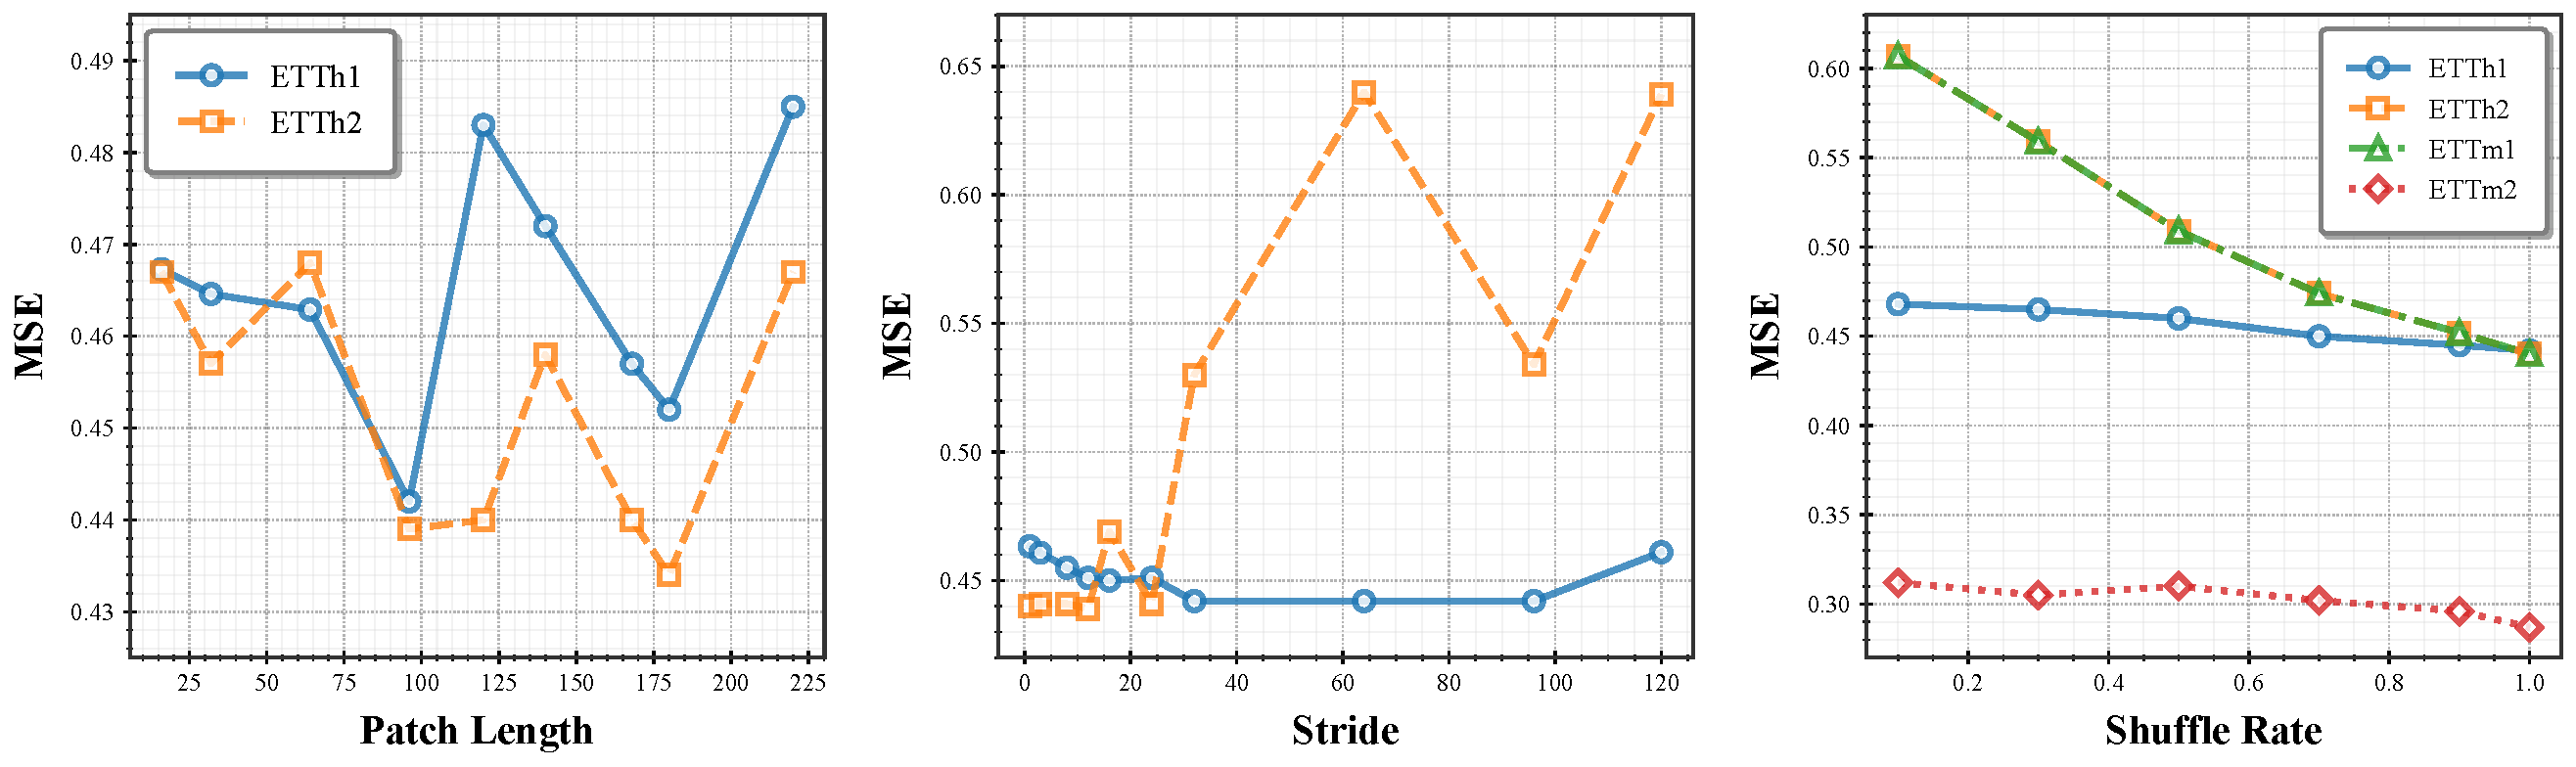
\includegraphics[page=1, width=1.0\textwidth, keepaspectratio]{./images/ablation_study_colorful.pdf}
\caption{Ablation study on the hyperparameter sensitivity of the TPS method. The y-axis shows the MSE averaged over five runs, while the x-axis represents the patch length, stride, or shuffle rate. Experiments were conducted using the LightTS model with a prediction length of 336 on the ETT datasets.}
    \label{fig:ablation_lightts}
\end{figure}


Following the evaluation protocol outlined in the paper~\cite{zhao2024dominantshufflesimplepowerful}, we conducted experiments using t-distributed stochastic neighbor embeddings (t-SNE) to compare the original data and the augmented data generated by each augmentation method on the ETTh2 dataset, utilizing the DLinear model with a prediction length of 336 (see Figure~\ref{fig:tsne}). We applied various augmentation techniques, including Upsample, FreqAdd, FreqPool, FreqMask, FreqMix, Dominant Shuffle, and our proposed method, TPS, with different parameter settings. The TPS parameters—denoted as (patch length, stride, shuffle rate)—were carefully tuned, and the configuration (32, 5, 1) yielded the best performance for the ETTh2 dataset. Our analysis suggests that ETTh2 does not require heavy noise injection, which aligns with the choice of smaller patch and stride values. TPS enables the generation of diverse augmented samples while preserving the core characteristics of the original signal, thereby showcasing the method's flexibility through parameter tuning. For instance, using a different configuration such as (120, 24, 1) introduces more noise due to larger patching, yet it still maintains the underlying signal structure, highlighting TPS's robustness across different augmentation intensities.



\begin{figure}[h!]
    \centering
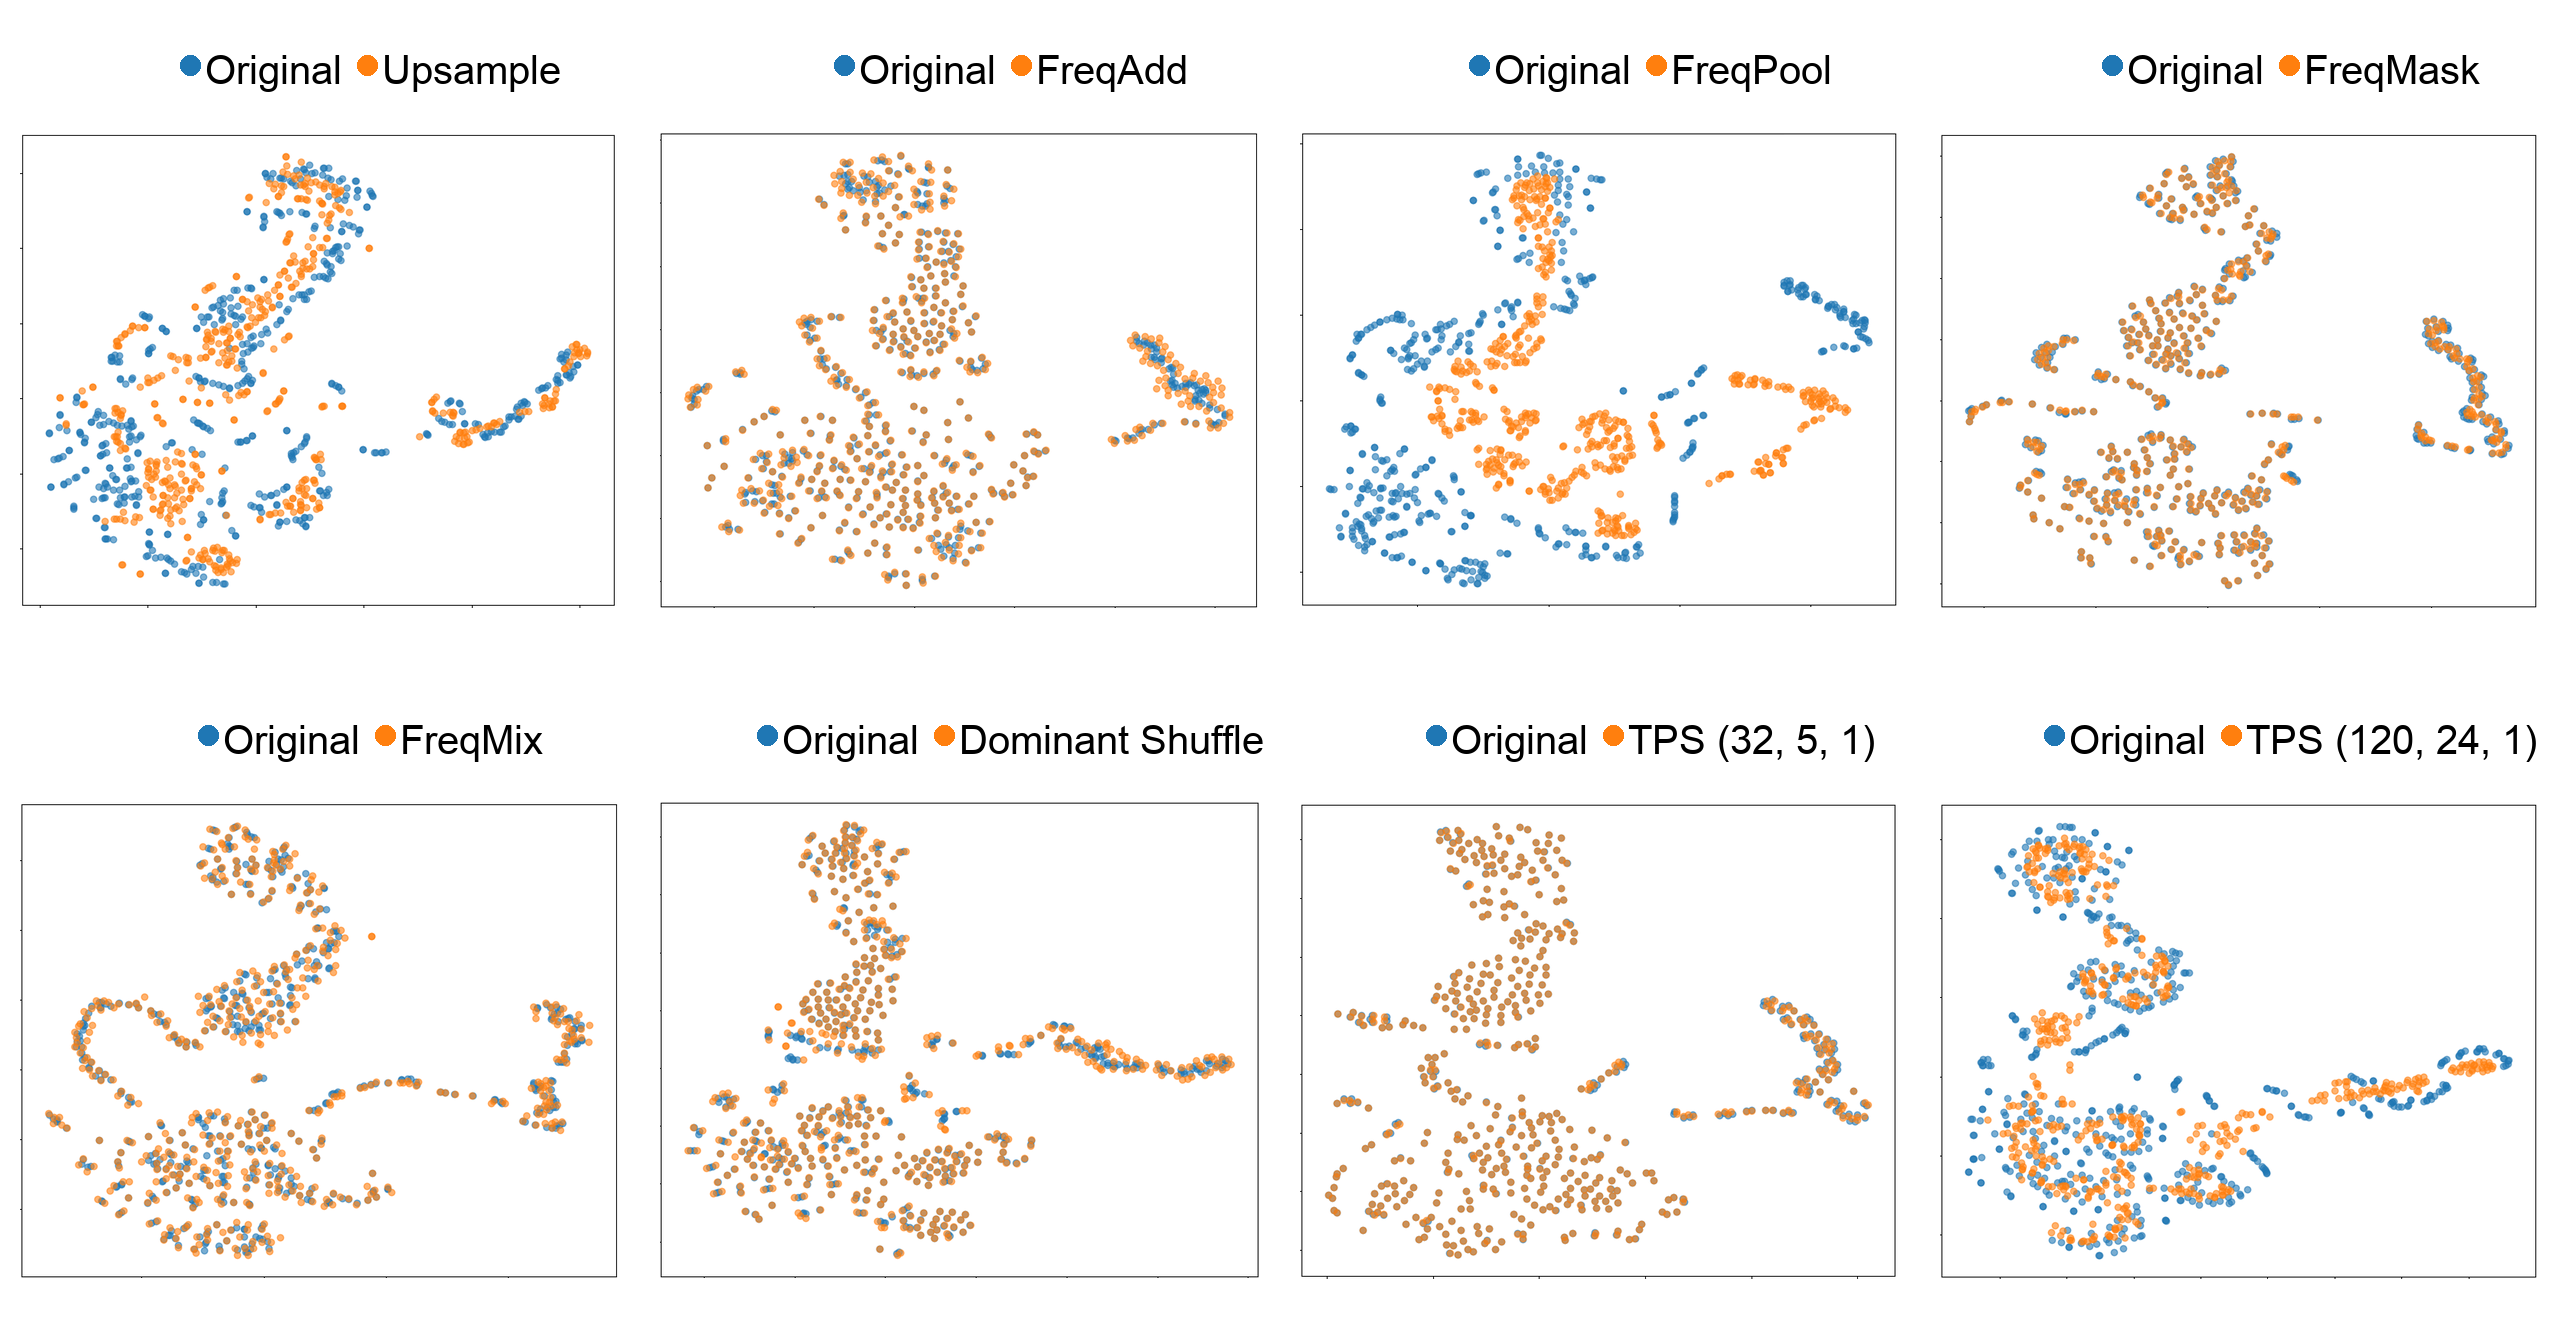
\includegraphics[page=1, width=1.0\textwidth, keepaspectratio]{./images/tsne_result.png}
\caption{t-SNE visualization of original and augmented data on the ETTh2 dataset using the DLinear model with a prediction length of 336.  A closer overlap between the original and augmented points indicates better distributional alignment and lower out-of-distribution issue. \textbf{Best viewed in color.}}
    \label{fig:tsne}
\end{figure}




To quantitatively assess the distributional similarity, we computed three metrics:
\begin{itemize}
    \item The \textbf{Kolmogorov–Smirnov (KS) statistic} measures the maximum difference between the cumulative distribution functions of two data, with higher values indicating greater distributional divergence~\cite{gchron-5-263-2023}.

    \item The \textbf{Wasserstein Distance}, which quantifies the minimum effort required to transform one distribution into another, is more robust to differences in shape than the KS statistic~\cite{gchron-5-263-2023, Iglesias2023}.
    
    \item The \textbf{Dynamic Time Warping (DTW)} distance, commonly used for time series, measures similarity between sequences~\cite{iwana2020timeseriesdataaugmentation, Iglesias2023}.


\end{itemize}

As shown in Table~\ref{tab:dist_metrics}, TPS (32, 5, 1) demonstrates superior performance across the most critical metrics, achieving the lowest Wasserstein distance (0.0097) and DTW distance (1.46), indicating exceptional preservation of both distributional geometry and temporal structure. While the KS statistic (0.0848) is moderate compared to Dominant Shuffle (0.0688), this suggests that TPS introduces controlled distributional variations without destroying fundamental data characteristics. The dramatically lower DTW distance for TPS compared to other methods (1.46 vs. 4.91-14.72) highlights its superior ability to maintain temporal dependencies, which are crucial for forecasting tasks. These results support our hypothesis that TPS generates realistic and semantically consistent augmentations with minimal distributional shift, successfully balancing the trade-off between introducing beneficial variations and preserving essential time series characteristics.

\begin{table}[h!]
\centering
\renewcommand{\arraystretch}{1.0}
\begin{adjustbox}{max width=\textwidth}
\begin{tabular}{lccc}
\toprule
\textbf{Method} & \textbf{Avg. KS Stat} $\downarrow$ & \textbf{Avg. Wasserstein} $\downarrow$ & \textbf{Avg. DTW} $\downarrow$ \\
\midrule
Upsample            & 0.0202 & 0.0177 & 8.73 \\
FreqAdd             & 0.1019 & 0.1475 & 8.55 \\
FreqPool            & 0.3366 & 0.3839 & 14.72 \\
FreqMask            & 0.0793 & 0.0523 & 4.91 \\
FreqMix             & 0.0756 & 0.0855 & 7.12 \\
Dominant Shuffle    & \textbf{0.0688} & 0.0550 & 6.02 \\
TPS (32, 5, 1)      & 0.0848 & \textbf{0.0097} & \textbf{1.46} \\
\bottomrule
\end{tabular}
\end{adjustbox}
\caption{Comparison of distribution shift metrics across various augmentation methods on the ETTh2 dataset using the DLinear model with a prediction length of 336. The metrics include the average Kolmogorov–Smirnov (KS) statistic, Wasserstein distance, and Dynamic Time Warping (DTW), where lower values indicate greater similarity to the original data.}
\label{tab:dist_metrics}
\end{table}


The ablation study in Figure~\ref{fig:augsizetsf} describes experiments conducted with varying augmentation sizes—1, 2, 3, 4, and 5—using the PatchTST model on the ETTh1 and ETTh2 datasets with a prediction length of 96. An augmentation size of 2 means that the augmented sample set is doubled by applying the augmentation method twice. This analysis helps to determine whether each method continues to improve performance as the augmentation size increases or whether it introduces excessive external noise.
The results show that FreqMix benefits from increased augmentation size on both datasets and FreqMask improves only on ETTh2 when applied twice. In contrast, other methods tend to degrade in performance as augmentation size increases. Notably, TPS on ETTh1 shows minimal performance variation even at an augmentation size of 4, suggesting that it introduces little external noise. This is not the case for methods like Upsample and FreqMask, which show greater sensitivity.
Dominant Shuffle and FreqMix exhibit stable performance across augmentation sizes and appear not to introduce significant noise. On the ETTh2 dataset, however, TPS shows signs of performance degradation at higher augmentation sizes, possibly due to suboptimal hyperparameter settings. Nonetheless, for other models and prediction lengths on ETTh2, TPS has shown to be generally stable across different augmentation sizes.


\begin{figure}[h!]
    \centering
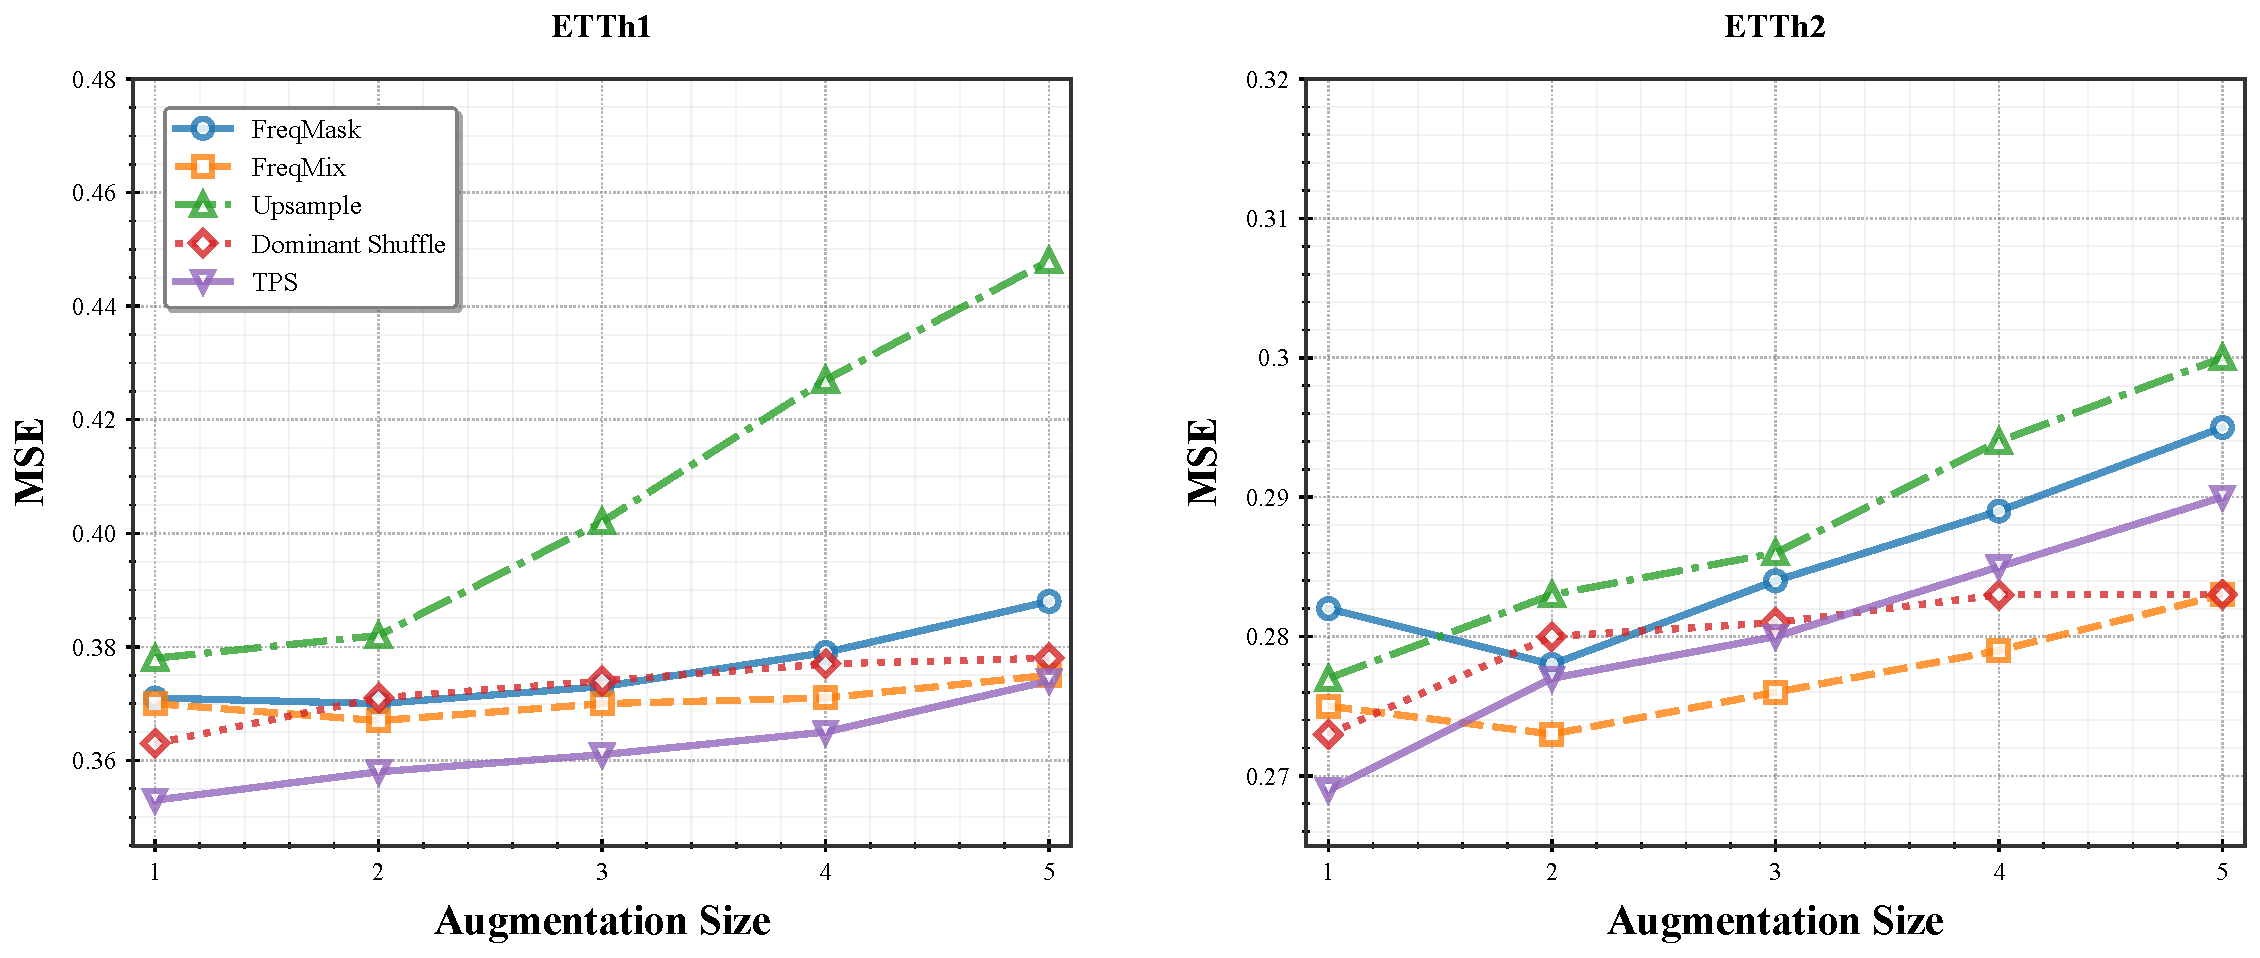
\includegraphics[page=1, width=1.0\textwidth, keepaspectratio]{./images/augmentation_size_analysis.pdf}
\caption{Impact of varying augmentation sizes (1–5) on forecasting performance using the PatchTST model with a prediction length of 96 on the ETTh1 and ETTh2 datasets. The results demonstrate how different augmentation methods respond to increasing augmentation intensity, highlighting stability or degradation in performance.}
    \label{fig:augsizetsf}
\end{figure}





We conducted experiments using different augmentation ratios — 0.1, 0.3, 0.5, 0.7, and 1.0 — with the PatchTST model on the ETTh1 and ETTh2 datasets, using a prediction length of 96 in the Figure~\ref{fig:augratio}. The augmentation methods evaluated include FreqMask, FreqMix, Upsample, Dominant Shuffle, and our proposed method, TPS. Here, the augmentation ratio refers to the proportion of augmented samples included in each training batch, meaning that lower ratios correspond to fewer augmented samples.

Our results show that TPS consistently achieves the lowest MSE across both datasets when using the full augmentation ratio (1.0). Remarkably, even with only 10\% (i.e., a ratio of 0.1) of augmented samples, TPS outperforms all other augmentation methods at their respective ratios.

\begin{figure}[h!]
    \centering
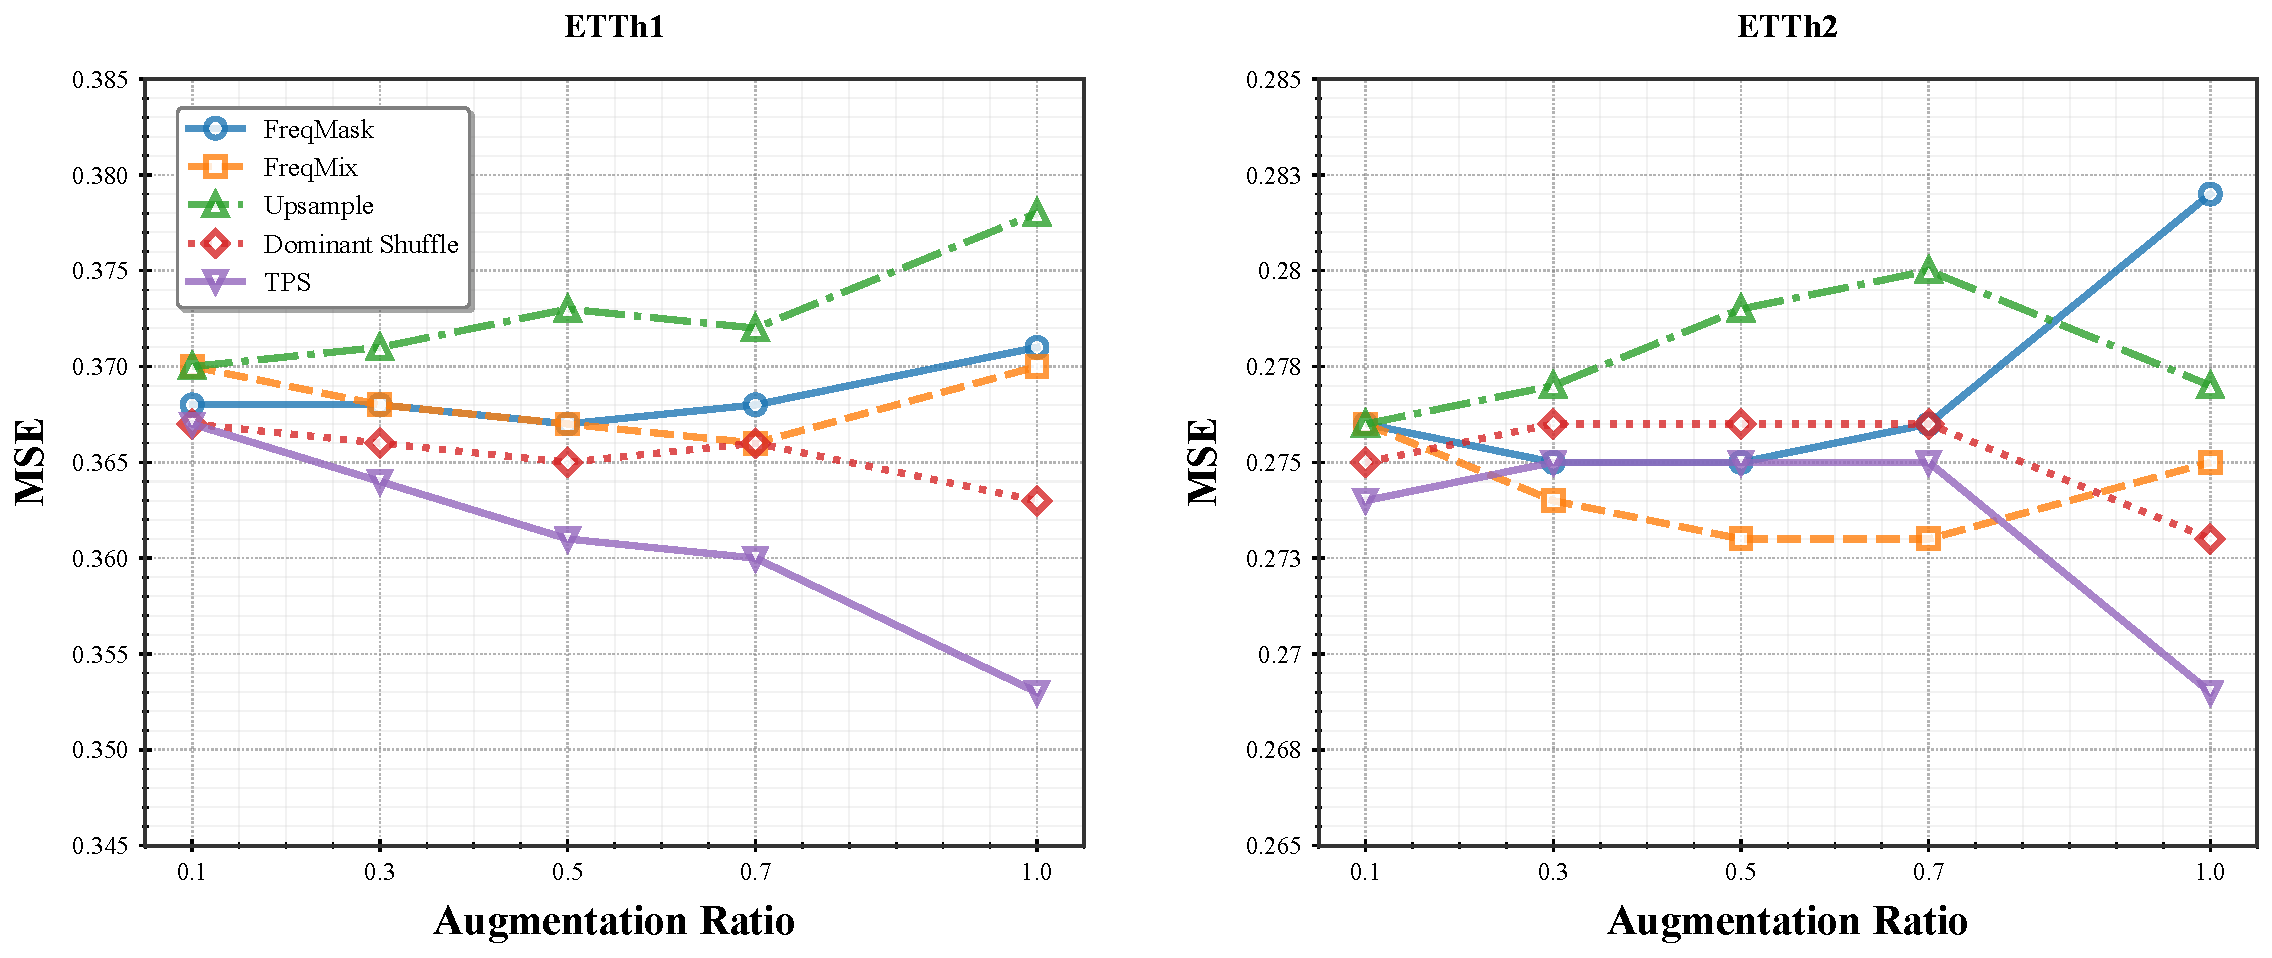
\includegraphics[page=1, width=1.0\textwidth, keepaspectratio]{./images/augmentation_ratio_analysis.pdf}
\caption{Effect of varying augmentation ratios (0.1 to 1.0) on the MSE performance of different augmentation methods using the PatchTST model with prediction length 96 on the ETTh1 and ETTh2 datasets. The augmentation ratio indicates the proportion of augmented samples used during training.}
    \label{fig:augratio}
\end{figure}



The final ablation study for time series forecasting evaluates the impact of different data augmentation methods on training time. Table~\ref{tab:augmentation_comparison} summarizes this comparison, conducted using the TSMixer model on the ETTh2 dataset with a prediction length of 720. The \textbf{Aug. Time} column reports the time required to apply the augmentation (in milliseconds), while the \textbf{Epoch Time} indicates the average training time per epoch (in seconds). The \textbf{Overhead} column shows the relative increase in epoch time (\%) compared to the baseline with no augmentation.

As shown in the table, TPS introduces a moderate augmentation time and only a modest increase in epoch time relative to the baseline. In contrast, Dominant Shuffle significantly increases the training cost, more than tripling the epoch time. Notably, for most augmentation methods (including TPS), the overhead remains well below twice the baseline training time. For Dominant Shuffle, we used the authors’ original implementation.


\begin{table}[h!]
\centering
\footnotesize
\vspace{0.2cm}
\renewcommand{\arraystretch}{1.1}
\begin{tabular}{lccc}
    \toprule
    \textbf{Method} & \textbf{Aug. Time (ms)} & \textbf{Epoch Time (s)} & \textbf{Overhead (\%)} \\
    \midrule
    None  & 0.000 & 2.298 & 0.00 \\
    \midrule
    FreqPool        & 1.023 & 2.611 & 13.63 \\
    FreqMask        & 1.097 & 2.633 & 14.59 \\
    FreqAdd         & 1.151 & 2.635 & 14.67 \\
    RobustTAD-m     & 1.603 & 2.690 & 17.08 \\
    FreqMix         & 1.573 & 2.720 & 18.36 \\
    RobustTAD-p     & 1.659 & 2.762 & 20.19 \\
    WaveMix         & 2.287 & 2.864 & 24.64 \\
    Upsample        & 2.486 & 2.944 & 28.14 \\
    WaveMask        & 3.809 & 3.145 & 36.86 \\
    \midrule
    TPS            & 7.688  & 4.094 & 78.15 \\
    Dominant Shuffle    & 22.908 & 7.698 & 235.02 \\
    \bottomrule
\end{tabular}
\vspace{0.2cm}
\caption{Comparison of data augmentation methods based on their impact on training time and computational overhead. Results are obtained using the TSMixer model on the ETTh2 dataset with a prediction length of 720. \textit{Aug. Time} refers to the time (in milliseconds) required to apply the augmentation, \textit{Epoch Time} represents the average training time per epoch (in seconds), and \textit{Overhead} indicates the percentage increase in epoch time relative to the baseline (None).}
\label{tab:augmentation_comparison}
\end{table}


\subsection{Ablation studies for Time Series Classification}  \label{subsec:ablation-tsc}

In these two ablation studies for time series classification, we used only MiniRocket for the univariate datasets and followed the same training pipeline throughout.

Figure~\ref{fig:augratiotsc} presents the ablation study on augmentation size for classification tasks, conducted on nine univariate time series datasets using the MiniRocket model. For each dataset, we selected the top five augmentation methods and compared them against our proposed method, TIPS, across augmentation sizes ranging from 1 to 5. For example, an augmentation size of 2 means each sample is augmented twice, effectively doubling the size of the augmented data.
From the figure, we observe that—except for the \textit{Car} and \textit{Meat} datasets—TIPS consistently maintains its superior performance across all augmentation sizes of the top five competing methods. In the \textit{Beef} dataset, TIPS improves from third place to second when using two augmentations. Overall, our method achieves its peak accuracy with one or sometimes two augmentation sizes. Beyond this point, additional augmentation does not lead to further improvements, indicating that TIPS is highly effective with minimal augmentation size. In contrast, some other methods often require four augmented samples to reach their maximum performance.


\begin{figure}[h!]
    \centering
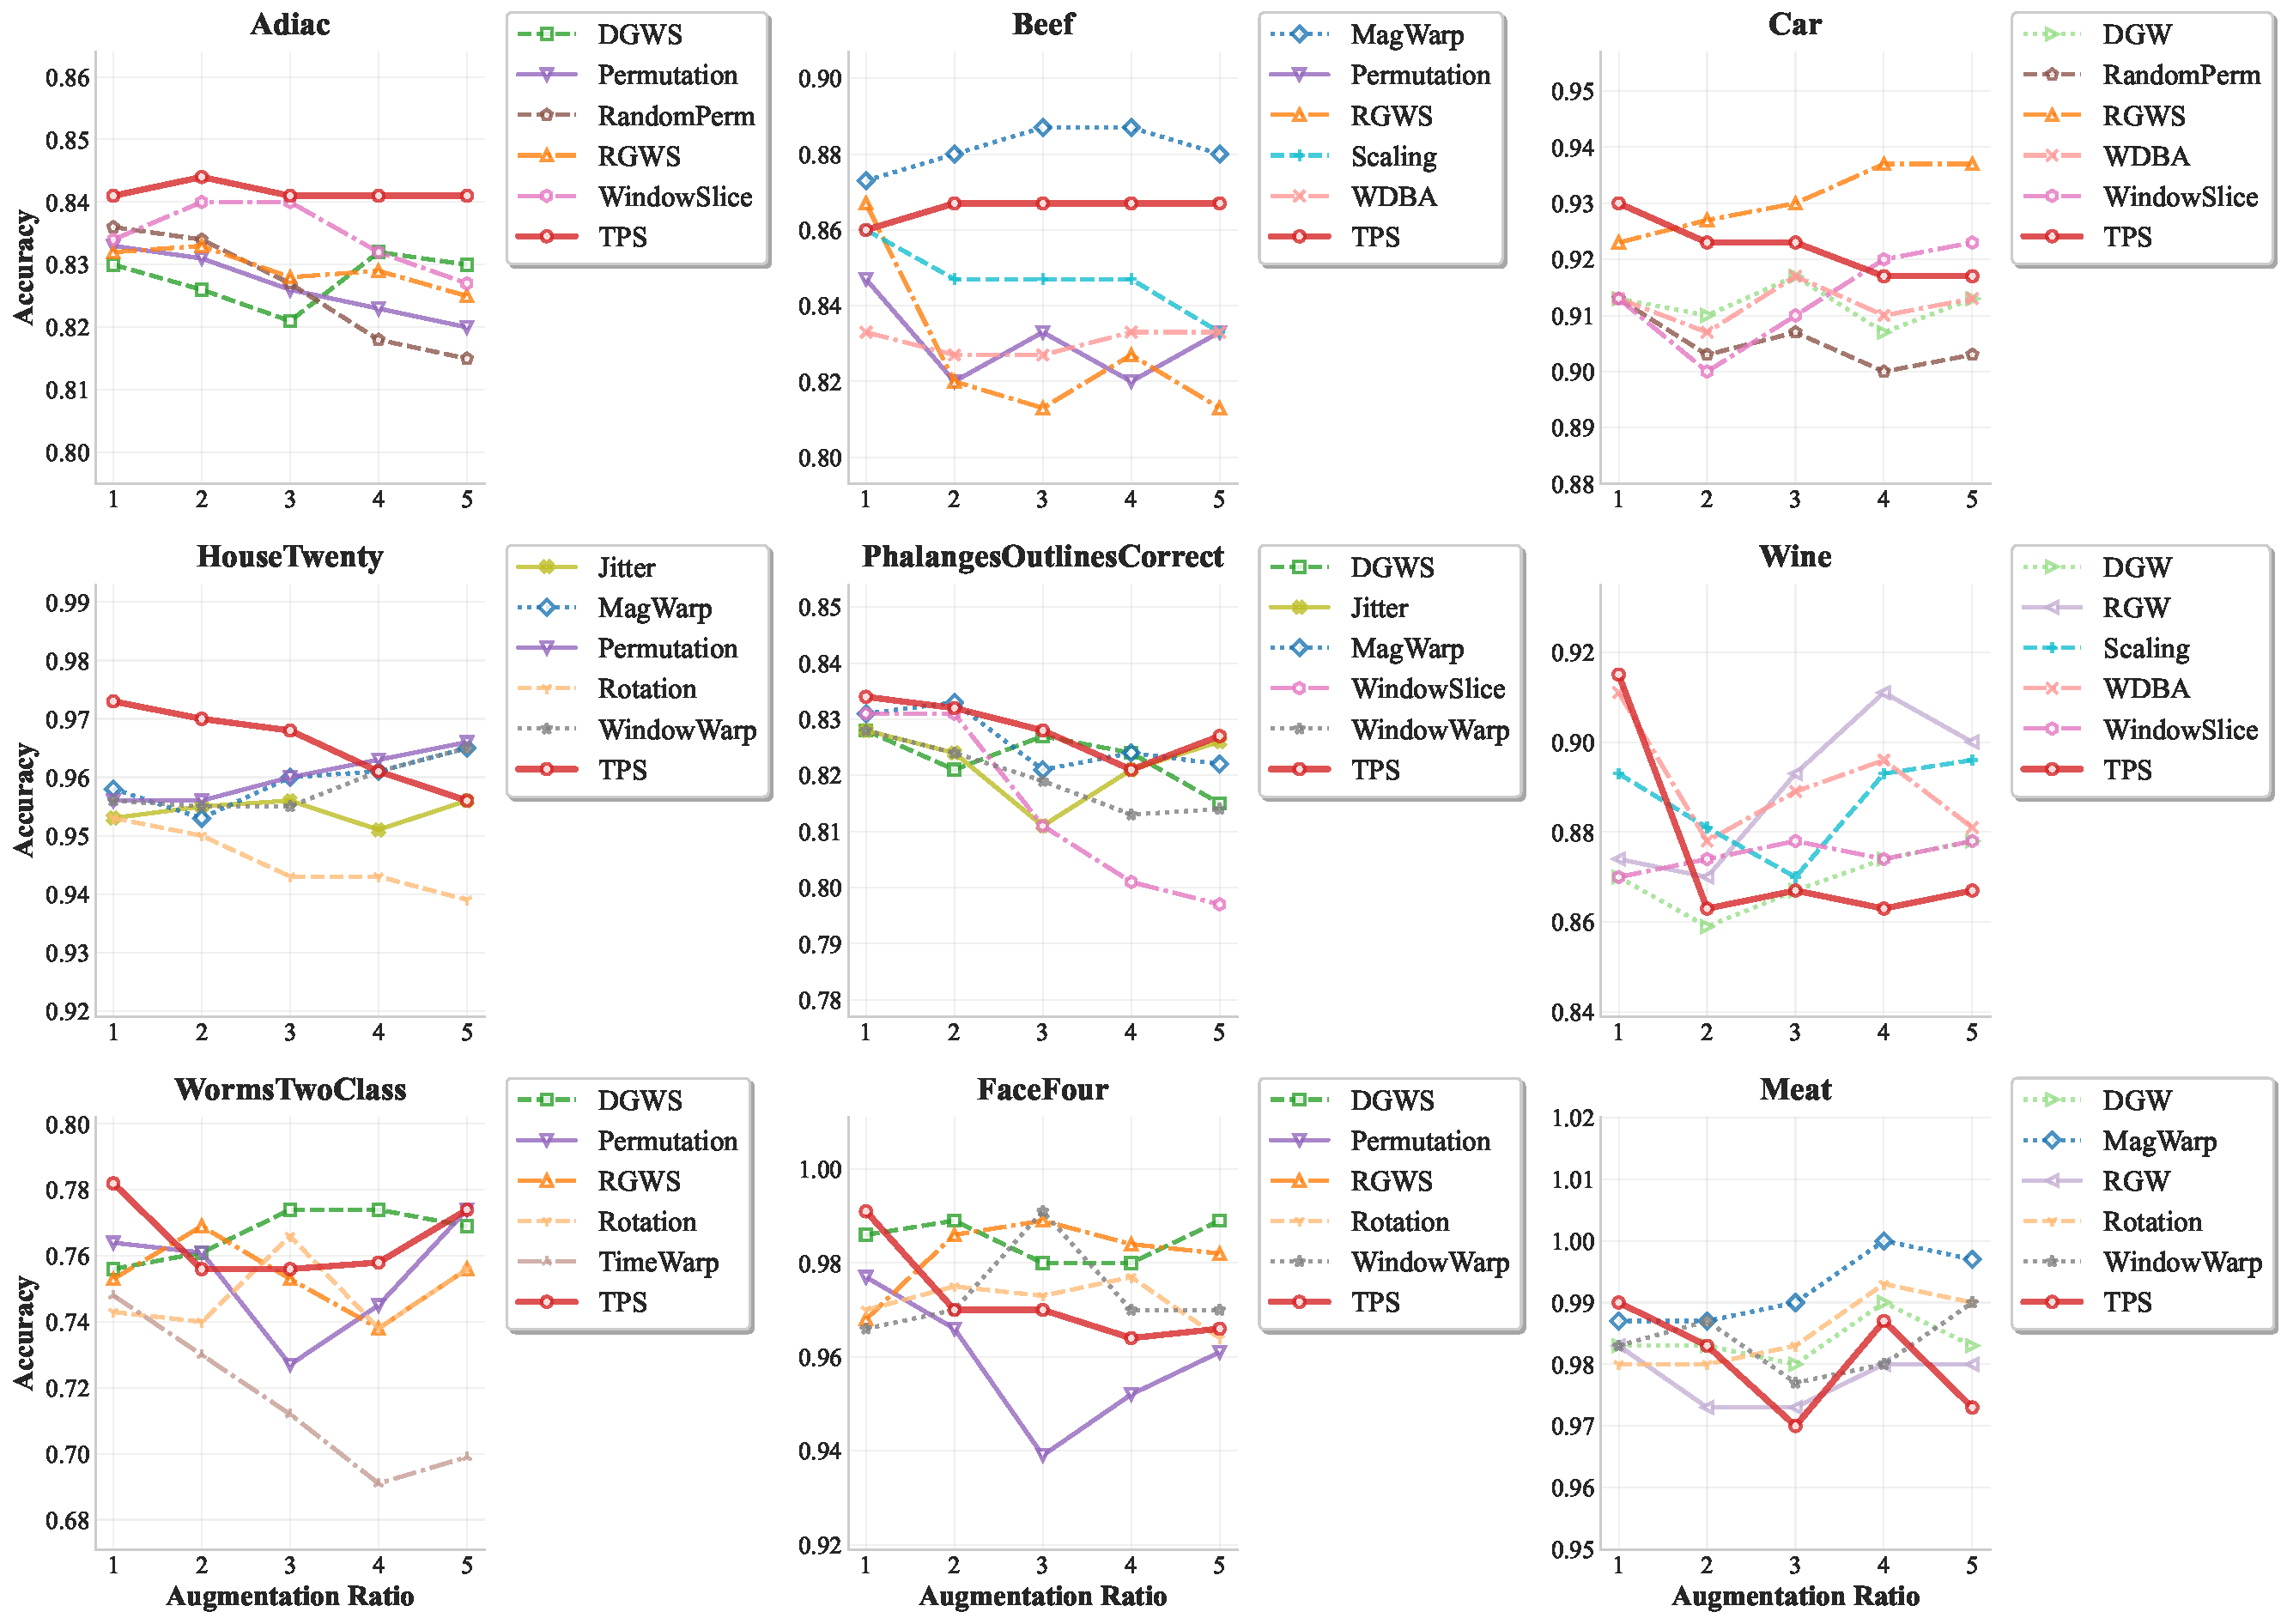
\includegraphics[page=1, width=1.0\textwidth, keepaspectratio]{./images/improved_tsc_results.pdf}
\caption{Ablation study on augmentation size for classification tasks across 9 univariate time series datasets using MiniRocket. For each dataset, the top five augmentation methods are compared against our proposed method TIPS. Augmentation sizes from 1 to 5 are evaluated.}
    \label{fig:augratiotsc}
\end{figure}




The final ablation study for classification tasks examines the runtime of each augmentation method. Table~\ref{tab:aug_times_tsc} reports the time required to execute each method, measured in seconds under the MiniRocket model on the HandOutlines dataset. The \textbf{Aug. Time} column indicates the time taken by each augmentation.
We observe that TIPS has a moderate runtime compared to other fast augmentations, such as Magnitude Warping and Time Warping; however, it is significantly more efficient than computationally intensive methods like RGW and DGW. This highlights that our method achieves superior classification performance with substantially lower computational cost than the most complex augmentation strategies.

\begin{table}[h!]
\centering
\begin{tabular}{lr}
\toprule
\textbf{Method} & \textbf{Aug. Time (s)} \\
\midrule
 Jitter         & 0.14 \\
 Scaling        & 0.04 \\
 Rotation       & 0.04 \\
 Permutation    & 0.08 \\
 RandPermutation   & 0.13 \\
 Mag. Warping        & 0.45 \\
 Time Warping       & 0.52 \\
 Window Slice    & 0.12 \\
 Window Warping     & 0.17 \\
 TIPS           & 49.76 \\
SPAWNER        & 1,612.38 \\
RGW            & 1,761.13 \\
RGWs           & 15,334.64 \\
 DGW            & 26,287.65 \\
 wDBA           & 59,832.97 \\
 DGWs           & 247,505.86 \\
\bottomrule
\end{tabular}
\caption{Runtime (in seconds) for various time series augmentation methods on the HandOutlines dataset using the MiniRocket model. The results reflect the computational cost required to apply each augmentation.}

\label{tab:aug_times_tsc}
\end{table}








% %%%%%%%%%%%%%%%%%%%%%%%%%%%%%%%%%%%%%%%%%
 %!TEX root = ../Master_template.tex
\chapter{Conclusion} \label{chapter:conclusion}



This master’s thesis addresses a critical gap in augmentation strategies by proposing methods that are effective for both time series forecasting and classification. Drawing inspiration from data augmentation techniques in computer vision—such as PatchShuffle and PatchMix—this study introduces a novel approach based on creating overlapping segments termed temporal patches, which are then shuffled using a simple but effective strategy.

The first proposed method, \textbf{Temporal Patch Shuffle (TPS)}, is designed for both forecasting and classification. For classification tasks, we further extend TPS by leveraging class labels: instead of shuffling patches within the same sample, we replace selected patches with those from other samples of the same class. This enhanced variant is known as the \textbf{Temporal Index Patch Shuffle (TIPS)}. Both TPS and TIPS consistently achieve strong performance across a wide range of models and datasets.

In forecasting, TPS demonstrated notable improvements over existing methods. Specifically, TPS achieved average MSE improvements of \textbf{2.98\%}, \textbf{5.83\%}, \textbf{3.16\%}, \textbf{2.26\%}, and \textbf{10.90\%} over the second-best augmentation method when applied to TSMixer, DLinear, PatchTST, TiDE, and LightTS models, respectively. Out of 28 total experiments ($4$ prediction lengths $\times$ $7$ datasets), TPS ranked first in over 20 settings—demonstrating its robustness across architectures and settings.
In classification, TPS also outperformed all other augmentation methods on both univariate and multivariate datasets using the MiniRocket and MultiRocket models. TIPS further improved upon TPS itself. On average, TPS and TIPS achieved \textbf{1.87\%} and \textbf{3.30\%} improvement over the second-best method (excluding TPS and TIPS) in univariate and multivariate classification, respectively. Among 30 datasets, TPS and TIPS ranked in the Top-2 on \textbf{80\%} of them and achieved the Top-1 position on \textbf{70\%} of the multivariate datasets (10 in total).

Beyond achieving superior performance over existing augmentation methods, both methods contribute to improved generalization and robustness. Standard deviations across multiple runs are consistently low, indicating stable performance. Extensive ablation studies further support our design choices, including: component-wise analysis of TPS, sensitivity to hyperparameters, evaluation of out-of-distribution (OOD) issues and external noise, augmentation size and ratio effects, and computational overhead. These studies collectively reinforce the methodological rationale behind our design. Importantly, both TPS and TIPS are lightweight, scalable, and easily integrable into a wide variety of model architectures.
We also re-implemented many augmentation methods from prior work, especially those without publicly available code, to ensure a fair and comprehensive comparison. For classification tasks, most implementations were publicly available. Our evaluation protocol corrects flaws from previous studies and, within computational constraints, ensures a fair comparison under consistent settings.

In summary, this thesis not only introduces two novel augmentation methods—TPS and TIPS—that achieve superior performance but also presents a thorough re-evaluation of existing methods using modern architectures for both time series forecasting and classification.
Both of these methods can be applied effectively to broader contexts in time series analysis and easily adapted with minimal changes. The following sections will address the limitations and challenges of our approach and outline potential directions for future research.


\section{Challanges \& Limitations} \label{sec:limitations}

Our study faced several challenges primarily due to computational constraints, as we relied on a combination of university cluster access and self-funded Amazon AWS instances. These limitations prevented us from conducting an extensive hyperparameter search across all models and significantly constrained the number of configurations we could explore for TPS. As discussed in Chapter~\ref{chapter:experiments}, we performed a thorough hyperparameter search for the TSMixer model, one of the best-performing architectures, across most augmentation methods, which consumed substantial time and resources. However, for other augmentation methods, we had to use the hyperparameters reported in the original papers. This introduces a potential issue: some of those parameters have been selected based on test loss rather than validation loss, which could affect the fairness and reproducibility of comparisons.

Additionally, due to time and resource constraints, we were unable to run models for the full number of epochs used in the original studies (e.g., 1000 epochs). Instead, we limited training to 20 epochs and adopted appropriate learning rate schedules to mitigate the impact. This compromise kept performance degradation minimal but could be improved with access to more powerful and numerous GPU instances.



We did not train models with augmentations on the Electricity Consumption Load (ECL), Traffic, and Solar-Energy datasets~\cite{lai2018modelinglongshorttermtemporal} for time series forecasting due to high computational demands; however, this work can be extended to these datasets with access to additional GPU resources. For time series classification, we implemented only models from the ROCKET family~\cite{Dempster_2020}—specifically MiniRocket~\cite{Dempster_2021} and MultiRocket~\cite{tan2022multirocketmultiplepoolingoperators}. Although these models are state-of-the-art in terms of efficiency and accuracy, evaluating TPS and TIPS on other architectures, such as InceptionTime, would help assess generalization and ensure fairness across different model types. We could also reimplement the Stratified Fourier Coefficients Combination (SFCC)~\cite{sfccYang2023} method to evaluate its effectiveness compared to other augmentation techniques. Unfortunately, due to time constraints, we were unable to reproduce it based on the original paper's description. However, as shown in Table~\ref{tab:augmentation_performance}, SFCC ranks fifth—below RGWs, DGWs, Window Warping, and Random Permutation—all of which were already included in our evaluation.

These resource constraints also limited the breadth of our ablation studies. For classification tasks, we conducted only two ablations; further analysis would have provided more profound insight. In the forecasting context, most of our ablation studies focused on the ETTh1 and ETTh2 datasets. Ideally, this should be extended to include ETTm1 and ETTm2 datasets for a more comprehensive evaluation.

We will elaborate on some of these points and propose additional directions for future research in the next section.

\section{Future Work} \label{sec:future}


We have applied our proposed augmentation methods to various forecasting models, including linear models, MLP-based architectures, and Transformer-based models. A natural next step would be to evaluate the effectiveness of our method on other types of models, such as Graph Neural Networks (GNNs) and Recurrent Neural Networks (RNNs). For example, it would be valuable to investigate how TPS performs when integrated into models like FourierGNN~\cite{yi2023fouriergnnrethinkingmultivariatetime} and other GNN-based approaches~\cite{NEURIPS2020_ce1aad92, cao2021spectraltemporalgraphneural}.
In addition to the PatchTST model evaluated in our experiments, other Transformer-based models could also benefit from our method. Another model for implementation can be CycleNet~\cite{lin2024cyclenetenhancingtimeseries}, a recently proposed state-of-the-art model for time series forecasting.  We applied a subset of the most impactful augmentation methods—selected based on their performance in Chapter~\ref{chapter:experiments}—to the CycleNet model. We also performed extensive hyperparameter tuning specifically for the ETTh1 dataset.
Table~\ref{tab:cycle_etth1} reports the results using Mean Squared Error (MSE) for prediction lengths of \{96, 192, 336, 720\}, with the final column showing the average performance. In this
table, RobustTAD-m/p refers to the best result selected from RobustTAD
implementations applied to either the magnitude or phase components. Freq-MixMax denotes the best outcome obtained between FreqMax and FreqMix. TPS achieved a \textbf{1.74\%} improvement over the second-best method, Dominant Shuffle. The dagger ($\dagger$) symbol indicates that the parameters of augmentation methods are tuned extensively, while \textbf{None*} refers to the original results reported in the CycleNet paper. Our reimplementation outperformed the original baseline, which we attribute to a more effective learning rate scheduler for the ETTh1 dataset.
Lastly, a very recent model called TQ-Net~\cite{lin2025temporalquerynetworkefficient}, which builds upon and improves CycleNet, could be another strong candidate for experimenting with our proposed augmentation methods.




\begin{table}[h!]
\centering
\renewcommand{\arraystretch}{1.3}
\begin{adjustbox}{max width=\textwidth}
\begin{tabular}{l|c|c|c|c||c}
\toprule
\textbf{Method} & \textbf{96} & \textbf{192} & \textbf{336} & \textbf{720} & \textbf{AVG} \\
\midrule
None*              & 0.378 ± 0.0010 & 0.426 ± 0.0010 & 0.464 ± 0.0010 & 0.461 ± 0.0010 & 0.432 ± 0.0010 \\
None               & 0.368 ± 0.0022 & 0.407 ± 0.0038 & 0.406 ± 0.0030 & 0.446 ± 0.0027 & 0.407 ± 0.0026 \\
RobustTAD-m/p    & 0.368 ± 0.0026 & 0.403 ± 0.0031 & 0.400 ± 0.0011 & 0.444 ± 0.0025 & 0.404 ± 0.0020 \\
FreqAdd$^\dagger$  & 0.368 ± 0.0050 & 0.406 ± 0.0049 & 0.400 ± 0.0025 & 0.441 ± 0.0066 & 0.404 ± 0.0040 \\
FreqPool$^\dagger$ & 0.402 ± 0.0012 & 0.413 ± 0.0021 & 0.408 ± 0.0005 & 0.447 ± 0.0024 & 0.418 ± 0.0009 \\
Upsample$^\dagger$ & 0.377 ± 0.0007 & 0.412 ± 0.0030 & 0.402 ± 0.0021 & \cellcolor{secondcolor} 0.437 ± 0.0038 & 0.407 ± 0.0016 \\
Freq-MixMask$^\dagger$ & \cellcolor{secondcolor}0.366 ± 0.0008 & 0.404 ± 0.0043 & 0.404 ± 0.0009 & 0.448 ± 0.0024 & 0.406 ± 0.0009 \\
Dominant Shuffle$^\dagger$  & \cellcolor{bestcolor} \textbf{0.364 ± 0.0031} & \cellcolor{secondcolor} 0.401 ± 0.0012 & \cellcolor{secondcolor} 0.400 ± 0.0022 & 0.441 ± 0.0016 & \cellcolor{secondcolor} 0.402 ± 0.0027 \\
TPS$^\dagger$           & 0.368 ± 0.0006 & \cellcolor{bestcolor} \textbf{0.399 ± 0.0029} & \cellcolor{bestcolor} \textbf{0.387 ± 0.0041} & \cellcolor{bestcolor} \textbf{0.424 ± 0.0019} & \cellcolor{bestcolor} \textbf{0.395 ± 0.0029} \\
\cmidrule(lr){1-6}
\textbf{Improvement} & \cellcolor{worstcolor} --1.10\% & \cellcolor{bestcolor} \textbf{0.50\%} & \cellcolor{bestcolor} \textbf{3.25\%} &  \cellcolor{bestcolor} \textbf{2.97\%} & \cellcolor{bestcolor} \textbf{1.74\%} \\
\bottomrule
\end{tabular}
\end{adjustbox}
\caption{Forecasting performance (MSE ± std) of CycleNet on the ETTh1 dataset using prediction lengths \{96, 192, 336, 720\}. $\dagger$ indicates that the method was extensively tuned. None* refers to the original results reported in the CycleNet paper, while None is our reimplementation using a different learning rate scheduler.}
\label{tab:cycle_etth1}
\end{table}

We have implemented the augmentation methods exclusively for multivariate time series forecasting; however, they can be extended to univariate settings as well. For example, the study by Chen et al.~\cite{chen2023fraugfrequencydomainaugmentation} explored \textbf{cold-start forecasting}, where only 10\% or 20\% of the training data is used to assess how augmentation impacts performance. This scenario presents an important and practical area for further investigation using our proposed methods.
For time series classification, we have utilized only MiniRocket and MultiRocket from the ROCKET family~\cite{Dempster_2020}. It would be valuable to extend the evaluation to other popular models such as InceptionTime~\cite{Ismail_Fawaz_2020}, which is widely regarded as a strong baseline in classification benchmarks. Moreover, our experiments were limited to 30 of the 128 univariate datasets and 10 of the 30 multivariate datasets. A thorough assessment of all UCR and UEA datasets would provide a more complete performance ranking and improve the generalizability of our results.


There are several promising directions for extending or modifying the TPS and TIPS frameworks. One such extension involves \textbf{adaptive patch sizing}, where the patch length and stride are not predetermined but are dynamically adjusted according to the statistical characteristics of the input sequence. This would allow the model to more precisely capture the diverse temporal patterns and structures across datasets or within a singular time series. Additionally, the \textbf{importance score} used to select patches for shuffling could be refined. Currently, we utilize patch-wise variance as an indicator of informativeness, positing that low-variance patches are less critical and more suitable for transformation. However, alternative strategies could provide better assessments of patch relevance. Investigating these alternatives in ablation studies may provide a deeper understanding of their effects on model generalization and robustness.


Our proposed augmentations can be applied to various tasks in time series analysis with minimal changes. For example, it would be interesting to investigate how these methods could enhance performance in self-supervised models that use contrastive learning, such as TS2Vec~\cite{Yue_Wang_Duan_Yang_Huang_Tong_Xu_2022} and TF-C~\cite{zhang2022selfsupervisedcontrastivepretrainingtime}. These augmentations could also be explored in combination with recent advancements, such as Dynamic Bad Pair Mining (DBPM)~\cite{lan2024enhancingtimeseriescontrastive}, which further refine contrastive learning frameworks. Importantly, the parameters of our proposed methods are flexible—allowing for less aggressive shuffling or the substitution of alternative transformation operations to suit specific use cases. Additionally, our approach can be integrated with other augmentation strategies, especially in the models mentioned above. In this sense, we believe that our methods are versatile, lightweight, and easy-to-integrate tools for a wide range of applications in time series analysis.



%%%%%%%%%%%%%%%%%%%%%%%%%%%%%%%%%%%%%%%%%
% ===========================
% Appendix Section Starts Here
% ===========================

% Again, content here or from external file
% \include{./chapters/appendix_code}

\clearpage
\addcontentsline{toc}{chapter}{Bibliography}
\bibliography{chapters/bibliography}

\bibliographystyle{apalike}


\clearpage
\appendix

% Switch to Roman numeral page numbering for appendices
\pagenumbering{roman}

% Fix Issue 1: Make "Appendices" link work correctly
% Add a phantom section that creates the proper anchor
\phantomsection
\addcontentsline{toc}{chapter}{Appendices}

% Reset chapter counter and use letters
\setcounter{chapter}{0}
\renewcommand{\thechapter}{\Alph{chapter}}

% Fix table/figure numbering to include appendix letter
\renewcommand{\thetable}{\thechapter.\arabic{table}}
\renewcommand{\thefigure}{\thechapter.\arabic{figure}}
\renewcommand{\theequation}{\thechapter.\arabic{equation}}



\chapter*{Appendix A: Pseudocode for FreqMask \& FreqMix} 
\setcounter{chapter}{1} % A = 1
% Reset counters for this appendix
\setcounter{table}{0}
\setcounter{figure}{0}
\setcounter{equation}{0}
\renewcommand{\thechapter}{A}
\refstepcounter{chapter}
\label{app:freqmask}


The pseudocodes for Frequency Masking (FreqMask) and Frequency Mixing (FreqMix) are presented in Algorithms~\ref{alg: freqmasking} and~\ref{alg: freqmixing}, respectively. As input, the methods take a look-back window and a target horizon, which are concatenated before applying the fast Fourier transform (FFT) (Lines~\ref{alg: freqmasking:concat}–\ref{alg: freqmasking:rfft}). A random mask is then created based on the shape of the frequency representation and the specified mask rate (Line~\ref{alg: freqmasking:mask}). This mask is applied to the frequency components, and the signal is reconstructed using the inverse FFT (Lines~\ref{alg: freqmasking:applymask}–\ref{alg: freqmasking:ifft}). The final augmented look-back window and target horizon are obtained by splitting the reconstructed signal (Line~\ref{alg: freqmasking:split}).

We use the original implementation by the authors, which includes an additional step to exclude dominant frequency components from masking~\cite{chen2023fraugfrequencydomainaugmentation}.

\begin{algorithm}
     \caption{Frequency Masking (FreqMask)~\cite{chen2023fraugfrequencydomainaugmentation}}
     \label{alg: freqmasking}
     \begin{algorithmic}[1]
         \REQUIRE
             Look-back window $x$, target horizon $y$, mask rate $\mu$
         \ENSURE
             Augmented look-back window $\tilde{x}$, augmented target horizon $\tilde{y}$
         \STATE $s = x \,\|\, y$ \COMMENT{Concatenate $x$ and $y$} \label{alg: freqmasking:concat}
         \STATE $S = \texttt{rFFT}(s)$ \COMMENT{Apply FFT to obtain frequency representation $S$} \label{alg: freqmasking:rfft}
         \STATE $m = \texttt{CreateRandomMask}(\texttt{len}(S), \mu)$ \COMMENT{Create random mask with mask rate $\mu$} \label{alg: freqmasking:mask}
         \STATE $\tilde{S} = \texttt{Masking}(S, m)$ \label{alg: freqmasking:applymask}
         \STATE $\tilde{s} = \texttt{irFFT}(\tilde{S})$ \label{alg: freqmasking:ifft}
         \STATE $\tilde{x}, \tilde{y} = \tilde{s}[0{:}b], \tilde{s}[b{:}b{+}t]$ \COMMENT{Split into augmented look-back and target} \label{alg: freqmasking:split}
     \end{algorithmic}
\end{algorithm}

The pseudocode for Frequency Mixing (FreqMix) is shown in Algorithm~\ref{alg: freqmixing}. This method uses two different training samples—each with its own look-back window and target horizon—typically obtained by randomly permuting batches. Like FreqMask, it applies transformations in the frequency domain, but with a key difference: it creates a random binary mask for one sample and uses its bitwise complement for the other (Lines~\ref{alg: freqmixing:mask1}–\ref{alg: freqmixing:mask2}). These masks are applied to the frequency components of the two samples, which are then summed (Line~\ref{alg: freqmixing:applymask}). The inverse FFT is used to reconstruct the signal, which is finally split into the augmented look-back window and target horizon (Lines~\ref{alg: freqmixing:ifft}–\ref{alg: freqmixing:split}).


\begin{algorithm}
   \caption{Frequency Mixing (FreqMix)~\cite{chen2023fraugfrequencydomainaugmentation}}
   \label{alg: freqmixing}
   \begin{algorithmic}[1]
       \REQUIRE
           Look-back windows $x_1$, $x_2$, target horizons $y_1$, $y_2$, mix rate $\mu$
       \ENSURE
           Augmented look-back window $\tilde{x}$, augmented target horizon $\tilde{y}$
       \STATE $s_1 = x_1 \,\|\, y_1$, \quad $s_2 = x_2 \,\|\, y_2$ \COMMENT{Concatenate input and target} \label{alg: freqmixing:concat}
       \STATE $S_1 = \texttt{rFFT}(s_1)$, \quad $S_2 = \texttt{rFFT}(s_2)$ \COMMENT{Compute frequency representations} \label{alg: freqmixing:rfft}
       \STATE $m_1 = \texttt{CreateRandomMask}(\texttt{len}(S_1), \mu)$ \COMMENT{Create binary mask for sample 1} \label{alg: freqmixing:mask1}
       \STATE $m_2 = \texttt{BitwiseNOT}(m_1)$ \COMMENT{Create inverted mask for sample 2} \label{alg: freqmixing:mask2}
       \STATE $\tilde{S} = \texttt{Masking}(S_1, m_1) + \texttt{Masking}(S_2, m_2)$ \COMMENT{Combine masked frequency components} \label{alg: freqmixing:applymask}
       \STATE $\tilde{s} = \texttt{irFFT}(\tilde{S})$ \COMMENT{Reconstruct signal via inverse FFT} \label{alg: freqmixing:ifft}
       \STATE $\tilde{x}, \tilde{y} = \tilde{s}[0{:}b], \tilde{s}[b{:}b{+}t]$ \COMMENT{Split into augmented look-back and target} \label{alg: freqmixing:split}
   \end{algorithmic}
\end{algorithm}





\chapter*{Appendix B: Ranking of Existing Augmentations for TSC}
\setcounter{chapter}{2} % B = 2
% Reset counters for this appendix
\setcounter{table}{0}
\setcounter{figure}{0}
\setcounter{equation}{0}
\renewcommand{\thechapter}{B}
\refstepcounter{chapter}
\label{app:tscranking}

The study by~\cite{gao2024dataaugmentationtimeseriesclassification} conducted comprehensive experiments across multiple time series classification datasets to evaluate and rank various data augmentation methods. The results, presented in Table~\ref{tab:augmentation-ranking}, reveal that conditional generative adversarial networks (cGANs) consistently underperform compared to the baseline (no augmentation), placing last or near last in the most datasets. This finding, along with the high computational cost associated with GAN-based methods, justifies the exclusion of both cGAN and TimeGAN from our evaluation benchmarks. The results also highlight that traditional methods, such as time warping (TW), window warping (WW), and permutation (PRM), generally achieve better average ranks, which are included in our evaluation.


\begin{table}[h!]
\centering
\renewcommand{\arraystretch}{1.3}
\begin{adjustbox}{max width=\textwidth}
\begin{tabular}{lcccccccccccccc}
\toprule
\textbf{Dataset} & \textbf{Jitter} & \textbf{Rotation} & \textbf{Scaling} & \textbf{MW} & \textbf{Slicing} & \textbf{TW} & \textbf{WW} & \textbf{PRM} & \textbf{RGW} & \textbf{DGW} & \textbf{SPAWNER} & \textbf{cGAN} & \textbf{Baseline} \\
\midrule
OPPORTUNITY     & 7 & 8  & 5  & 10 & 6  & 1 & 2 & 9 & 3 & 4  & 11 & 13 & 12 \\
HAR             & 5 & 6  & 4  & 9  & 8  & 1 & 7 & 2 & 10 & 3  & 11 & 12 & 13 \\
DEAP (Arousal)  & 9 & 12 & 10 & 8  & 2  & 1 & 4 & 3 & 6 & 5  & 13 & 11 & 7  \\
DEAP (Valence)  & 10 & 9 & 11 & 8  & 4  & 1 & 3 & 2 & 7 & 6  & 13 & 12 & 5  \\
BVDB            & 6 & 13 & 7  & 11 & 8  & 3 & 1 & 2 & 4 & 12 & 5  & 9  & 10 \\
PMDB            & 3 & 13 & 4  & 5  & 10 & 7 & 1 & 2 & 9 & 8  & 6  & 11 & 12 \\
\midrule
\textbf{Average Rank} & 6.67 & 10.17 & 6.83 & 8.50 & 6.33 & 2.33 & 3.00 & 3.33 & 6.50 & 6.33 & 9.83 & 11.33 & 9.83 \\
\bottomrule
\end{tabular}
\end{adjustbox}
\caption{Average ranking of data augmentation methods across six time series classification datasets. A lower rank indicates better performance. Methods like Time Warping (TW), Window Warping (WW), and Permutation (PRM) rank higher overall, while cGAN consistently underperforms compared to the baseline~\cite{gao2024dataaugmentationtimeseriesclassification}.}
\label{tab:augmentation-ranking}
\end{table}




\end{document}






\clearpage
\addcontentsline{toc}{chapter}{Bibliography}
\bibliography{chapters/bibliography}

\bibliographystyle{apalike}







\clearpage
\appendix

% Add a single "Appendices" entry to the table of contents
\addcontentsline{toc}{chapter}{Appendices}

% Reset chapter numbering and set to use letters
\setcounter{chapter}{0}
\renewcommand{\thechapter}{\Alph{chapter}}

% Switch to Roman numeral page numbering for appendices
\pagenumbering{roman}

% Create a custom appendix chapter command that correctly handles references
\newcounter{appendixcounter}
\setcounter{appendixcounter}{0}

% Define custom command for appendices with proper reference labels
\newcommand{\appendixchapter}[2]{
  \stepcounter{appendixcounter}
  \chapter*{Appendix \Alph{appendixcounter}: #1}
  \renewcommand{\theappendixcounter}{\Alph{appendixcounter}}
  \label{#2}
}

% Custom reference format for appendix labels
\makeatletter
\newcommand{\appendixref}[1]{Appendix \@nameuse{theappendixcounter}@#1}
\makeatother

\makeatletter
\renewcommand{\addcontentsline}[3]{}
\makeatother